\DocumentMetadata{%
  % uncompress, %only for debugging!!
  pdfversion=2.0,
  testphase={phase-II, tabular, graphic}%
  % testphase={phase-II,math, tabular, graphic}% TOC Does not work
  % testphase={phase-III,math}% TOC works
}
\tagpdfsetup{activate, tabsorder=structure}
% Use the following to fix bug in November 2023 download of LaTeX
\ExplSyntaxOn
\cs_generate_variant:Nn\__tag_prop_gput:Nnn{cnx}
\ExplSyntaxOff
\documentclass[11pt,
  english,
  letterpaper,
]{article}
\usepackage{sa4ss}
\usepackage{amsmath,amssymb,array}
\usepackage{booktabs}

% From tagged-template.latex
\usepackage{lmodern}
\usepackage{ifxetex,ifluatex}
\ifnum 0\ifxetex 1\fi\ifluatex 1\fi=0 % if pdftex
  \usepackage[T1]{fontenc}
  \usepackage[utf8]{inputenc}
  \usepackage{textcomp} % provide euro and other symbols
\else % if luatex or xetex
  \usepackage{unicode-math}
  \defaultfontfeatures{Scale=MatchLowercase}
  \defaultfontfeatures[\rmfamily]{Ligatures=TeX,Scale=1}
\fi

% Use upquote if available, for straight quotes in verbatim environments
\IfFileExists{upquote.sty}{\usepackage{upquote}}{}
\IfFileExists{microtype.sty}{% use microtype if available
  \usepackage[]{microtype}
  \UseMicrotypeSet[protrusion]{basicmath} % disable protrusion for tt fonts
}{}
\makeatletter
\@ifundefined{KOMAClassName}{% if non-KOMA class
  \IfFileExists{parskip.sty}{%
    \usepackage{parskip}
  }{% else
    \setlength{\parindent}{0pt}
    \setlength{\parskip}{6pt plus 2pt minus 1pt}}
}{% if KOMA class
  \KOMAoptions{parskip=half}}
\makeatother
\usepackage{xcolor}
\IfFileExists{xurl.sty}{\usepackage{xurl}}{} % add URL line breaks if available
\hypersetup{
  pdftitle={Status of Black Rockfish (Sebastes melanops) off Washington and federal waters in 2023},
  pdflang={en},
  hidelinks,
  pdfcreator={LaTeX via pandoc}}
\urlstyle{same} % disable monospaced font for URLs
\usepackage{longtable}
% Correct order of tables after \paragraph or \subparagraph
\usepackage{etoolbox}
\makeatletter
\patchcmd\longtable{\par}{\if@noskipsec\mbox{}\fi\par}{}{}
\makeatother
% Allow footnotes in longtable head/foot
\IfFileExists{footnotehyper.sty}{\usepackage{footnotehyper}}{\usepackage{footnote}}
\makesavenoteenv{longtable}
\usepackage{graphicx}
\makeatletter
\def\maxwidth{\ifdim\Gin@nat@width>\linewidth\linewidth\else\Gin@nat@width\fi}
\def\maxheight{\ifdim\Gin@nat@height>\textheight\textheight\else\Gin@nat@height\fi}
\makeatother
% Scale images if necessary, so that they will not overflow the page
% margins by default, and it is still possible to overwrite the defaults
% using explicit options in \includegraphics[width, height, ...]{}
\setkeys{Gin}{width=\maxwidth,height=\maxheight,keepaspectratio}
% Set default figure placement to htbp
\makeatletter
\def\fps@figure{htbp}
\makeatother
\setlength{\emergencystretch}{3em} % prevent overfull lines
\providecommand{\tightlist}{%
  \setlength{\itemsep}{0pt}\setlength{\parskip}{0pt}}
\setcounter{secnumdepth}{5}
\ifxetex
  % Load polyglossia as late as possible: uses bidi with RTL langages (e.g. Hebrew, Arabic)
  \usepackage{polyglossia}
  \setmainlanguage[]{}
\else
  \usepackage[shorthands=off,main=english]{babel}
\fi

%Define cslreferences environment, required by pandoc 2.8
%https://github.com/rstudio/rmarkdown/issues/1649
\newlength{\csllabelwidth}
\setlength{\csllabelwidth}{3em}
\newlength{\cslhangindent}
\setlength{\cslhangindent}{1.5em}
% for Pandoc 2.8 to 2.10.1
\newenvironment{cslreferences}%
  {}%
  {\par}
% For Pandoc 2.11+
\newenvironment{CSLReferences}[2] % #1 hanging-ident, #2 entry spacing
 {% don't indent paragraphs
  \setlength{\parindent}{0pt}
  % turn on hanging indent if param 1 is 1
  \ifodd #1 \everypar{\setlength{\hangindent}{\cslhangindent}}\ignorespaces\fi
  % set entry spacing
  \ifnum #2 > 0
  \setlength{\parskip}{#2\baselineskip}
  \fi
 }%
 {}
\usepackage{calc}  % for \widthof, \maxof in minipage
\newcommand{\CSLBlock}[1]{#1\hfill\break}
\newcommand{\CSLLeftMargin}[1]{\parbox[t]{\csllabelwidth}{#1}}
\newcommand{\CSLRightInline}[1]{\parbox[t]{\linewidth - \csllabelwidth}{#1}\break}
\newcommand{\CSLIndent}[1]{\hspace{\cslhangindent}#1}


\providecommand{\tightlist}{%
  \setlength{\itemsep}{0pt}\setlength{\parskip}{0pt}}


\date{}
\newcommand{\trTitle}{Status of Black Rockfish (\emph{Sebastes melanops}) off Washington and federal waters in 2023}
\newcommand{\trYear}{2022}
\newcommand{\trMonth}{December}
\newcommand{\trAuthsLong}{truetruetruetruetrue}
\newcommand{\trAuthsBack}{Cope, J.M., T.-. Tsou, L.K. Hillier, K.M. Hinton, C.B. Niles}
\newcommand{\trCitation}{
\begin{hangparas}{1em}{1}
\trAuthsBack{}. \trYear{}. \trTitle{}. \glsentrylong{pfmc}, Portland, Oregon. \pageref{LastPage}{}\,p.
\end{hangparas}}

\begin{document}

%%%%% Frontmatter %%%%%

% Footnote symbols in front matter
\renewcommand*{\thefootnote}{\fnsymbol{footnote}}

\small
\thispagestyle{empty}
\pagenumbering{roman}
\noindent
\begin{center}
\title{Status of Black Rockfish (\emph{Sebastes melanops}) off Washington and federal waters in 2023}
% \textnormal{\MakeTextUppercase{\trTitle{}}}
\vspace{1.5cm}
{\Large\textbf\newline{Status of Black Rockfish (\emph{Sebastes melanops}) off Washington and federal waters in 2023}}
\vfill
by\\
Jason M. Cope\textsuperscript{1}\\
Tien-Shui Tsou\textsuperscript{2}\\
Lisa K. Hillier\textsuperscript{2}\\
Kristen M. Hinton\textsuperscript{2}\\
Corey B. Niles\textsuperscript{2}\vfill
\textsuperscript{1}Northwest Fisheries Science Center, U.S. Department of Commerce, National Oceanic and Atmospheric Administration, National Marine Fisheries Service, 2725 Montlake Boulevard East, Seattle, Washington 98112\\
\textsuperscript{2}Washington Department of Fish and Wildlife, 600 Capital Way North, Olympia, Washington 98501\vfill
\trMonth{} \trYear{}
\end{center}
\clearpage

% Fourth page: Colophon
\thispagestyle{empty}
\vspace*{\fill}
\begin{center}
\copyright{} \glsentrylong{pfmc}, \trYear{}\\
\end{center}
\par
\bigskip
\noindent
Correct citation for this publication:
\bigskip
\par
\trCitation{}
\clearpage

% Add TOC to pdf bookmarks (clickable pdf)
\pdfbookmark[1]{\contentsname}{toc}

% Table of contents page, lists of figures and tables
\tableofcontents\clearpage
\label{TRlastRoman}
\clearpage

% Table of contents
\newpage
\thispagestyle{empty} % to remove page number

% Settings for the main document
\pagenumbering{arabic}  % Regular page numbers
\pagestyle{plain}  % No page number on first page of main document, use 'empty'
\renewcommand*{\thefootnote}{\arabic{footnote}}  % Back to numeric footnotes
\setcounter{footnote}{0}  % And start at 1
\renewcommand{\headrulewidth}{0.5pt}
\renewcommand{\footrulewidth}{0.5pt}
%\pagestyle{fancy}\fancyhead[c]{Draft: Do not cite or circulate}

\newcommand{\lt}{\ensuremath <}
\newcommand{\gt}{\ensuremath >}

\vspace{500cm}

\pagebreak
\pagenumbering{roman}
\setcounter{page}{1}

\renewcommand{\thetable}{\roman{table}}
\renewcommand{\thefigure}{\roman{figure}}

\setlength\parskip{0.5em plus 0.1em minus 0.2em}

\hypertarget{executive-summary}{%
\section*{Executive summary}\label{executive-summary}}
\addcontentsline{toc}{section}{Executive summary}

\hypertarget{stock}{%
\subsection*{Stock}\label{stock}}
\addcontentsline{toc}{subsection}{Stock}

The assessments described in this document apply to the black rockfish (\emph{Sebastes melanops}) stocks that reside in the waters from Point Conception (34\textdegree27' N latitude) in the south to the U.S. boundary with Canada (approximately 48\textdegree30' N latitude) through the year 2014. Following the consensus recommendations from a preliminary stock assessment workshop in April 2015 (PFMC 2015), the stock assessment team (STAT) decided to prepare separate geographic stock assessments that are spatially stratified with boundaries at the CA/OR border (42\textdegree00' N latitude) and OR/WA border (46\textdegree16' N latitude).

Black rockfish are also caught from the waters off British Columbia and Alaska, but there have not been any formal assessments of stock status for those areas.

This assessment reports the status of Black Rockfish (\emph{Scientific name}) off Oregon state using data through 2014. Black Rockfish are also found in California (their core range) and Washington waters of the U.S. West Coast, and those are treated in separate stock assessments given different mangement considerations and exploitation histories. There is substantial biogeographic separation in the populations off Oregon and Washington, thus justifying separation of those populations into different management units and stock assessments.

\hypertarget{removals}{%
\subsection*{Removals}\label{removals}}
\addcontentsline{toc}{subsection}{Removals}

Black rockfish are caught by a wide variety of gear types and in recent decades have been a very important target species for recreational charter-boats and private sport anglers in Washington and Oregon, and to a lesser extent in California. In recent years the recreational fishery has accounted for most of the black rockfish catches (Figure ES-1 to Figure ES-3). Black rockfish can also be an important component of nearshore commercial fisheries, either as incidental catch by the troll fishery for salmon or as directed catch by jig fisheries for groundfish. Further, in California and Oregon there are nearshore fisheries that catch and sell fish live for the restaurant trade. Washington closed nearshore commercial fisheries in state water in late 1990s and never allowed the live-fish fishery to develop. In all states there have been almost no trawl-caught landings of black rockfish in recent years (Table ES-1), but trawl landings in the past were substantial (Figure ES-1 to Figure ES-3).

Detailed reports of commercial landings of black rockfish are generally unavailable prior to 1981, when the Pacific Fishery Information Network (PacFIN) database began. The catch series prior to 1981 for these assessments were derived by applying available estimates or assumed values for the proportion of black rockfish landings in reported landings of rockfish. Observer data, which are available only for the past decade, indicate low levels of discarding of black rockfish, generally less than 2\% of total catch.

Because of their nearshore distribution and low abundance compared to other rockfish species, black rockfish are unlikely to have ever comprised a large percentage of rockfish landings, but it seems quite certain that they have been more than a trivial component for many years. Black rockfish were one of only four rockfish species mentioned by scientific name in reports of rockfish landings in Oregon during the 1940s, and they were one of only six rockfish species mentioned by scientific name in reports of rockfish landings in California during the same period. Mentions of black rockfish extend back before the year 1900 in Washington.

\clearpage

\begingroup\fontsize{10}{12}\selectfont
\begingroup\fontsize{10}{12}\selectfont

\begin{longtable}[t]{r>{\centering\arraybackslash}p{2.2cm}>{\centering\arraybackslash}p{2.2cm}>{\centering\arraybackslash}p{2.2cm}>{\centering\arraybackslash}p{2.2cm}}
\caption{\label{tab:removalsES}Recent catches (mt) by fleet and total catch (mt) summed across fleets for the  model area.}\\
\toprule
Year & Trawl (mt) & NonTRWL (mt) & Recreational (mt) & Total Catch (mt)\\
\midrule
\endfirsthead
\caption[]{Recent catches (mt) by fleet and total catch (mt) summed across fleets for the  model area. \textit{(continued)}}\\
\toprule
Year & Trawl (mt) & NonTRWL (mt) & Recreational (mt) & Total Catch (mt)\\
\midrule
\endhead

\endfoot
\bottomrule
\endlastfoot
2013 & 0.08 & 0.00 & 325.94 & 326.02\\
2014 & 0.99 & 0.01 & 355.96 & 356.96\\
2015 & 0.95 & 1.38 & 361.11 & 363.44\\
2016 & 0.50 & 0.23 & 368.66 & 369.39\\
2017 & 0.24 & 1.19 & 239.59 & 241.02\\
2018 & 0.03 & 1.85 & 262.91 & 264.79\\
2019 & 0.01 & 1.88 & 249.20 & 251.09\\
2020 & 0.05 & 1.92 & 128.39 & 130.36\\
2021 & 0.01 & 0.64 & 197.04 & 197.68\\
2022 & 0.00 & 1.12 & 164.93 & 166.05\\*
\end{longtable}
\endgroup{}
\endgroup{}


\begin{figure}
\centering
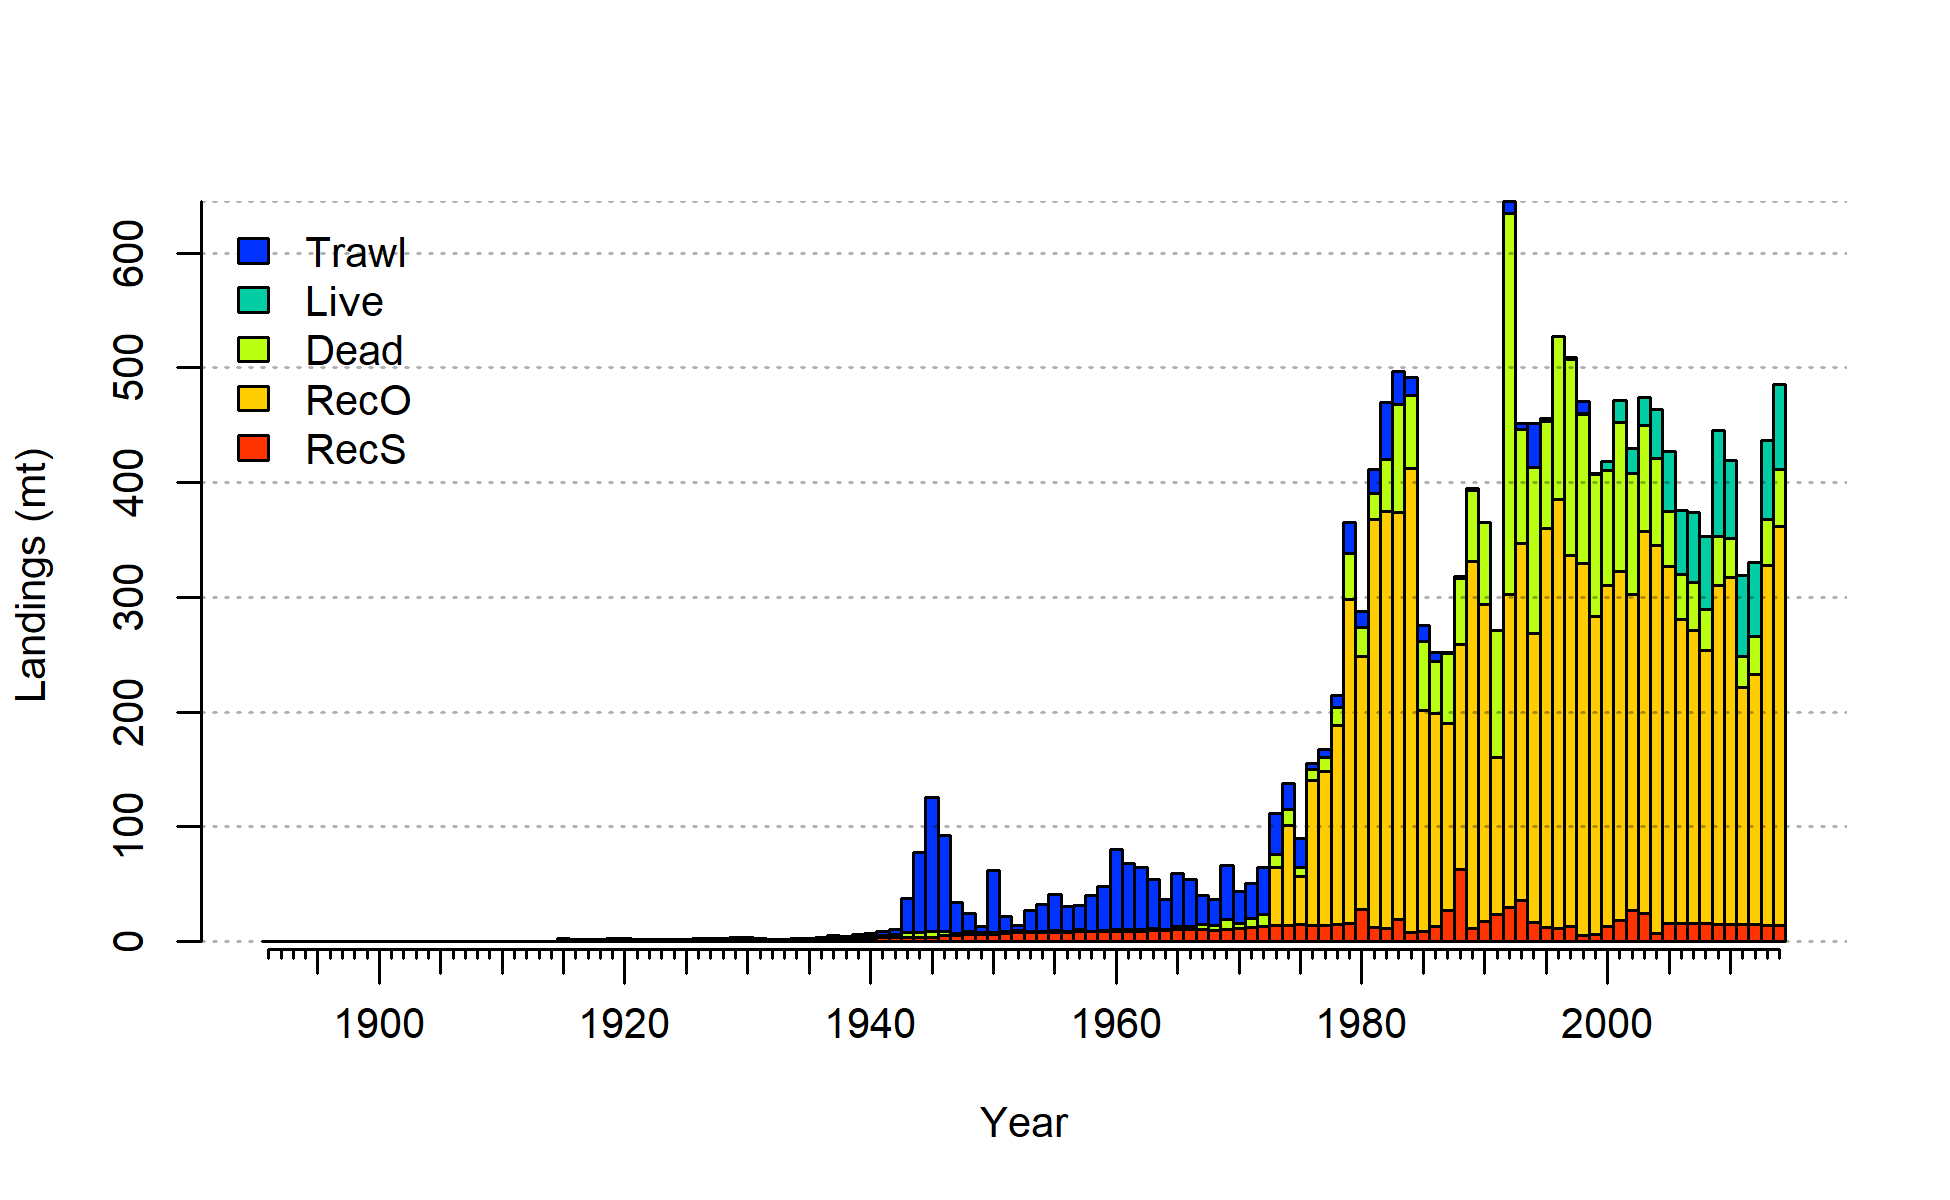
\includegraphics[width=1\textwidth,height=1\textheight]{C:/Users/Jason.Cope/Documents/Github/Sebastes_melanops_WA/Document/models/Reference model/plots/catch2 landings stacked.png}
\caption{Landings by fleet used in the reference model where catches in metric tons by fleet are stacked.\label{fig:es-catch}}
\end{figure}

\clearpage

\hypertarget{data-and-assessment}{%
\subsection*{Data and assessment}\label{data-and-assessment}}
\addcontentsline{toc}{subsection}{Data and assessment}

The last stock assessments for black rockfish were conducted in 2007 for areas north and south of Cape Falcon (45\textdegree46' North latitude). The current assessments assume three areas instead of two, delineated by the state lines as was agreed upon at a pre-assessment and data workshop in March 2015. The prior assessments used Stock Synthesis 2, while the current assessments use Stock Synthesis

\begin{verbatim}
[1] "3.30.20.00"
\end{verbatim}

. The Washington base assessment includes a dockside and tag-based CPUE series, but does not include the abundance estimate time series from that same tagging study which was included in the last assessment due to too many violations in the assumptions of abundance estimation. The same two commercial and single recreational fleets are used as in the last assessment for Washington. The Oregon assessment has three commercial fleets and two recreational fleets, while using five surveys and an additional research study for biological compositions. California also has three commercial fleets and 1 recreational fleet with three surveys of abundance, all based on recreational fisheries. All area models include age data as conditional age at lengths. Length compositions are also included in all models.

The stock assessment for Black Rockfish off Oregon was developed using the length- and age-structured model Stock Synthesis (version 3.30.16). No previous stock assessment for Black Rockfish off Oregon has been conducted. Model structure included two fleets (commercial and recreational) and one fishery-based index of abundance. Life history parameters were sex-specific (i.e., a two-sex model) with natural mortality and growth parameters estimated, along with recruitment. The model covers the years 1892 to 2014, with a 12 year forecast beginning in 2015.

This assessment integrates data and information from multiple sources into one modeling framework. Specifically, the assessment uses landings data, length and conditional age-at-length composition data (using ageing error matrices to incorporate ageing imprecision) for each fishery, and one index of abundance based on the recreational fishery; fixed parameterizations of weight-at-length, maturity-at-length, and fecundity-at-length, the Beverton-Holt stock-recruitment steepness value and recruitment variability. Estimated values include initial population scale (\(lnR_0\)), natural mortality and growth for each sex, asymptotic selectivity and recruitment deviations. The base model was tuned to account for the weighting of the length and age data and index variances (which was estimated), as well as the specification of recruitment variance and recruitment bias adjustments. Derived quantities include the time series of spawning biomass, age and size structure, and current and projected future stock status.

Within model uncertainty is explicitly included in this assessment by parameter estimation uncertainty, while among model uncertainty is explored through sensitivity analyses addressing alternative input assumptions such as data treatment and weighting, and model specification sensitivity to the treatment of life history parameters, selectivity, and recruitment. A reference model was selected that best fit the observed data while concomitantly balancing the desire to capture the central tendency across those sources of uncertainty, ensure model realism and tractability, and promote robustness to potential model misspecification.

\hypertarget{stock-biomass-and-dynamics}{%
\subsection*{Stock biomass and dynamics}\label{stock-biomass-and-dynamics}}
\addcontentsline{toc}{subsection}{Stock biomass and dynamics}

Spawning stock outputs are all at or above limit reference points (Table ES-2. Only California shows declines significantly below this reference point at any point in the time series. California and Washington stocks show a declining population through most of the 20th Century, with stronger declines in the 1980s, and recoveries beginning in the mid-1990s. Oregon stocks follow this pattern, but with a decline in the most recent period. California (33\%) is below the target biomass reference point with an increasing biomass trend (Figures ES-4 and ES-5). The Oregon stock dropped after the quick ramp up of catches in the late 1970s and continued a steady decline until around year 2000, settling in at a stock status around 60\% of initial conditions. The Washington stock, currently 43\%, dropped below the target biomass by in the early 1980s, then risen above since the late 1990s and has fluctuated above that point through 2014 (Figures ES-8 and ES-9).

Spawning output (in millions of eggs; meggs) instead of spawning biomass is used to report the mature population scale because fecundity is nonlinearly related to body female weight. The estimated spawning output at the beginning of 2021 was 830 meggs (\textasciitilde95 percent asymptotic intervals: 807 to 852 meggs, Table \ref{tab:ssbES} and Figure \ref{fig:es-ssb}), which when compared to unfished spawning output (1,376) meggs gives a relative stock status level of 60 percent (\textasciitilde95 percent asymptotic intervals: 60 to 61 percent, Figure \ref{fig:es-depl}). Overall, spawning output declined with the onset of increasing commercial removals in the 1960s and continued to decline with the increase in recreational catches through the 1990s, even dropping below the target relative stock size. The largest of the estimated recruitment pulses since the mid 1990s (that are supported by each of the data sets) caused a sharp increase in spawning output through the mid 2010s, followed by another decline. The minimum relative stock size of 59 percent of unfished levels is estimated to have occurred in 2006. Currently the stock is estimated well above the management target of \(SB_{40\%}\) in 2021 and is estimated to have remained above the target since 2000 (Table \ref{tab:ssbES} and Figure \ref{fig:es-depl}).

\begingroup\fontsize{10}{12}\selectfont
\begingroup\fontsize{10}{12}\selectfont

\begin{longtable}[t]{r>{\centering\arraybackslash}p{1.57cm}>{\centering\arraybackslash}p{1.57cm}>{\centering\arraybackslash}p{1.57cm}>{\centering\arraybackslash}p{1.57cm}>{\centering\arraybackslash}p{1.57cm}>{\centering\arraybackslash}p{1.57cm}}
\caption{\label{tab:ssbES}Estimated recent trend in spawning output and the fraction unfished and the 95 percent intervals.}\\
\toprule
Year & Spawning Output & Lower Interval & Upper Interval & Fraction Unfished & Lower Interval & Upper Interval\\
\midrule
\endfirsthead
\caption[]{Estimated recent trend in spawning output and the fraction unfished and the 95 percent intervals. \textit{(continued)}}\\
\toprule
Year & Spawning Output & Lower Interval & Upper Interval & Fraction Unfished & Lower Interval & Upper Interval\\
\midrule
\endhead

\endfoot
\bottomrule
\endlastfoot
2013 & 239.61 & 189.29 & 289.93 & 0.25 & 0.21 & 0.29\\
2014 & 249.53 & 192.38 & 306.68 & 0.26 & 0.22 & 0.31\\
2015 & 261.05 & 195.22 & 326.88 & 0.27 & 0.22 & 0.33\\
2016 & 274.76 & 198.39 & 351.13 & 0.29 & 0.23 & 0.35\\
2017 & 289.73 & 200.98 & 378.47 & 0.31 & 0.23 & 0.38\\
2018 & 319.12 & 216.03 & 422.21 & 0.34 & 0.25 & 0.42\\
2019 & 346.49 & 227.88 & 465.10 & 0.36 & 0.27 & 0.46\\
2020 & 372.63 & 238.20 & 507.06 & 0.39 & 0.28 & 0.51\\
2021 & 406.97 & 257.39 & 556.55 & 0.43 & 0.30 & 0.56\\
2022 & 425.64 & 263.13 & 588.16 & 0.45 & 0.31 & 0.59\\
2023 & 439.55 & 266.93 & 612.16 & 0.46 & 0.31 & 0.61\\*
\end{longtable}
\endgroup{}
\endgroup{}


\begin{figure}
\centering
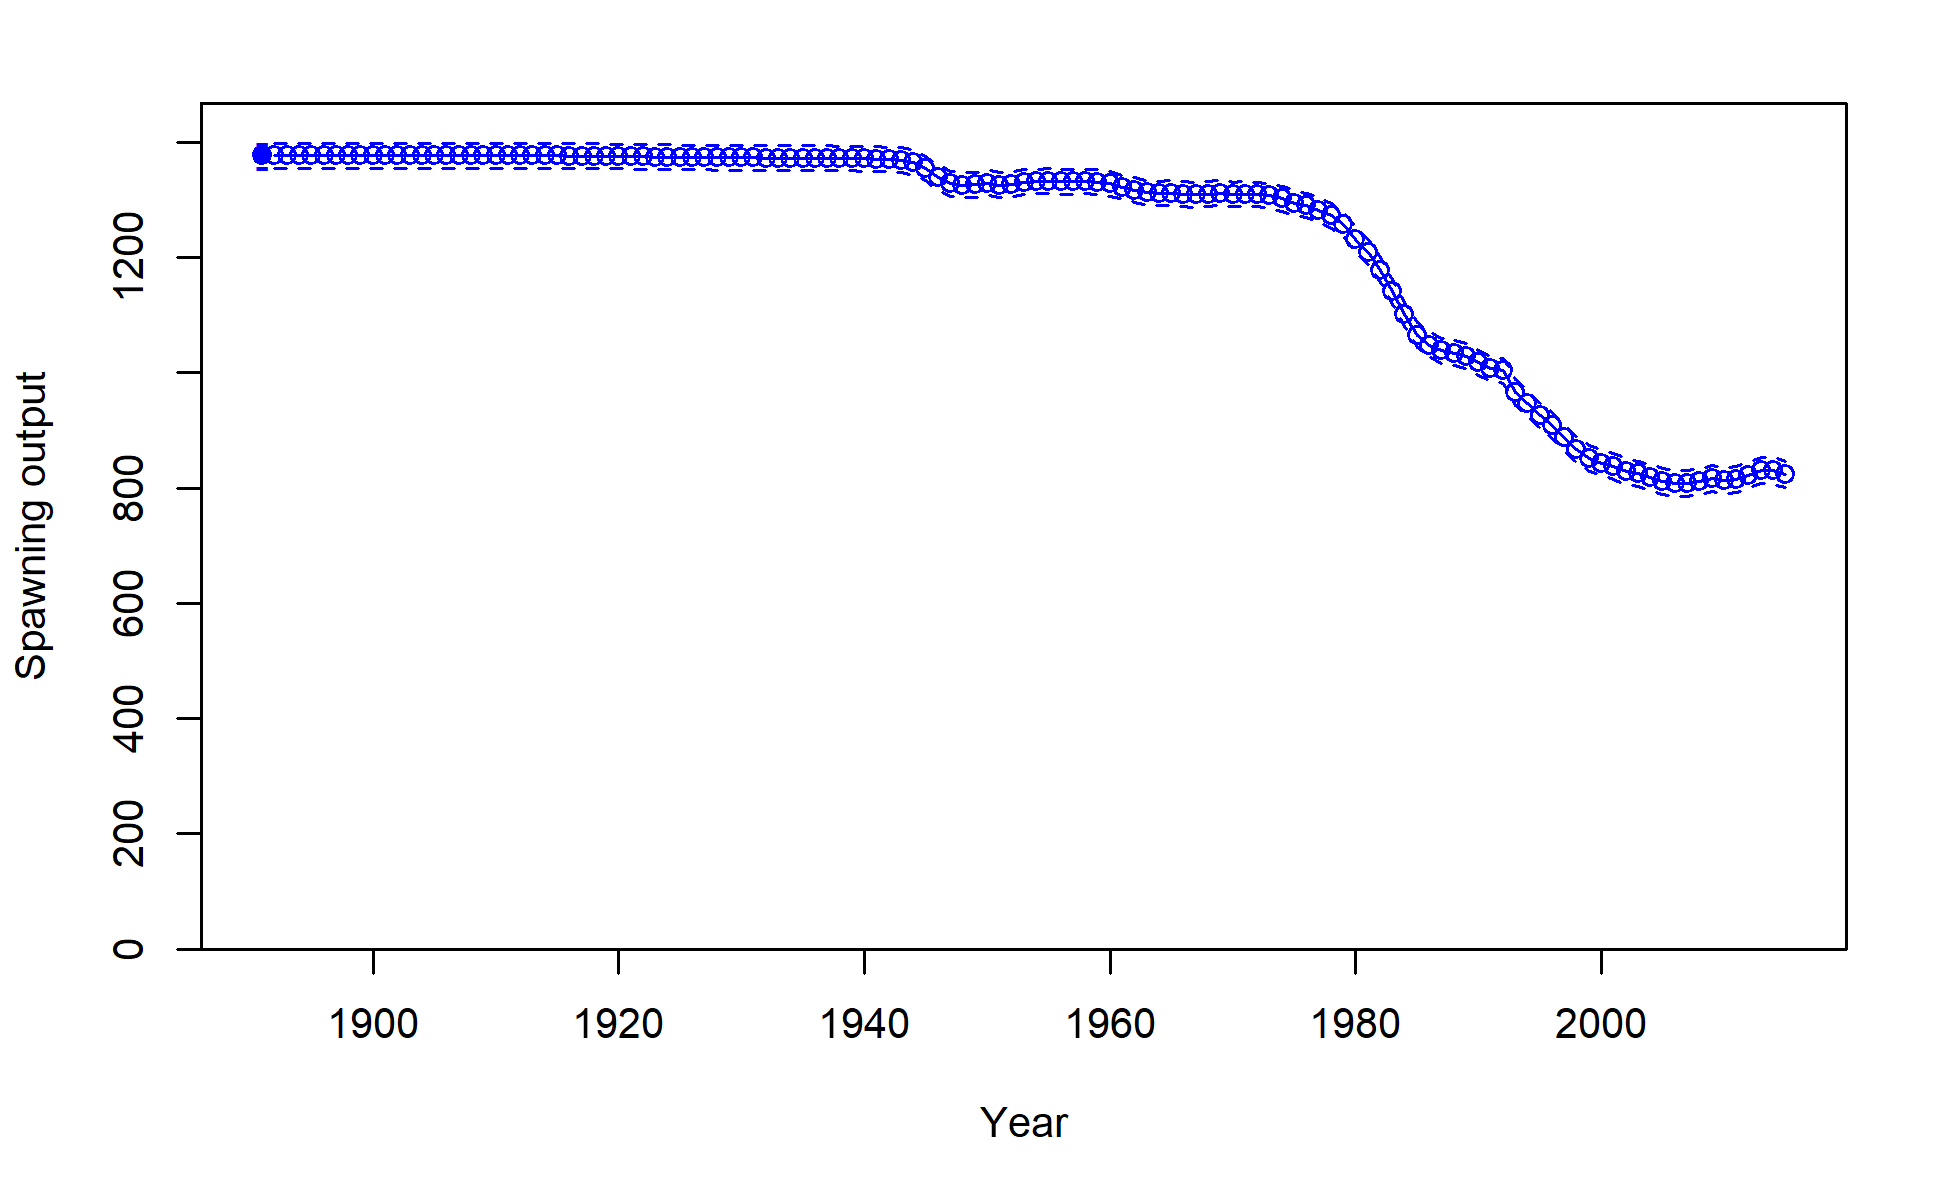
\includegraphics[width=1\textwidth,height=1\textheight]{C:/Users/Jason.Cope/Documents/Github/Sebastes_melanops_WA/Document/models/Reference model/plots/ts7_Spawning_output_with_95_asymptotic_intervals_intervals.png}
\caption{Estimated time series of spawning output (circles and line: median; light broken lines: 95 percent intervals) for the base model.\label{fig:es-ssb}}
\end{figure}

\begin{figure}
\centering
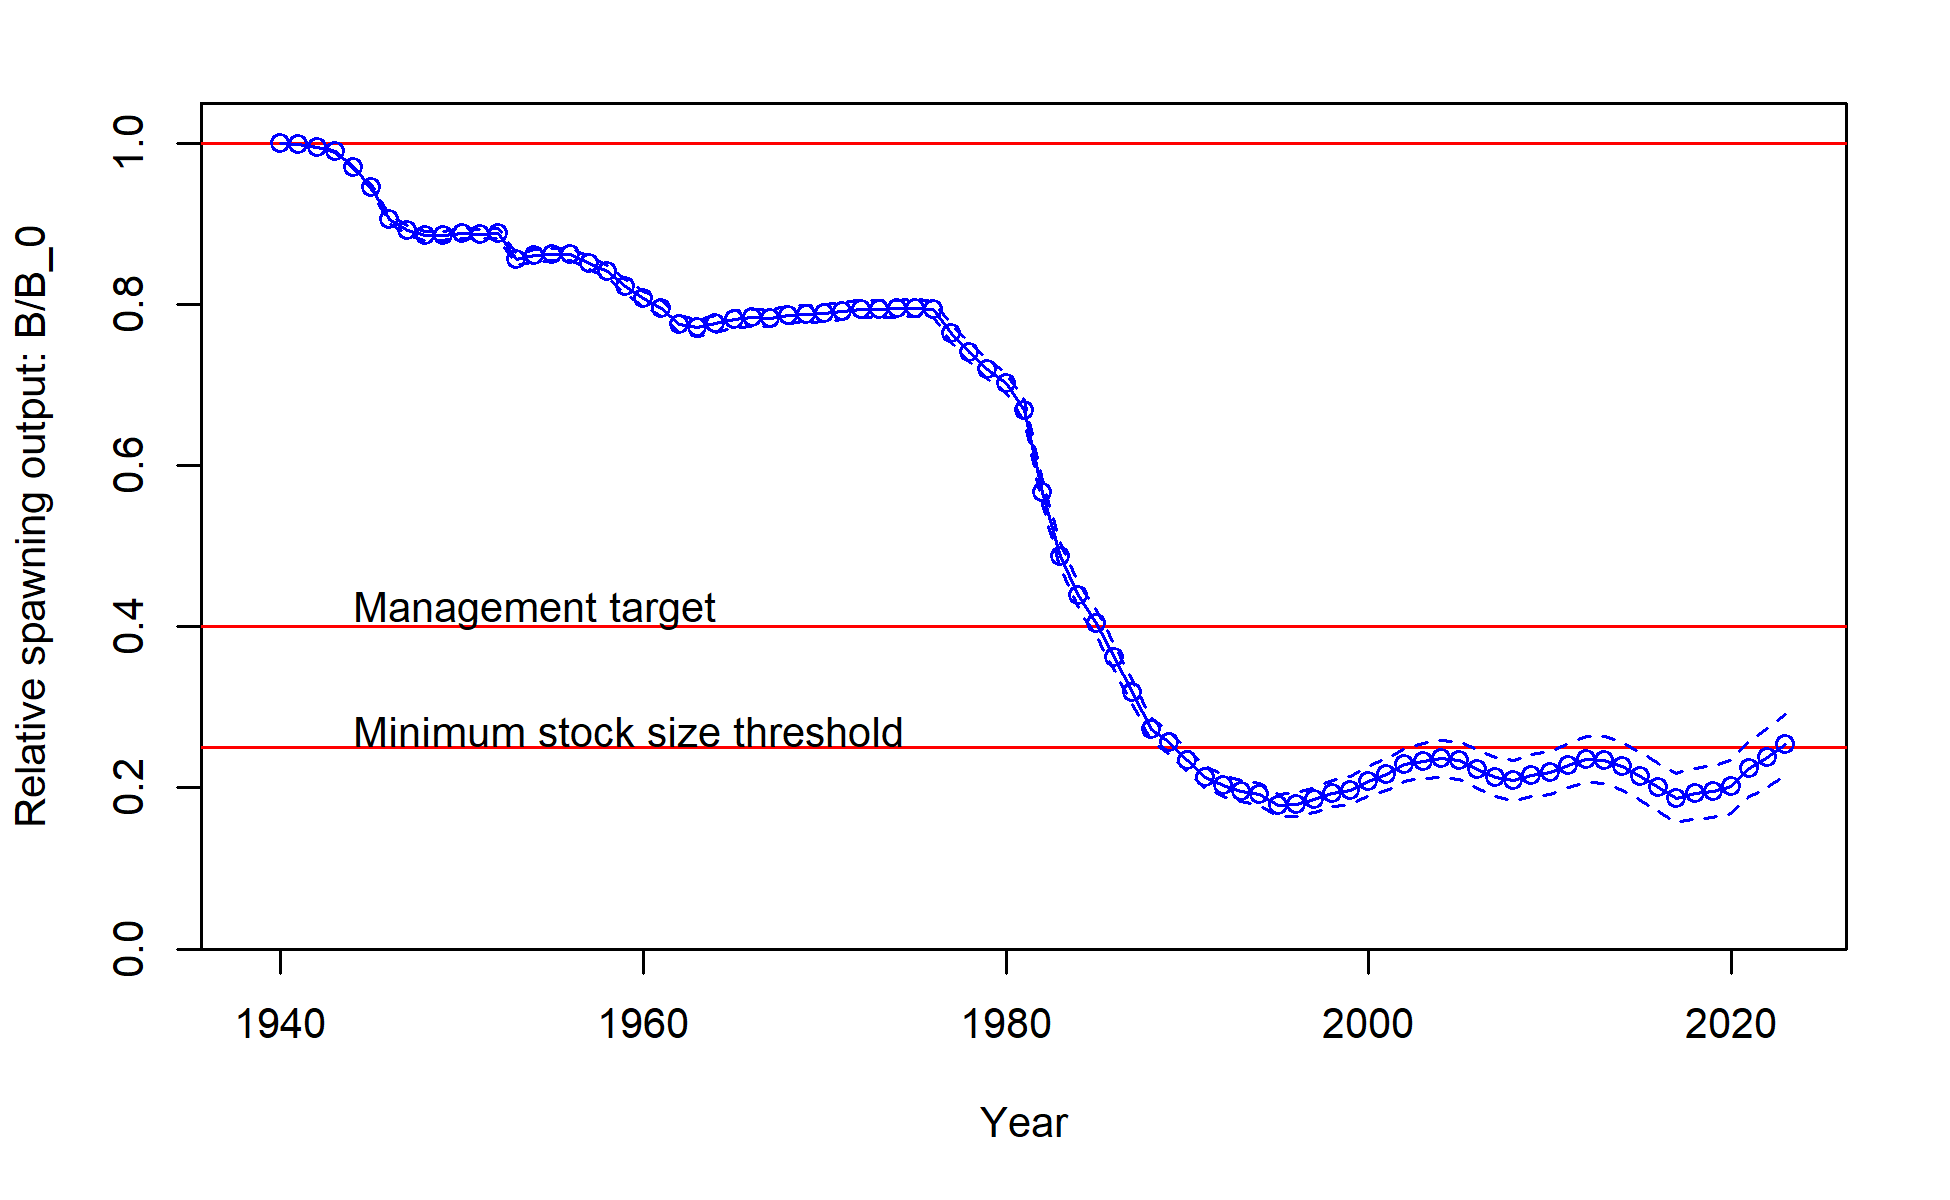
\includegraphics[width=1\textwidth,height=1\textheight]{C:/Users/Jason.Cope/Documents/Github/Sebastes_melanops_WA/Document/models/Reference model/plots/ts9_Relative_spawning_output_intervals.png}
\caption{Estimated time series of fraction of unfished spawning output (circles and line: median; light broken lines: 95 percent intervals) for the base model.\label{fig:es-depl}}
\end{figure}

\clearpage

\hypertarget{recruitment}{%
\subsection*{Recruitment}\label{recruitment}}
\addcontentsline{toc}{subsection}{Recruitment}

The California model shows a few extraordinarily high recruitment events that are supported by the length composition data, index data and on-the-water reports (Table ES-3; Figure ES-10). Oregon recruitment is highly uncertain (Table ES-3; Figure ES11). Washington recruitment is dynamic, but also shows the most informed recruitment time series, which is consistent with the extent of length and age compositions available to that assessment (Table ES-3; Figure ES12). Both California and Washington support elevated recruitment in the late 2000s.

Informative recruitment begins in the 1960s and peaks in the 1990s (Table \ref{tab:recrES} and Figure \ref{fig:es-recruits}). Data were most informative from the the 1990s to the mid-2010s. Peaks years of recruitments are found in years 1993, 1994, 1998, 2005 and 2015 (Figure \ref{fig:es-rec-devs}). Overall, the Black Rockfish stock has not been reduced to levels that would provide considerable information on how recruitment compensation changes across spawning biomass levels (i.e., inform the steepness parameter). Thus, all recruitment is based on a fixed assumption about steepness (\(h\) = 0.72) and recruitment variability (\(\sigma_R\) = 0.6).

\begingroup\fontsize{10}{12}\selectfont
\begingroup\fontsize{10}{12}\selectfont

\begin{longtable}[t]{r>{\centering\arraybackslash}p{1.57cm}>{\centering\arraybackslash}p{1.57cm}>{\centering\arraybackslash}p{1.57cm}>{\centering\arraybackslash}p{1.57cm}>{\centering\arraybackslash}p{1.57cm}>{\centering\arraybackslash}p{1.57cm}}
\caption{\label{tab:recrES}Estimated recent trend in recruitment and recruitment deviations and the 95 percent intervals.}\\
\toprule
Year & Recruitment & Lower Interval & Upper Interval & Recruitment Deviations & Lower Interval & Upper Interval\\
\midrule
\endfirsthead
\caption[]{Estimated recent trend in recruitment and recruitment deviations and the 95 percent intervals. \textit{(continued)}}\\
\toprule
Year & Recruitment & Lower Interval & Upper Interval & Recruitment Deviations & Lower Interval & Upper Interval\\
\midrule
\endhead

\endfoot
\bottomrule
\endlastfoot
2013 & 1972.96 & 1304.38 & 2984.22 & 0.42 & 0.08 & 0.77\\
2014 & 1524.90 & 970.90 & 2395.02 & 0.15 & -0.23 & 0.54\\
2015 & 1117.78 & 678.00 & 1842.81 & -0.17 & -0.61 & 0.27\\
2016 & 1222.12 & 732.14 & 2040.03 & -0.12 & -0.57 & 0.34\\
2017 & 745.60 & 383.36 & 1450.13 & -0.65 & -1.28 & -0.02\\
2018 & 1640.14 & 1429.19 & 1882.23 & 0.00 & 0.00 & 0.00\\
2019 & 1671.35 & 1454.43 & 1920.62 & 0.00 & 0.00 & 0.00\\
2020 & 1697.60 & 1475.50 & 1953.13 & 0.00 & 0.00 & 0.00\\
2021 & 1728.44 & 1505.90 & 1983.87 & 0.00 & 0.00 & 0.00\\
2022 & 1742.76 & 1516.49 & 2002.79 & 0.00 & 0.00 & 0.00\\
2023 & 1752.52 & 1523.38 & 2016.13 & 0.00 & 0.00 & 0.00\\*
\end{longtable}
\endgroup{}
\endgroup{}


\begin{figure}
\centering
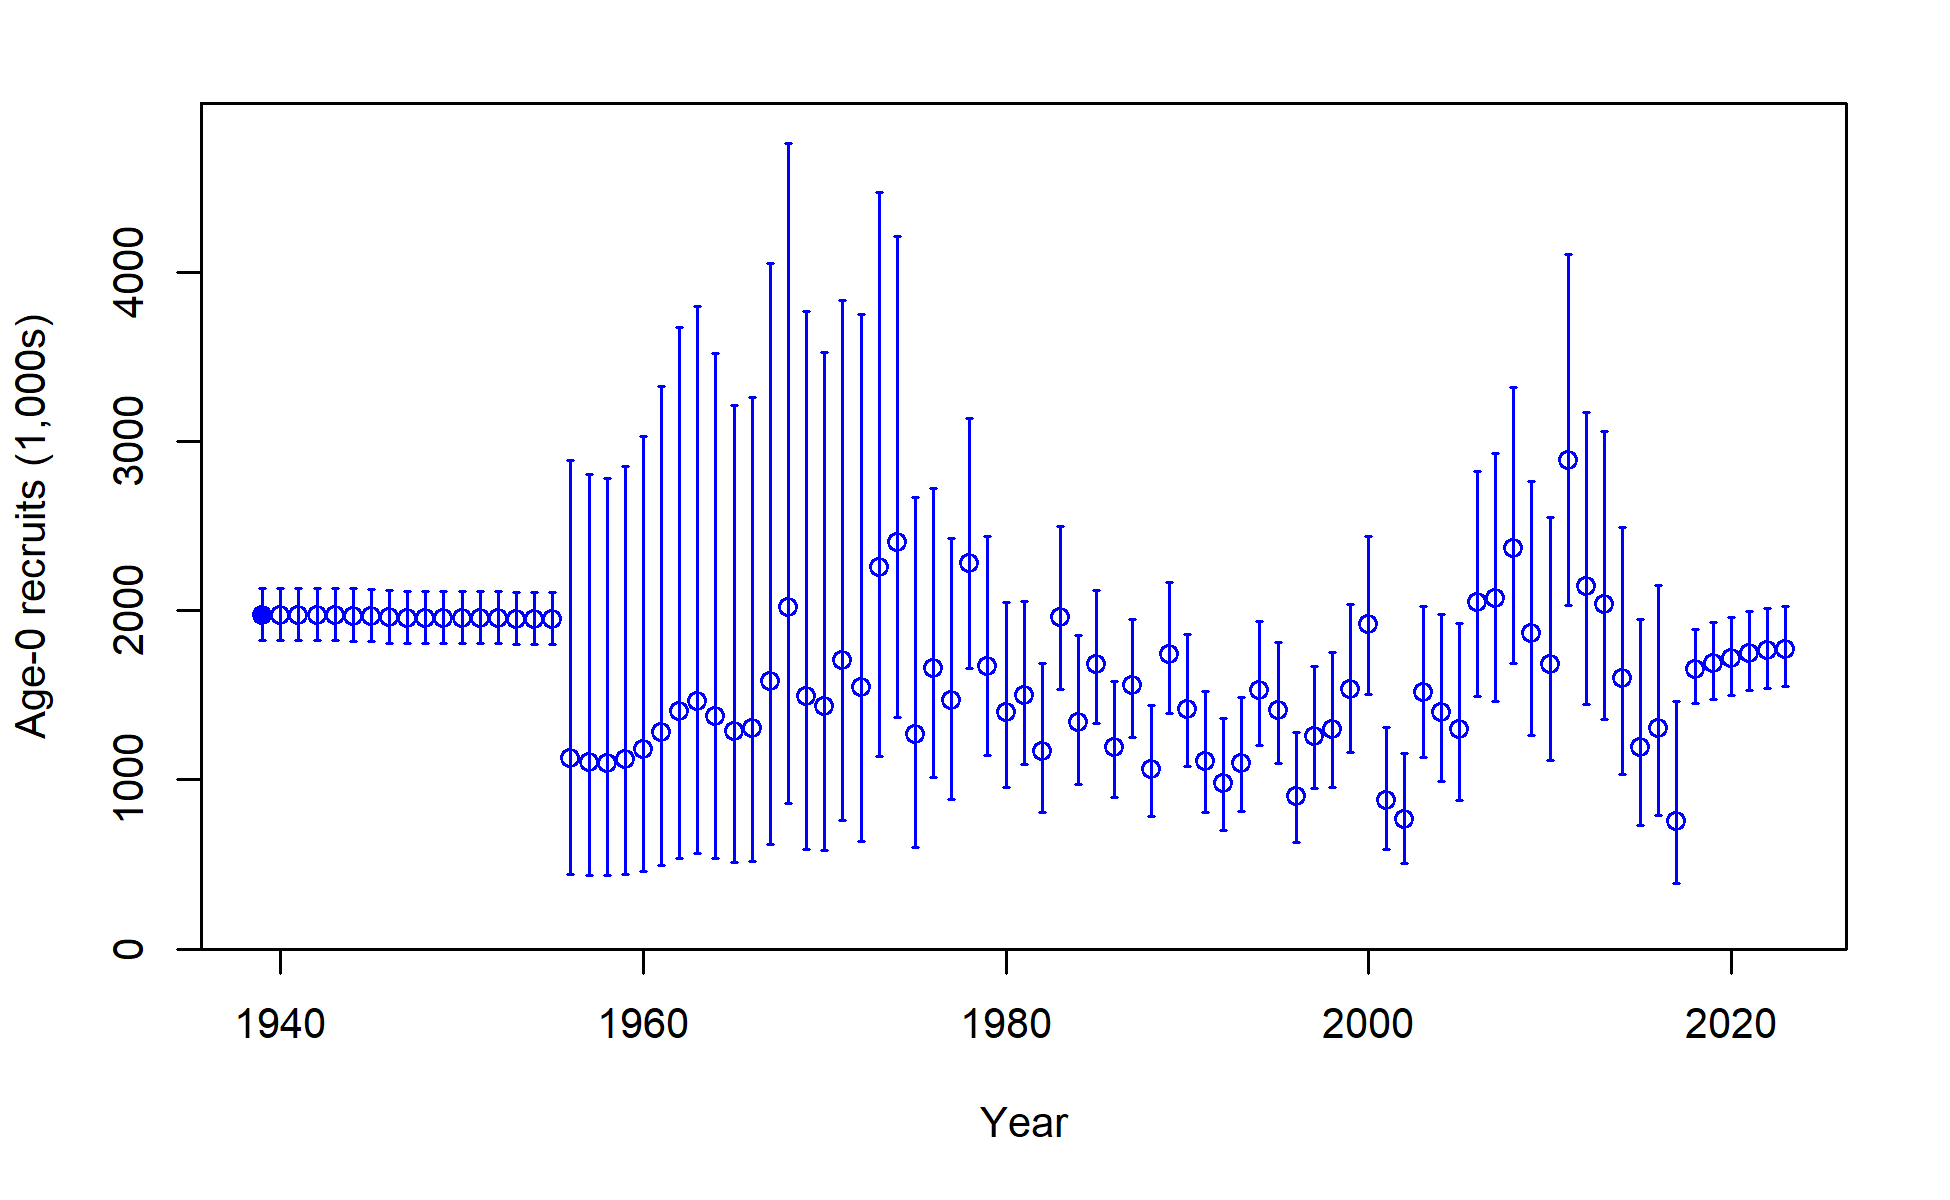
\includegraphics[width=1\textwidth,height=1\textheight]{C:/Users/Jason.Cope/Documents/Github/Sebastes_melanops_WA/Document/models/Reference model/plots/ts11_Age-0_recruits_(1000s)_with_95_asymptotic_intervals.png}
\caption{Estimated time series of age-0 recruits (1000s) for the base model with 95 percent intervals.\label{fig:es-recruits}}
\end{figure}

\#\texttt{\{r,\ results\ =\ \textquotesingle{}asis\textquotesingle{}\}\ \#add\_figure(\ \#filein\ =\ file.path(mod\_loc,\ "plots",\ "recdevs2\_withbars.png"),\ \ \#caption\ =\ "Estimated\ time\ series\ of\ recruitment\ deviations",\ \#label\ =\ \textquotesingle{}es-rec-devs\textquotesingle{})\ \#}

\hypertarget{exploitation-status}{%
\subsection*{Exploitation status}\label{exploitation-status}}
\addcontentsline{toc}{subsection}{Exploitation status}

California and Washington models indicate that current fishing practices are near or above the SPR rate fishing intensity target, while the Oregon model is quite a bit above the target (table ES-4, compare to SPR=0.5; Figure ES-13 to Figure ES-18), though the steepness value (0.773) indicates a much lower value of SPR for sustainable removals. Fishing rates have been above the target in California in nearly all years since the 1980s, but have dropped considerably in recent years. Oregon fishing rates have been consistently high in recent years. Washington shows a dramatic decline in fishing intensity since the late 1990s and has fluctuated mostly below the target since.

Trends in fishing intensity (1 - SPR) largely mirrored that of landings until the 1990s when recruitment pulses overcame the catches to lower overall fishing intensity (Figure \ref{fig:es-1-spr}). The maximum fishing intensity was 0.49 in 1992, above the target SPR-based harvest rate of 0.50 (1 - \(\text{SPR}_{50\%}\)). Current levels of 0.39 for 2020 are near the fishing limit. Fishing intensity over the past decade has ranged between 0.31 and 0.42 and the exploitation rate has been high (0.04 - 0.06, Table \ref{tab:exploitES}). Current estimates indicate that Black Rockfish spawning output is much greater than than the target biomass level (\(\text{SB}_{40\%}\)), though fishing intensity remains near target \(F_{MSY}\) proxy harvest rate.

\begingroup\fontsize{10}{12}\selectfont
\begingroup\fontsize{10}{12}\selectfont

\begin{longtable}[t]{r>{\centering\arraybackslash}p{1.57cm}>{\centering\arraybackslash}p{1.57cm}>{\centering\arraybackslash}p{1.57cm}>{\centering\arraybackslash}p{1.57cm}>{\centering\arraybackslash}p{1.57cm}>{\centering\arraybackslash}p{1.57cm}}
\caption{\label{tab:exploitES}Estimated recent trend in the 1-SPR where SPR is the spawning potential ratio the exploitation rate, and the  95 percent intervals.}\\
\toprule
Year & 1-SPR & Lower Interval & Upper Interval & Exploitation Rate & Lower Interval & Upper Interval\\
\midrule
\endfirsthead
\caption[]{Estimated recent trend in the 1-SPR where SPR is the spawning potential ratio the exploitation rate, and the  95 percent intervals. \textit{(continued)}}\\
\toprule
Year & 1-SPR & Lower Interval & Upper Interval & Exploitation Rate & Lower Interval & Upper Interval\\
\midrule
\endhead

\endfoot
\bottomrule
\endlastfoot
2013 & 0.65 & 0.60 & 0.71 & 0.06 & 0.05 & 0.08\\
2014 & 0.67 & 0.60 & 0.73 & 0.07 & 0.05 & 0.08\\
2015 & 0.66 & 0.59 & 0.73 & 0.07 & 0.05 & 0.09\\
2016 & 0.65 & 0.57 & 0.73 & 0.07 & 0.05 & 0.09\\
2017 & 0.52 & 0.43 & 0.61 & 0.05 & 0.03 & 0.06\\
2018 & 0.53 & 0.43 & 0.62 & 0.05 & 0.03 & 0.07\\
2019 & 0.50 & 0.40 & 0.59 & 0.05 & 0.03 & 0.07\\
2020 & 0.32 & 0.23 & 0.40 & 0.03 & 0.02 & 0.03\\
2021 & 0.41 & 0.31 & 0.51 & 0.04 & 0.03 & 0.05\\
2022 & 0.37 & 0.27 & 0.46 & 0.03 & 0.02 & 0.04\\*
\end{longtable}
\endgroup{}
\endgroup{}


\begin{figure}
\centering
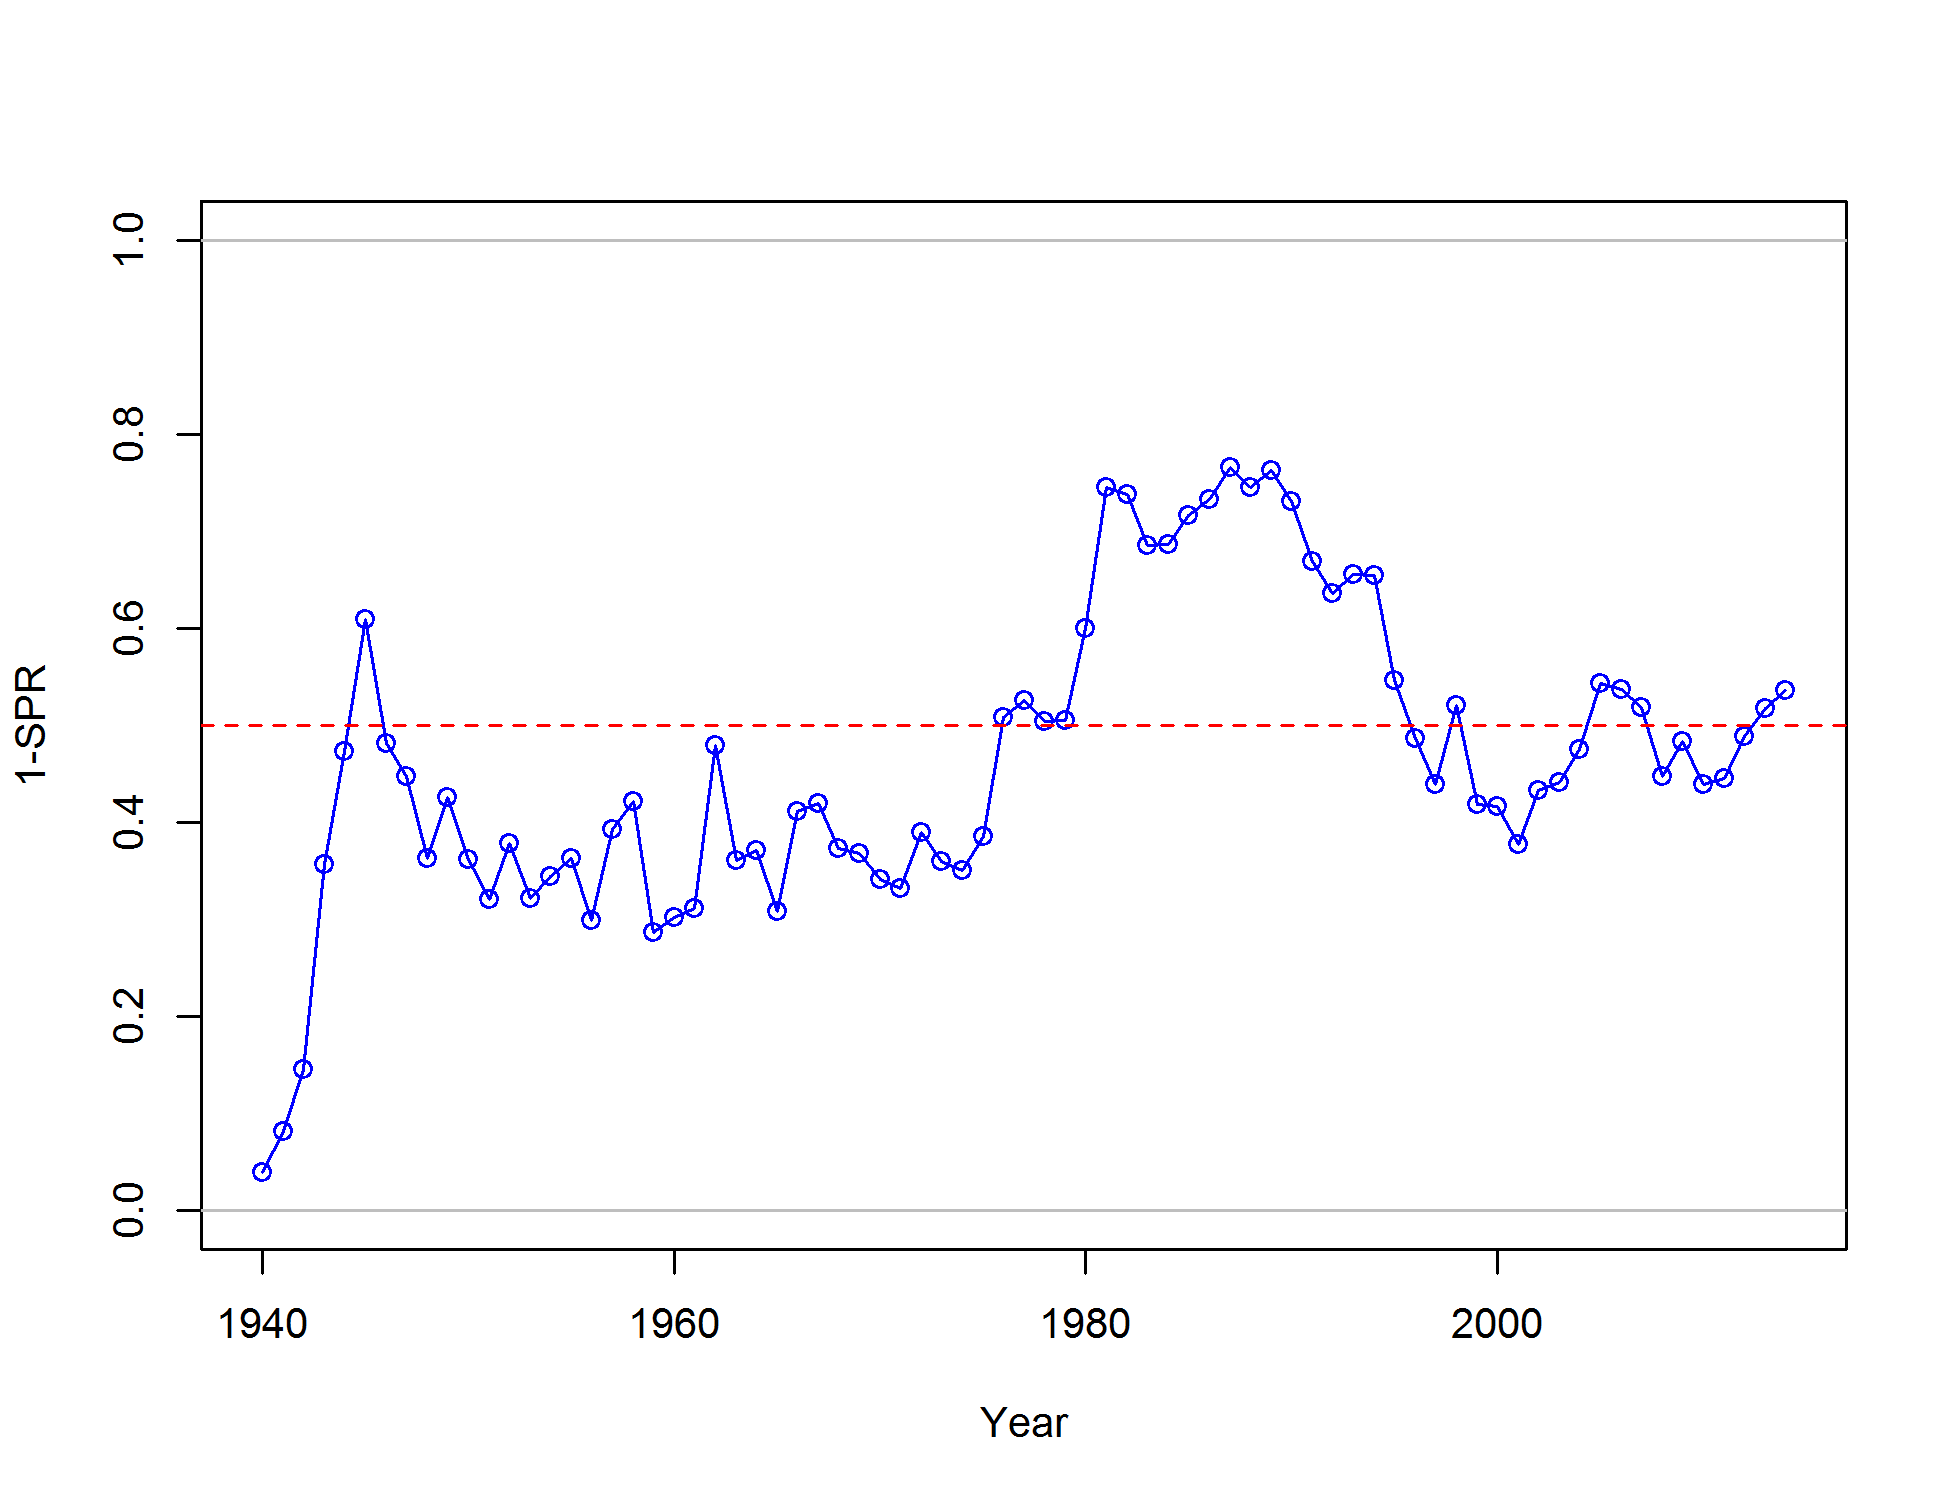
\includegraphics[width=1\textwidth,height=1\textheight]{C:/Users/Jason.Cope/Documents/Github/Sebastes_melanops_WA/Document/models/Reference model/plots/SPR2_minusSPRseries.png}
\caption{Estimated 1 - relative spawning ratio (SPR) by year for the base model. The management target is plotted as a red horizontal line and values above this reflect harvest in excess of the proxy harvest rate.\label{fig:es-1-spr}}
\end{figure}

\clearpage

\hypertarget{ecosystem-considerations}{%
\subsection*{Ecosystem considerations}\label{ecosystem-considerations}}
\addcontentsline{toc}{subsection}{Ecosystem considerations}

This stock assessment does not explicitly incorporate trophic interactions, habitat factors or environmental factors into the assessment model. More predation, diet and habitat work, and mechanistic linkages to environmental conditions would be needed to incorporate these elements into the stock assessment. While no mechanisms have been put forth for these time-varying changes in growth, an environmental component is possible. Limited data in Oregon and California also suggest the possibility that growth has changed over time.

\hypertarget{reference-points}{%
\subsection*{Reference points}\label{reference-points}}
\addcontentsline{toc}{subsection}{Reference points}

Reference points were based on the rockfish FMSY proxy (SPR50\%), target relative biomass (40\%) and model-estimated selectivity for each fleet. California is below the target biomass reference point, but above the limit reference biomass (25\%). Oregon is well above the target biomass. Washington relative biomass is above the target biomass. California and Washington yield values are lower than the previous assessment for similar reference points due to lower overall natural mortality values (Table ES-5). The proxy MSY values of management quantities are the most conservative compared to the estimated MSY and MSY relative to 40\% biomass for both California and Washington (Table ES-5). The equilibrium estimates of yield relative to biomass are provided in Figure ES-19 to Figure ES-21.

The 2021 spawning biomass relative to unfished equilibrium spawning biomass is well above the management target of 40 percent of unfished spawning biomass. The relative biomass and the ratio of the estimated SPR to the management target (\(\text{SPR}_{50\%}\)) across all model years are shown in Figure \ref{fig:es-phase} where warmer colors (red) represent early years and colder colors (blue) represent recent years. There have been periods where the stock status has decreased below the target and fishing intensity has been higher than the target fishing intensity based on \(\text{SPR}_{50\%}\). Figure \ref{fig:es-yield} shows the equilibrium curve based on a steepness value fixed at 0.77 with vertical dashed lines to indicate the estimate of fraction unfished at the start of 2015 (current) and the estimated management targets calculated based on the relative target biomass (B target), the SPR target, and the maximum sustainable yield (MSY).

Reference points were calculated using the estimated selectivities and catch distributions among fleets in the most recent year of the model, 2014 (Table \ref{tab:e_ReferencePoints_ES}). Sustainable total yield, removals, using an \(\text{SPR}_{50\%}\) is 514 mt. The spawning output equivalent to 40 percent of the unfished spawning output (\(\text{SO}_{40\%}\)) calculated using the SPR target (\(\text{SPR}_{50\%}\)) was 633.7 meggs. Recent removals have been close to the point estimate of potential long-term yields calculated using an \(\text{SPR}_{50\%}\) reference point and the population size has been relatively decreasing toward the target over the past few years.

\begin{figure}
\centering
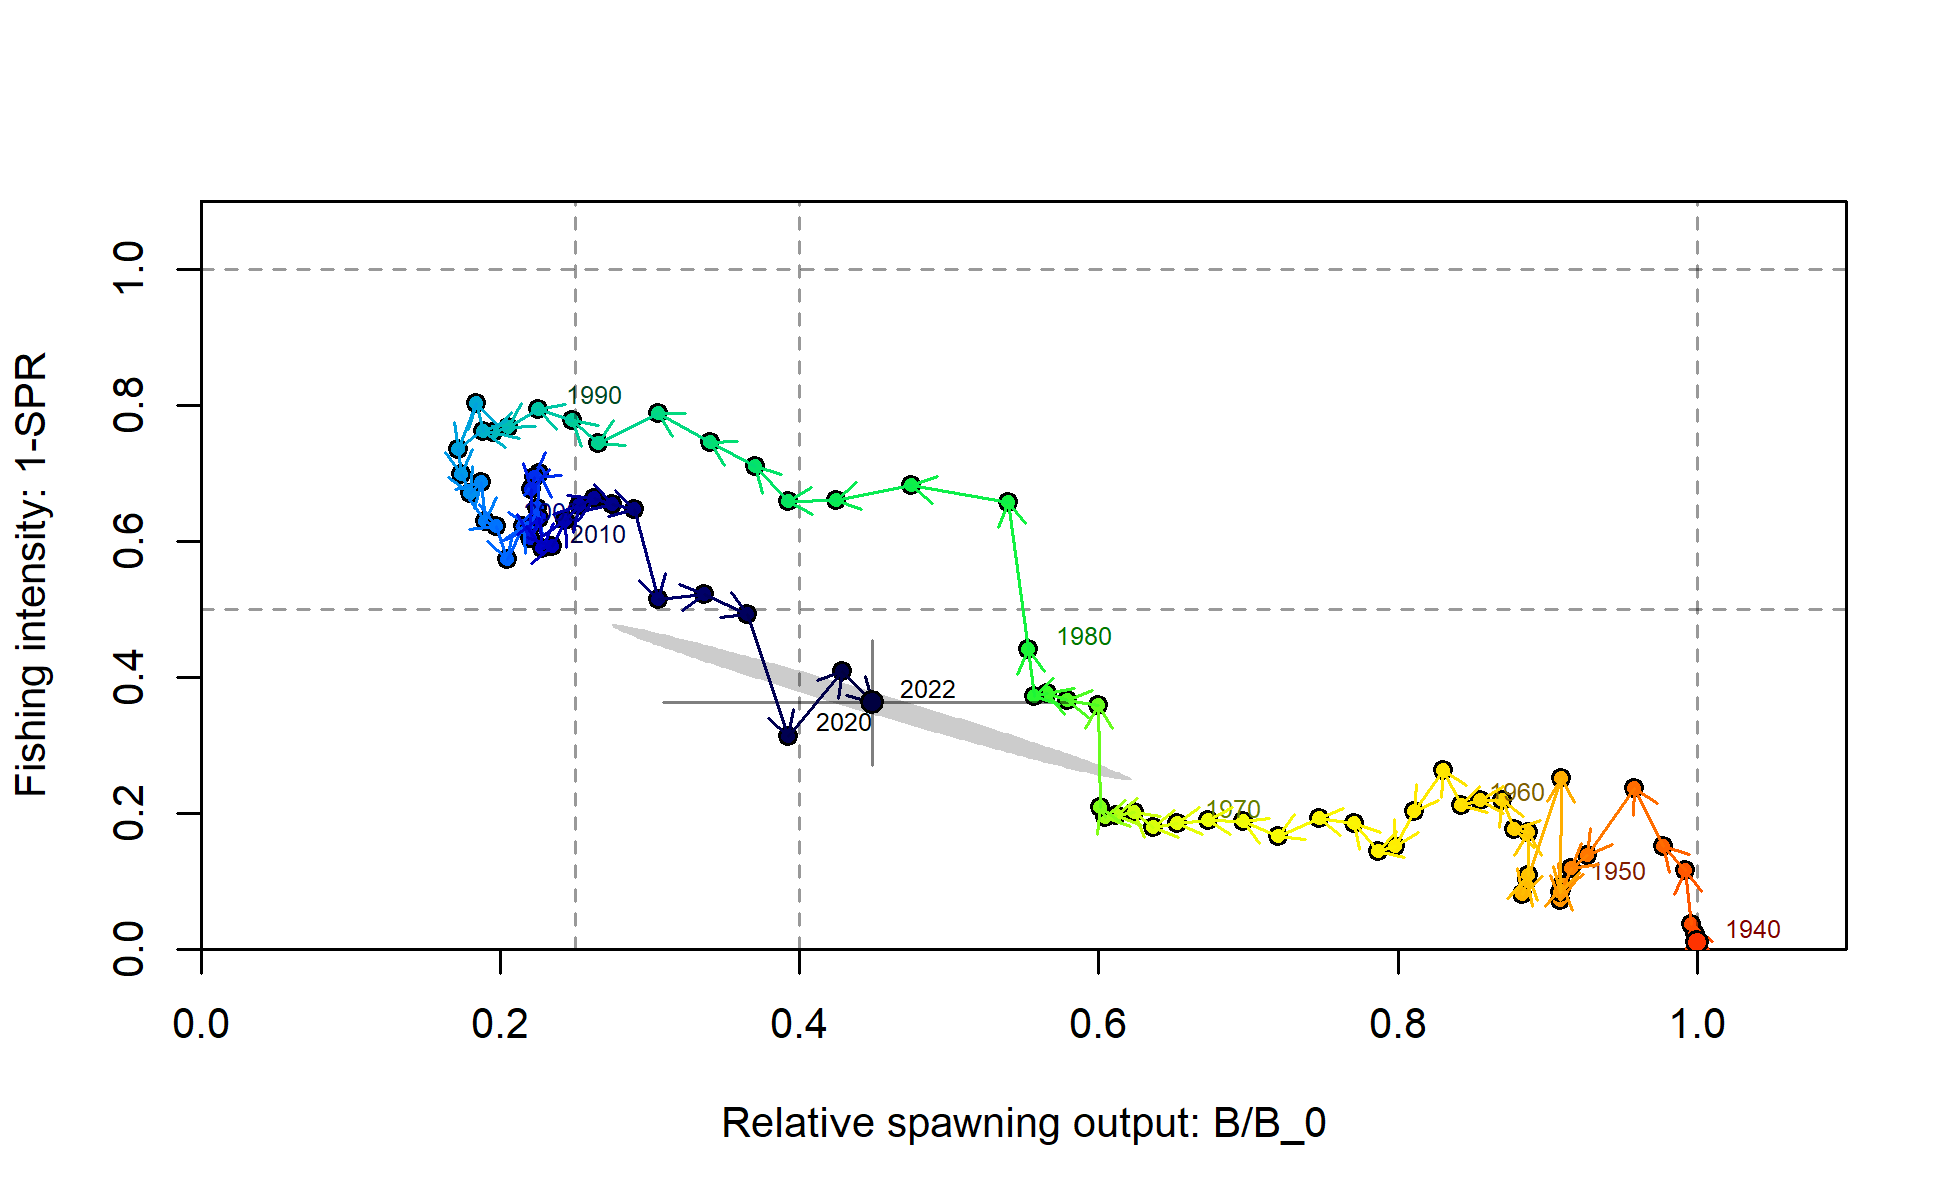
\includegraphics[width=1\textwidth,height=1\textheight]{C:/Users/Jason.Cope/Documents/Github/Sebastes_melanops_WA/Document/models/Reference model/plots/SPR4_phase.png}
\caption{Phase plot of estimated 1-SPR versus fraction unfished for the base model.\label{fig:es-phase}}
\end{figure}

\begin{figure}
\centering
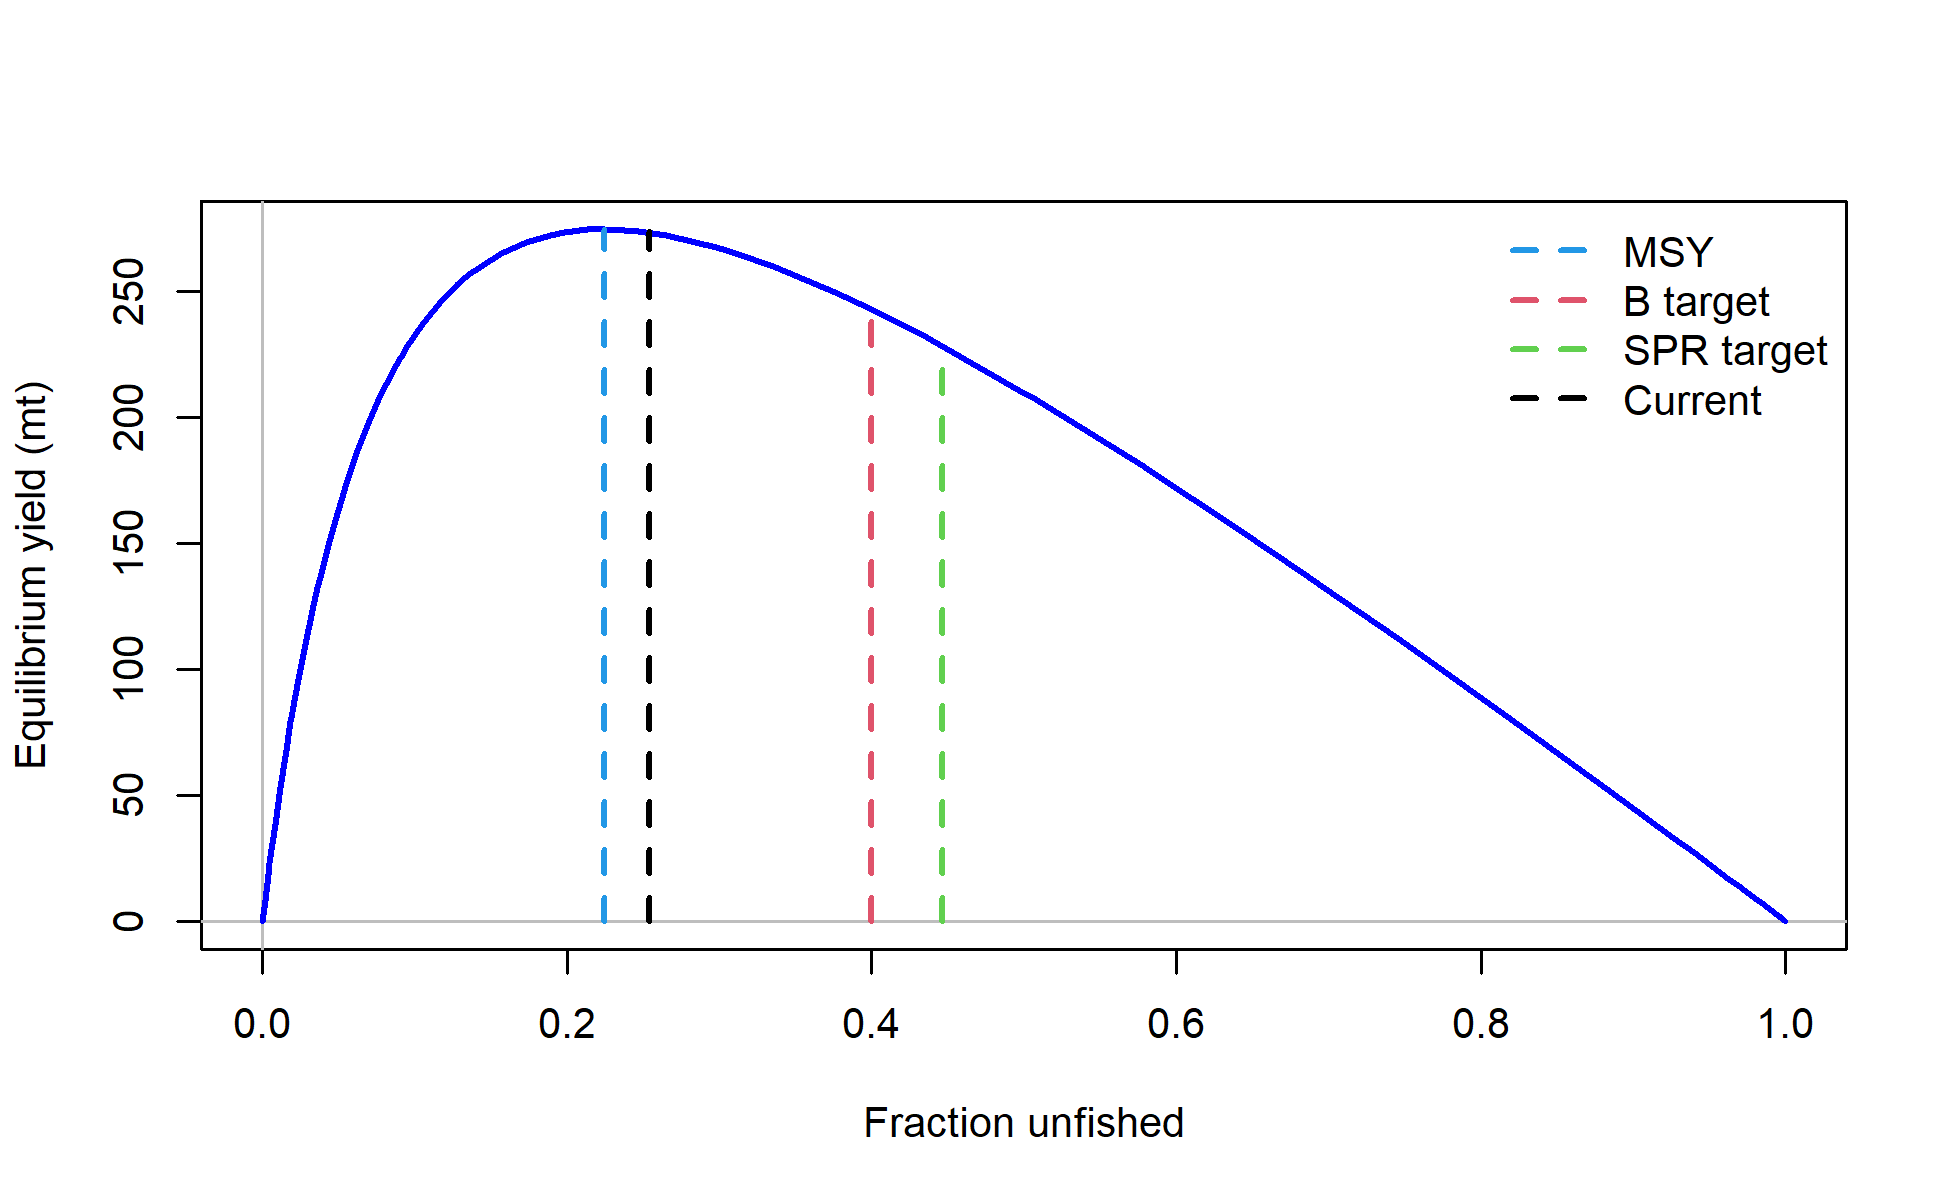
\includegraphics[width=1\textwidth,height=1\textheight]{C:/Users/Jason.Cope/Documents/Github/Sebastes_melanops_WA/Document/models/Reference model/plots/yield2_yield_curve_with_refpoints.png}
\caption{Equilibrium yield curve for the base case model. Values are based on the 2020 fishery selectivities and with steepness fixed at 0.80.\label{fig:es-yield}}
\end{figure}

\begingroup\fontsize{10}{12}\selectfont
\begingroup\fontsize{10}{12}\selectfont

\begin{longtable}[t]{r>{\centering\arraybackslash}p{2cm}>{\centering\arraybackslash}p{2cm}}
\caption{\label{tab:referenceES}Summary of reference points and management quantities, including estimates of the  95 percent intervals.}\\
\toprule
 & Estimate & Interval\\
\midrule
\endfirsthead
\caption[]{Summary of reference points and management quantities, including estimates of the  95 percent intervals. \textit{(continued)}}\\
\toprule
 & Estimate & Interval\\
\midrule
\endhead

\endfoot
\bottomrule
\endlastfoot
Unfished Spawning Output & 943.88 & 867.65-1020.10\\
Unfished Age 0+ Biomass (mt) & 8704.38 & 7999.16-9409.60\\
Unfished Recruitment (R0) & 1959.43 & 1801.19-2117.67\\
Spawning Output (2023) & 426.15 & 251.53-600.77\\
Fraction Unfished (2023) & 0.45 & 0.30-0.60\\
\underline{Reference Points Based on SB40\%} & \\
Proxy Spawning Output SB40\% & 377.55 & 347.06-408.04\\
SPR Resulting in SB40\% & 0.46 & 0.46-0.46\\
Exploitation Rate Resulting in SB40\% & 0.05 & 0.05-0.05\\
Yield with SPR Based On SB40\% (mt) & 293.52 & 269.82-317.22\\
\underline{Reference Points Based on SPR Proxy for MSY} &  & \\
Proxy Spawning Output (SPR50) & 421.11 & 387.11-455.12\\
SPR50 & 0.50 & -\\
Exploitation Rate Corresponding to SPR50 & 0.05 & 0.05-0.05\\
Yield with SPR50 at SB SPR (mt) & 275.88 & 253.60-298.17\\
\underline{Reference Points Based on Estimated MSY Values} &  & \\
Spawning Output at MSY (SB MSY) & 212.51 & 195.32-229.69\\
SPR MSY & 0.30 & 0.30-0.30\\
Exploitation Rate Corresponding to SPR MSY & 0.08 & 0.08-0.08\\
MSY (mt) & 332.18 & 305.38-358.98\\*
\end{longtable}
\endgroup{}
\endgroup{}


\clearpage

\hypertarget{management-performance}{%
\subsection*{Management performance}\label{management-performance}}
\addcontentsline{toc}{subsection}{Management performance}

Removals have been below the equivalent ABC-ACL since the prior assessment (Table ES-6), but those specified ABCs from the 2007 assessments are higher than those coming from the current assessment models. Removals over the last few years have or may have exceeded the newly estimated ABC-ACL values in some years. The differences in the treatment of natural mortality between the previous and current assessments are the biggest reason for this discrepancy.

Exploitation on Black Rockfish increased starting around 1960 and reached a high in the early 1990s. Since that time, catch has mostly fluctuated between 5 and 10 mt per year, with some years exceeding 10 mt, particularly in the last 4 years. The last ten years of the vermilion rockfish component acceptable biological catch (ABC) and annual catch limit (ACL) (which are equivalent) of the Minor Shelf Rockfish North Complex has been set, by definition, below the overfishing limit (OFL) (Table \ref{tab:ofl-es}). The Black Rockfish component OFL for this Complex has been exceeded by the Oregon removals in the most recent 4 years.

\begingroup\fontsize{10}{12}\selectfont
\begingroup\fontsize{10}{12}\selectfont

\begin{longtable}[t]{l>{\raggedright\arraybackslash}p{1.83cm}>{\raggedright\arraybackslash}p{1.83cm}>{\raggedright\arraybackslash}p{1.83cm}>{\raggedright\arraybackslash}p{1.83cm}>{\raggedright\arraybackslash}p{1.83cm}}
\caption{\label{tab:ofl-es}The OFL, ABC, ACL, landings, and the estimated total mortality in metric tons.}\\
\toprule
Year & OFL & ABC & ACL & Landings & Est. Total Mortality\\
\midrule
\endfirsthead
\caption[]{\label{tab:ofl-es}The OFL, ABC, ACL, landings, and the estimated total mortality in metric tons. \textit{(continued)}}\\
\toprule
Year & OFL & ABC & ACL & Landings & Est. Total Mortality\\
\midrule
\endhead

\endfoot
\bottomrule
\endlastfoot
2011 & 11.1 & 5.6 & 5.6 & 70.6 & 70.6\\
2012 & 11.1 & 5.6 & 5.6 & 64.5 & 64.5\\
2013 & 9.7 & 8.1 & 8.1 & 68.6 & 68.6\\
2014 & 9.7 & 8.1 & 8.1 & 73.6 & 73.6\\*
\end{longtable}
\endgroup{}
\endgroup{}

\hypertarget{unresolved-problems-and-major-uncertainties}{%
\subsection*{Unresolved problems and major uncertainties}\label{unresolved-problems-and-major-uncertainties}}
\addcontentsline{toc}{subsection}{Unresolved problems and major uncertainties}

The most significant uncertainty for all models is the treatment and value of natural mortality and the form of fleet selectivity (e.g., length-based asymptotic vs.~age-based dome-shaped selectivity). Data-driven selection between the extreme ``kill'' (using a ramping of M) or ``hide'' hypotheses are not currently resolvable. The current California and Washington base models instead use a form of the ``kill'' hypothesis by not implementing the age-based selectivity (``hide'' hypothesis) and estimating female and male natural mortality, thus avoiding a fixing natural mortality as was necessary in the Oregon model. The Oregon model also contained a step in female natural mortality, a specification not used in the California or Washington models. Another important issue is the highly uncertain historical time-series of removals in all states, which needs further consideration. The development of fishery-dependent indices of abundance still requires further attention. Steepness, while fixed, is still highly uncertain for rockfishes and currently is mismatched to the MSY proxy. And while the steepness profile shows low sensitivity in several derived quantities, steepness strongly defines the yield capacity of stocks, and therefore could cause major uncertainty in the recommended management quantities. Stock structure and its relationship to the current political/management boundaries are also not fully understood, both within U.S. jurisdiction and between the U.S. and Canada. While this is a common challenge faced in most west coast stock assessments, further improvement on this topic will likely rely on black rockfish-specific data.

\hypertarget{scientific-uncertainty}{%
\subsection*{Scientific uncertainty}\label{scientific-uncertainty}}
\addcontentsline{toc}{subsection}{Scientific uncertainty}

The model-estimated uncertainty around the 2015 spawning biomass was \(\sigma\) = 0.01 and the uncertainty around the OFL was \(\sigma\) = 0.01. This is likely an underestimate of overall uncertainty because of the necessity to fix some parameters such as steepness, as well as a lack of explicit incorporation of model structural uncertainty.

\hypertarget{harvest-projections-and-decision-table}{%
\subsection*{Harvest Projections and Decision Table}\label{harvest-projections-and-decision-table}}
\addcontentsline{toc}{subsection}{Harvest Projections and Decision Table}

Black rockfish assessments for California and Washington have a preliminary distinction as category 1 stock assessments, thus harvest projections and decision tables are based on using P\emph{=0.45 and sigma = 0.36, resulting in a multiplier on the OFL of 0.956. The Oregon black rockfish assessment is a category 2 assessment, with a P}=0.45 and sigma = 0.72 with a multiplier of 0.913 applied to the OFL. These multipliers are also combined with the rockfish MSY proxy of FSPR=50\% MSY and the 40-10 harvest control rule to calculate OFLs, ABCs and ACLs. Projections for each state are provided in Table ES-7 to Table ES-9.

Uncertainty in management quantities for the base model of each state was characterized by exploring various model specifications in a decision table. Initial exploration included natural mortality and steepness values, and uncertainty in historical trawl catches for the WA and CA models. OR explored the scale factor coming from the value of the tagging catchability (Q) parameter, as well as M values. For the CA and WA models, there was very little sensitivity to steepness and trawl catches, but natural mortality produced sensitive results of predicted population scale and status. Discussion with the STAR panel resulted in high and low states of nature +/- 0.03 from the base case natural mortality values for females and males. High and low catch streams (rows) were determined by the forecasts, as described above, for each state of nature. Thus the low catch stream is based on the forecast from the low state of nature. The OR model demonstrated little sensitivity to M, but high sensitivity to the tagging survey Q. High and low states of nature, respectively, were based on a fixed tag of Q = 0.125 and Q estimated by the model. Resultant decision tables are provided in Table ES-10 to Table ES-12.

A ten year (2023-2032) projection of the reference model with removals in 2021 and 2022 provided by the Groundfish Management Team for each fleet under the category 1 (sigma=0.5) time-varying buffer using \(P^*\) = 0.45 and 40-10 ABC control rule is provided in Table \ref{tab:project_ES}.

\begingroup\fontsize{9}{11}\selectfont
\begingroup\fontsize{9}{11}\selectfont

\begin{longtable}[t]{c>{\centering\arraybackslash}p{1.38cm}>{\centering\arraybackslash}p{1.38cm}>{\centering\arraybackslash}p{1.38cm}>{\centering\arraybackslash}p{1.38cm}>{\centering\arraybackslash}p{1.38cm}>{\centering\arraybackslash}p{1.38cm}>{\centering\arraybackslash}p{1.38cm}}
\caption{\label{tab:project_ES}Projections of potential OFLs (mt), ABCs (mt), the buffer (ABC = buffer x OFL), estimated spawning biomass, and fraction unfished for Oregon portion of the vermilion stock. The North of 40°10'N OFL and ABC for 2021 and 2022 are included for comparison.}\\
\toprule
Year & OFL 40°10'N & ACL 40°10'N & Predicted OFL & ABC Catch & Buffer & Spawning Output & Fraction Unfished\\
\midrule
\endfirsthead
\caption[]{Projections of potential OFLs (mt), ABCs (mt), the buffer (ABC = buffer x OFL), estimated spawning biomass, and fraction unfished for Oregon portion of the vermilion stock. The North of 40°10'N OFL and ABC for 2021 and 2022 are included for comparison. \textit{(continued)}}\\
\toprule
Year & OFL 40°10'N & ACL 40°10'N & Predicted OFL & ABC Catch & Buffer & Spawning Output & Fraction Unfished\\
\midrule
\endhead

\endfoot
\bottomrule
\endlastfoot
2021	&	9.70	&	8.10	&	13.01	&	12.96	&	1.00	&	21.37	&	0.73\\
2022	&	9.70	&	8.10	&	13.35	&	12.96	&	1.00	&	21.53	&	0.73\\
2023	&	-	&	-	&	13.41	&	12.54	&	0.94	&	21.75	&	0.74\\
2024	&	-	&	-	&	13.29	&	12.36	&	0.93	&	21.85	&	0.75\\
2025	&	-	&	-	&	13.03	&	12.06	&	0.93	&	21.74	&	0.74\\
2026	&	-	&	-	&	12.72	&	11.73	&	0.92	&	21.46	&	0.73\\
2027	&	-	&	-	&	12.41	&	11.38	&	0.92	&	21.08	&	0.72\\
2028	&	-	&	-	&	12.10	&	11.05	&	0.91	&	20.65	&	0.71\\
2029	&	-	&	-	&	11.82	&	10.74	&	0.91	&	20.20	&	0.69\\
2030	&	-	&	-	&	11.56	&	10.45	&	0.90	&	19.75	&	0.68\\
2031	&	-	&	-	&	11.31	&	10.18	&	0.90	&	19.33	&	0.66\\
2032	&	-	&	-	&	11.08	&	9.94	&	0.90	&	18.92	&	0.65\\*
\end{longtable}
\endgroup{}
\endgroup{}


The decision table (Table \ref{tab:es-dec-tab}) was constructed using female and male natural mortality to define the low and high states of nature. The multi-parameter likelihood profile was used to find the low (Female M = 0.07092; Male M= 0.06525) and high (Female M = 0.08527; Male M = 0.07845) female and male natural mortality values that produce -log likeliehood values +0.66 units from the reference -log likelihood value. These correspond to the 12.5\% and 87.5\% quantiles (standard quantiles used in west coast decision tables). The catch rows in the table were based on three proposed catch streams: 1. P* = 0.45, sigma = 0.5 2. P* = 0.40, sigma = 0.5 3. An equilibrium catch based on the \(F_{MSY}\) proxy using SPR = 0.5.

Across all states of natures and catch streams, vermilion rockfish relative stock size never falls below the target relative stock size of 40\%. Both P* approaches lower the stock status from the high relative stock size values, while the \(F_{MSY}\) proxy does not. The mismatch in the corresponding steepness value (\(h=0.6\)) that matches MSY at SPR = 0.5 with the steepness value in the stock assessment (\(h=0.72\)) that correpsonds to an MSY SPR of 0.35 explains why this constant catch will maintain the stock at very high relative stock status levels.

\clearpage

\begingroup\fontsize{9}{11}\selectfont
\begingroup\fontsize{9}{11}\selectfont

\begin{longtable}[t]{l>{\raggedright\arraybackslash}p{0.08\linewidth}>{\raggedright\arraybackslash}p{0.08\linewidth}>{\raggedright\arraybackslash}p{0.1\linewidth}>{\raggedright\arraybackslash}p{0.09\linewidth}>{\raggedright\arraybackslash}p{0.1\linewidth}>{\raggedright\arraybackslash}p{0.09\linewidth}>{\raggedright\arraybackslash}p{0.1\linewidth}>{\raggedright\arraybackslash}p{0.09\linewidth}}
\caption{\label{tab:es-dec-tab}Decision table summary of 10 year projections beginning in 2023 for alternative states of nature based on an axis of uncertainty related to model structure relative to the reference model. Columns range over low (12.5 quantile), mid (reference model), and high states (87.5 quantile) of nature and rows range over different catch level assumptions. The first two years are fixed by the current harvest specifications.}\\
\toprule
\multicolumn{3}{c}{ } & \multicolumn{2}c{low $lnR_0$} & \multicolumn{2}c{Reference Model} & \multicolumn{2}c{High $lnR_0$} \\
\cmidrule(l{3pt}r{3pt}){4-5} \cmidrule(l{3pt}r{3pt}){6-7} \cmidrule(l{3pt}r{3pt}){8-9}
  & Year & Catch & Spawning Output & Fraction Unfished & Spawning Output & Fraction Unfished & Spawning Output & Fraction Unfished\\
\hline
&	2023	&	201	&	352	&	0.39	&	426	&	0.45	&	557	&	0.56\\	
&	2024	&	201	&	348	&	0.39	&	427	&	0.45	&	562	&	0.56\\	
&	2025	&	228	&	343	&	0.38	&	423	&	0.45	&	562	&	0.56\\	
&	2026	&	225	&	335	&	0.37	&	416	&	0.44	&	554	&	0.55\\	
&	2027	&	224	&	331	&	0.37	&	412	&	0.44	&	548	&	0.55\\	
P*=0.4	&	2028	&	224	&	331	&	0.37	&	411	&	0.43	&	543	&	0.54\\	
sigma=0.5	&	2029	&	225	&	33	&	0.37	&	412	&	0.44	&	541	&	0.54\\	
&	2030	&	226	&	340	&	0.38	&	416	&	0.44	&	540	&	0.54\\	
&	2031	&	227	&	346	&	0.39	&	421	&	0.45	&	541	&	0.54\\	
&	2032	&	228	&	354	&	0.39	&	427	&	0.45	&	543	&	0.54\\	
&	2033	&	228	&	361	&	0.40	&	433	&	0.46	&	546	&	0.54\\	
&	2034	&	226	&	368	&	0.41	&	439	&	0.48	&	548	&	0.55\\	
\hline																	
	&	2023	&	201	&	352	&	0.39	&	426	&	0.45	&	557	&	0.56\\	
	&	2024	&	201	&	348	&	0.39	&	427	&	0.45	&	562	&	0.56\\	
	&	2025	&	245	&	343	&	0.38	&	423	&	0.45	&	562	&	0.56\\	
	&	2026	&	241	&	333	&	0.37	&	414	&	0.44	&	552	&	0.55\\	
	&	2027	&	240	&	326	&	0.36	&	407	&	0.43	&	543	&	0.54\\	
P*=0.45	&	2028	&	241	&	325	&	0.36	&	404	&	0.43	&	537	&	0.54\\	
sigma=0.5	&	2029	&	242	&	326	&	0.36	&	404	&	0.43	&	532	&	0.53\\	
	&	2030	&	244	&	330	&	0.37	&	406	&	0.43	&	530	&	0.53\\	
	&	2031	&	245	&	335	&	0.37	&	410	&	0.43	&	529	&	0.53\\	
	&	2032	&	246	&	341	&	0.38	&	414	&	0.44	&	529	&	0.53\\	
	&	2033	&	247	&	347	&	0.39	&	418	&	0.44	&	530	&	0.53\\	
	&	2034	&	248	&	352	&	0.39	&	423	&	0.45	&	531	&	0.53\\	
\hline																	
	&	2023	&	201	&	352	&	0.39	&	426	&	0.45	&	557	&	0.56\\	
	&	2024	&	201	&	348	&	0.39	&	427	&	0.45	&	562	&	0.56\\	
	&	2025	&	279	&	343	&	0.38	&	423	&	0.45	&	562	&	0.56\\	
	&	2026	&	279	&	328	&	0.36	&	409	&	0.43	&	547	&	0.55\\	
Equilibrium	&	2027	&	279	&	317	&	0.35	&	398	&	0.42	&	533	&	0.53\\	
yield	from	&	2028	&	279	&	311	&	0.35	&	390	&	0.41	&	522	&	0.52\\
FMSY	proxy	&	2029	&	279	&	308	&	0.34	&	386	&	0.41	&	513	&	0.51\\
of	SPR=0.5	&	2030	&	279	&	309	&	0.34	&	384	&	0.41	&	507	&	0.50\\
	&	2031	&	279	&	311	&	0.35	&	384	&	0.41	&	502	&	0.50\\	
	&	2032	&	279	&	314	&	0.35	&	386	&	0.41	&	500	&	0.50\\	
	&	2033	&	279	&	317	&	0.35	&	388	&	0.41	&	498	&	0.50\\	
	&	2034	&	279	&	320	&	0.36	&	390	&	0.41	&	497	&	0.50\\*	
\hline
\end{longtable}
\endgroup{}
\endgroup{}


\clearpage

\hypertarget{research-and-data-needs}{%
\subsection*{Research and data needs}\label{research-and-data-needs}}
\addcontentsline{toc}{subsection}{Research and data needs}

Recommended avenues for research to help improve future black rockfish stock assessments:

\begin{enumerate}
\def\labelenumi{\arabic{enumi}.}
\tightlist
\item
  Further investigation into the movement and behavior of older (\textgreater{} age 10) females to reconcile their absence in fisheries data. If the females are currently inaccessible to fishing gear, can we find where they are?
\item
  Appropriate natural mortality values for females and males. This will help resolve the extent to which dome-shaped age-based selectivity may be occurring for each.
\item
  All states need improved historical catch reconstructions. The trawl fishery catches in particular require particular attention. Given the huge historical removals of that fleet in each state, the assessment is very sensitive to the assumed functional form of selectivity. A synoptic catch reconstruction is recommended, where states work together to resolve cross-state catch issues as well as standardize the approach to catch recommendations.
\item
  Identifying stanzas or periods of uncertainty in the historical catch series will aid in the exploration of catch uncertainty in future assessment sensitivity runs.
\item
  The ODFW tagging study off Newport should be continued and expanded to other areas. To provide better prior information on the spatial distribution of the black rockfish stock, further work should be conducted to map the extent of black rockfish habitat and the densities of black rockfish residing there.
\item
  An independent nearshore survey should be supported in all states to avoid the reliance on fishery-based CPUE indices.
\item
  Stock structure for black rockfish is a complicated topic that needs further analysis. How this is determined (e.g., exploitation history, genetics, life history variability, biogeography, etc.) and what this means for management units needs to be further refined. This is a general issue for all nearshore stocks that likely have significant and small scale stock structure among and within states, but limited data collections to support small-scale management.
\end{enumerate}

\vspace{500cm}

\pagebreak
\setlength{\parskip}{5mm plus1mm minus1mm}
\pagenumbering{arabic}
\setcounter{page}{1}
\renewcommand{\thefigure}{\arabic{figure}}
\renewcommand{\thetable}{\arabic{table}}
\setcounter{table}{0}
\setcounter{figure}{0}

\hypertarget{introduction}{%
\section{Introduction}\label{introduction}}

\hypertarget{basic-information}{%
\subsection{Basic Information}\label{basic-information}}

Black Rockfish (\emph{Sebastes melanops}) are an important component of the recreational fisheries in the nearshore waters off central and northern California, Oregon, and Washington, as well as the non-trawl commercial fisheries in California and Oregon. They range as far north as Amchitka and Kodiak islands in Alaska and are considered uncommon south of central California (Milton S. Love, Yoklavich, and Thorsteinson 2002).

A first assessment of Black Rockfish off considered the population off Oregon and California (S. Ralston and Dick 2003) and reviewed the evidence supporting genetic stock structure for Black Rockfish and other rockfish off the U.S. West Coast and concluded that the Oregon and California populations of Black Rockfish are probably not genetically heterogeneous. That assessment treated the Black Rockfish off California and Oregon as a unit stock. Previous assessments of Black Rockfish off Washington (F. R. Wallace, Hoffman, and Tagart 1999; Y. W. Wallace F. R. aand Cheng and Tsou 2007) describe a study of coastal Black Rockfish genetic structure using 10 sampled sites collected from northern California to southern British Columbia t 1995-97. Results of that study support the notion of separate genetic stocks north and south of Cape Falcon. However, a later study (Baker 1999) of Black Rockfish collected from eight sites along the northern Oregon coast concluded that Black Rockfish from north and south of Cape Falcon were genetically very similar.

Although a stock boundary line at the Columbia River seems reasonable for Black Rockfish, both because it is a state fishery management boundary and because the Columbia River plume is likely to be a natural barrier to the north-south exchange of Black Rockfish adults and larvae, the 2007 assessment of Black Rockfish off Oregon and California (Sampson 2007) differed slightly from Ralston and Dick (2003) in placing the northern boundary at Cape Falcon rather than at the Columbia River. The boundary was changed to avoid overlap with the separate northern assessment (Y. W. Wallace F. R. aand Cheng and Tsou 2007) and to simplify the process of assembling historical commercial landings data, which are largely available in terms of Pacific Marine Fisheries Commission (PMFC) statistical areas. The northern boundary of PMFC Area 2C is at Cape Falcon (Figure 1). Given the spatial resolution of the historical commercial fishery data, it is very problematic to estimate the catch of Black Rockfish taken north of Cape Falcon but south of the Columbia River.

During a preliminary workshop in April 2015 (Council 2015), to discuss approaches for assessing Black Rockfish, China rockfish (\emph{S. nebulosus}), and kelp greenling (\emph{Hexagrammos decagrammus}), it was agreed that the assessments for these nearshore species should at a minimum be spatially stratified with boundaries at the CA/OR border (42\textdegree00' N latitude) and the OR/WA border (46\textdegree16' N latitude). Such a spatial stratification would be consistent with two ideas: (a) these nearshore species do not exhibit much adult movement and (b) exploitation and management histories have varied significantly among the three states. Together these features would likely create appreciable state-to-state differences in age composition for each of the three species. Stock assessment teams were advised that they could use geographic strata that were finer than the state level if there were data to support such an approach (Figure 1).

At the same nearshore stock assessment workshop, it was agreed that recreational catch histories for the stocks of Black Rockfish should be assembled on the basis of port of landing rather than location of fish capture, even though fishing vessels landing their catches into a port in one state might have captured fish in waters off a neighboring state.

Accounting for location of capture is very problematic for recreationally caught fish and for commercial catches taken with non-trawl types of gear (e.g., hook-and-line), for which there are no or very limited logbooks that report fishing location. For these regional assessments the commercially caught Black Rockfish were apportioned to assessment region based on the port of landing, with the exception of trawl caught fish landed into Astoria, OR. Most of these fish were assumed to have been caught off Washington and most of the trawl landings into Astoria were therefore included with the catch history for the Washington assessment region. Details are provided below in Section 2.1.1.1 The PacFIN Era (1981 to 2014).

\hypertarget{life-history}{%
\subsection{Life History}\label{life-history}}

Adults tend to occur in schools over rocky structure at depths less than 40 fathoms, and sometimes feed actively on or near the surface. They feed on a wide variety of prey including zooplankton, krill, mysids, sand lance, and juvenile rockfish, and are subject to predation by lingcod and marine mammals (Milton S. Love, Yoklavich, and Thorsteinson 2002).

Although tagging studies have documented some individuals moving long distances (several hundreds of miles), the vast majority of recaptured individuals were found close to the areas of initial capture and tagging (Culver 1987; Ayres 1988; F. R. Wallace et al. 2010; Starr and Green 2007). Results from a 2004-05 study off Newport, OR of 42 Black Rockfish implanted with acoustic tags indicated that all but seven fish remained within range of a 3 x 5 km array of acoustic receivers during one full year of monitoring and had relatively small home ranges that did not vary seasonally (S. J. Parker et al. 1995). Green and Starr (2011) report similar findings from a study in Carmel Bay, CA of 23 acoustically tagged Black Rockfish. The extensive Washington state tagging study also supported low movements for most individuals, with some exceptional movements recorded (F. R. Wallace et al. 2010).

Like all members of the genus Sebastes, Black Rockfish have internal fertilization and bear live young approximately two months after insemination. Black Rockfish are quite fecund, with a six-year-old female annually producing about 300,000 embryos and a 16-year-old producing about 950,000 embryos (Bobko and Berkeley 2004). Recent studies have demonstrated that the relative number and quality of larvae increase with age in female Black Rockfish (Berkeley, Chaoman, and Sogard 2004; Hixon, Johnson, and Sogard 2014). Parturition of larvae occurs during winter (Echeverria 1987) and larvae and small juveniles are pelagic for several months to a year (Boehlert and Yoklavich 1983). Settlement occurs in estuaries, tide-pools, and in the nearshore at depths less than 20 m (Stein and Hassler 1989).

Black Rockfish begin recruiting to nearshore fisheries at 3-4 years of age, corresponding to a fork length of about 25-30 cm, and 50\% of females attain maturity at about 6-8 years, corresponding to a fork length of about 38-42 cm. Adult female Black Rockfish grow 3-5 cm larger than males, with a few females attaining fork lengths greater than 55 cm.

\hypertarget{ecosystem-considerations-1}{%
\subsection{Ecosystem Considerations}\label{ecosystem-considerations-1}}

No formal ecosystem considerations have been made given the lack of data for such an undertaking. Differences in growth though time have been considered in the model specification in the Washington model. Though the mechanism is not specified, this could certainly be due to process error driven by environmental conditions.

\hypertarget{historical-and-current-fishery-information}{%
\subsection{Historical and Current Fishery Information}\label{historical-and-current-fishery-information}}

Black Rockfish are harvested by a wide variety of fishing methods including trawling, trolling, and hook-and-line fishing with jigs and long-lines. Although Black Rockfish have never been a dominant component of any commercial fisheries, they are important as incidental catch in the troll fishery for salmon and the troll and jig fisheries for groundfish. With the decline of salmon fishing opportunities in the late 1970s and early 1980s Black Rockfish became a vital target of marine recreational fisheries in Oregon and Washington, especially during periods of restricted or slack fishing for salmon, halibut, and tuna.

Black Rockfish are also an important component of the recreational fisheries in northern California but are of less significance south of Cape Mendocino due to their reduced prevalence compared to other species. Since 1990 annual recreational harvests of Black Rockfish have averaged 229.6 tons off California, 304.4 tons off Oregon, and 272.5 tons off Washington. Commercial annual harvests by non-trawl gear types during the same period averaged 44.6 tons in California, 62.0 tons in Oregon, and 14.7 tons in Washington. Harvests by trawl on average during this period have been less than 19.3 tons annually for all three states combined.

Removal histories have been a significant axis of uncertainty in the past assessments of Black Rockfish. Because of concerns about the effects of initial equilibrium assumptions on the level of depletion estimated in the preliminary base model, the 2003 Stock Assessment Review (STAR) panel worked with the Stock Assessment Team (STAT) to develop a catch history that avoided the need to assume historical catch and equilibrium conditions in the first year of the assessment. The assumed catch reconstruction began in 1946, ramping up from zero in 1945 and all prior years. In hindsight, this may not have been a good assumption, as indicated by the following text from (Cleaver 1965) that describes catches of rockfish from 1941 to 1949 in Oregon.

``The rockfish are caught by otter trawl and long-line gear. The principal species caught by the otter trawl are the Black Rockfish (\emph{Sebastodes melanops}); green or yellowtail rockfish (\emph{S. flavidus}); red or orange rockfish (\emph{S. pinniger}); and rosefish (\emph{S. alutus}). The landings of rockfish (all species) rose rapidly during the war from 1,301,400 pounds in 1941 to a peak of over 17,000,000 in 1945. Subsequently the landings fell rapidly because of decreased demand and leveled off at about 4,000,000 per year in 1949.

Cleaver (1965) also states, in an introductory section on Bottom Fisheries, that the ``otter trawl fishery accounts for at least 95 percent by weight of the bottom fish landings.''

That Black Rockfish is one of only four species that Cleaver (1965) identifies as composing the large landings of rockfish in Oregon (most of which was actually taken off of Washington waters) during WWII suggests that Black Rockfish were not a trivial fraction of the large catches taken during the 1940s. One might also suppose that the otter trawl fishery took a large portion of the landings of Black Rockfish. Cleaver's statements are certainly at odds with the catch reconstruction developed in the previous assessments.

It seems that Black Rockfish were also landed in appreciable quantities in California during the 1940s. Black Rockfish was identified by scientific name as one of the ``half-dozen of the larger and more abundant species {[}that{]} make up over half of the annual California commercial poundage landed'' (Anon. 1949).

A major task for the 2007 assessments of Black Rockfish in was developing a plausible reconstruction of historical landings of Black Rockfish and exploring the consequences of those landings. For the current set of assessments catch histories from the past assessments have been reconsidered. Formal catch reconstructions have been conducted in California (Stephen Ralston et al. 2010) and Oregon (Karnowski, Gertseva, and Stephens 2014), but even those relatively newer attempts were reconsidered in light of contributions from state agencies. For this assessment, Washington provided a first step in an approach to provide a reconstructed historical catch time series for a stock, something needed for all species in the state's waters.

\hypertarget{summary-of-management-history-and-performance}{%
\subsection{Summary of Management History and Performance}\label{summary-of-management-history-and-performance}}

Prior to 2000 the Pacific Fishery Management Council (PFMC or Council) managed the fishery for Black Rockfish as part of the Sebastes complex, with no separate Acceptable Biological Catch (ABC) or Optimum Yield (OY) for Black Rockfish. In 2000 the Council established an ABC of 1,200 mt for Black Rockfish caught north of Cape Mendocino (in the Eureka, Columbia, and Vancouver INPFC statistical areas), but left Black Rockfish south of Cape Mendocino as part of the ``other rockfish'' category. For 2001 through 2003 the ABC for Black Rockfish caught north of Cape Mendocino was 1,115 mt annually, and Black Rockfish south of Cape Mendocino remained part of the ``other rockfish'' category and without a separate ABC or OY.

Regulation of the Black Rockfish fisheries by the PFMC prior to 2004 was accomplished primarily by trip limits for commercial fisheries and bag limit restrictions for recreational fisheries, with different limits applying in different geographic regions (see Table 1 in S. Ralston and Dick (2003)). Some other important regulations include the following.

\begin{itemize}
\tightlist
\item
  1953: California prohibited trawling within three miles of shore.
\item
  1995: The commercial hook-and-line fishing in Washington state waters (0-3 miles) was closed to preserve recreational fishing opportunities and avoid localized depletion; the closure was extended to trawlers in 1999. Oregon established Black Rockfish management areas with reduced daily commercial fishery trip limits in area near ports with large recreational fisheries.
\item
  2000: Black Rockfish began to be managed by the Council as a minor nearshore species. Commercial trip limits were significantly reduced, with specific restrictions applying to Black Rockfish. California instituted seasonal closures for commercial and recreational fisheries inside 20 fathoms, reduced the bag limit for rockfish from 15 to 10 fish, and limited recreational gear to one line with three hooks.
\item
  2002: California adopted a Nearshore Fishery Management Plan and began more active management of nearshore fisheries including the use of seasonal, regional, and depth-specific closures. Oregon adopted an Interim Nearshore Fishery Management Plan in anticipation of increased pressure on nearshore stocks due to reduced fishing opportunities for groundfish in federal waters. Regulations included fishing-sector specific caps on retained harvests, set approximately at the levels attained in 2000.
\item
  2003: The Council established Rockfish Conservation Areas (RCAs) to control catches of overfished rockfish species, and large portions of the shelf were closed to fishing. Differential trip limits were applied north and south of a management boundary at 40\textdegree10' N. latitude for nearshore Sebastes species. Nearshore permittees in California became subject to depth restrictions consistent with the shoreward non-trawl RCA boundary. In California the commercial and recreational fisheries for rockfish were closed early.
\item
  In 2004 and 2005: the sport fishery in Oregon closed in September 2004 due to early attainment of the state's limit for sport-caught Black Rockfish. This was the first time that the sport rockfish fishery in Oregon had not been open all year. In 2005 it closed early again.
\item
  In 2008 the groundfish trawl fishery was closed in Washington from the seaward RCA boundary to the shore north of 48\textdegree10' N. latitude to address increased encounters with yelloweye rockfish and canary rockfish.
\end{itemize}

In recent years California, Oregon and Washington regulations for the marine sport fisheries, which has been the major source of mortality on Black Rockfish, have become quite complicated and variable through time. Tools for regulating the sport fishery include closed areas, depth restrictions, seasonal closures, and bag limits.

California had no recreational bag limit for rockfish until 1990 when a 15 fish per day per angler limit was implemented. In 2000 the limit was reduced to 10 fish per day for each angler's combined bag of rockfish, cabezon and greenling. The fishing season was year-round prior to 2000 and since then has been variable by state management area. There were no gear restrictions prior to 2000. In 2000 anglers were limited to fishing one line with three hooks. Since 2001 they have been restricted to one line with two hooks. There is no minimum size limit for Black Rockfish.

Oregon had no recreational bag limits for marine fishes until 1976 when the state established a 25-fish limit. In 1978 the state established a daily limit of 15 fish for each angler's combined bag of rockfish, cabezon and greenling, which stayed in effect until 1994 when the state established a 10-fish-per-angler daily bag limit specifically for Black Rockfish. Following the early closure of the fishing season for Black Rockfish in 2004, the daily bag limit for Black Rockfish was dropped to 5 fish at the start of 2005 but was increased in-season to 6 fish. The per-angler daily bag limit was 6 fish during 2006 and 2007, 5 fish at the start of 2008 and increased in-season to 6 fish, 6 fish at the start of 2009 and increased in-season to 7 fish where it has remained since.

The goal of Oregon's sport fishery management is to maintain year-round fishing opportunities. In-season adjustments to regulations can be made more restrictive or less restrictive, depending on circumstances and the prospects for early attainment of harvest caps. Seasonal depth restrictions (e.g., inside 30 fathoms April 1 to September 30) are one tool used regularly in recent years to control the fishery, driven largely by the need to avoid bycatch of the primary rebuilding species, canary rockfish and yelloweye rockfish.

Washington had a recreational daily bag limit for rockfish (all species) of 15 fish per day from 1961 to 1991, 12 fish per day from 1992 to 1994, and 10 fish per day from 1995 to 2015. The bag limit for blue rockfish plus Black Rockfish in Marine Area 4B (Neah Bay) has been 6 fish per day since 2010. Fishing seasons for groundfish species are structured to provide year-round fishing opportunities, if possible. Depth restrictions vary by state management area, being more restrictive in the north compared to the south due to higher encounter rates with overfished yelloweye rockfish and canary rockfish. There is no minimum size limit for Black Rockfish.

In 2004 the coastwide ABC established for Black Rockfish was based on the projected yields derived from separate northern {[}wallace\_status\_1999{]} and southern {[}ralston\_status\_2003{]} stock assessments (Table 1). The northern assessment covered the Washington coast and the northernmost portion of Oregon, from Cape Falcon to the WA/OR border at the Columbia River. The southern assessment covered the entire Oregon coast and the California coastline north of Point Arena.

To account for the spatial overlap of the two assessment areas, 12\% of the projected yield from the northern assessment was transferred to the southern region when deriving the coastwide ABC and OY values of 1,315 mt for 2004. State-by-state harvest guidelines were established: 326 mt for California, 450 mt for Oregon, and 540 mt for Washington. A similar approach was taken in 2005 and 2006 and the OY for the area south of the Columbia River was apportioned to harvest guidelines for California and Oregon based on a 42:58 split. The basis for this apportionment is unclear was to support separate harvest guidelines for each state. The catches were apportioned by the average catch share by state in the 1985-2002 period (Council 2004).

In all years when there has been an OY specified for Black Rockfish the estimated catch has been less than the OY, except for 2003 when the estimated coastwide catch exceeded the ABC for north of Cape Mendocino. In 2003 the estimated coastwide catch exceeded the OY by 183 mt for the region north of Cape Mendocino, but 290 mt of this coastwide catch was recreational harvest taken south of Cape Mendocino.

\hypertarget{canadian-and-alaska-fisheries}{%
\subsection{Canadian and Alaska fisheries}\label{canadian-and-alaska-fisheries}}

Black Rockfish is a ``Non-Quota'' species in the Department of Fisheries and Oceans Management Plan, and is not formally assessed in nearshore Canada waters (Fisheries and Canada 2014).

Add Alaska assessment text here.

\hypertarget{data-and-model-inputs}{%
\section{Data and Model Inputs}\label{data-and-model-inputs}}

A description of each data source is provided below (Figure \ref{fig:data-plot}).

\hypertarget{fishery-dependent-data}{%
\subsection{Fishery-Dependent Data}\label{fishery-dependent-data}}

\hypertarget{commercial}{%
\subsubsection{Commercial}\label{commercial}}

\hypertarget{landings}{%
\paragraph{Landings}\label{landings}}

The systems along the U.S. West Coast for monitoring commercial fishery landings in the past did not keep track of the landings of individual rockfish species, largely because many rockfish species have similar market characteristics and therefore were landed as an unsorted mix of species. Black rockfish in particular, which are a nearshore species and much less abundant than many of the offshore rockfish species, were generally landed in mixed-species categories. As a consequence, the historical records do not provide a detailed accounting of the landings of black rockfish. The basic approach taken to develop the landings series in this assessment (as in past assessments) was to apply values for the proportion of black rockfish sampled in mixed-rockfish landings. Data on the proportions of black rockfish are sparse, with the consequence that the landings reconstructions are highly uncertain.

Commercial landings data for the modern era (1981 to present) are taken from the Pacific Fishery Information system (PacFIN), which is a central repository for U.S. West Coast groundfish landings and auxiliary information collected by the three state fishery agencies and other agencies. A description of basic state data collection systems and overview of PacFIN is provided in Sampson and Crone (1997). Updated dockside sampling protocols and data processing procedures for Washington are described in Tsou et al. (2015) and Tsou and Weyland (2015). A variety of sources were used to reconstruct regional landings histories for years earlier than 1981. Comparisons of the commercial catch in each fishery for the current and previous assessments Figure 81.

\hypertarget{the-pacfin-era-1981-to-2014}{%
\subparagraph{The PacFIN Era: 1981 to 2014}\label{the-pacfin-era-1981-to-2014}}

The PacFIN system provides estimates of commercial fishery rockfish landings by species for those strata (year, quarter, port, area, gear type, condition {[}alive or dead{]}, and market category) that have species composition data available to apportion the landings to species. For the commercial fisheries in California the source of the information provided to PacFIN is the CalCOM database, which is the repository for commercial groundfish market sample data managed by the California Cooperative Groundfish Survey (Pearson et al.~2008). In either system, when no species composition data are available, the system reports the landings as the nominal species or as the mixed-species category that it was sold as (e.g., small rockfish), depending on how the landings were originally reported. The amount of unspecified rockfish that cannot be apportioned to species varies by year, area, and gear type. In many instances the landings of unspecified rockfish reported by PacFIN are quite substantial.

Although the separate geographic assessments by state region would ideally have strict geographic separation of landed catch to the location of capture, this is not possible to accomplish because information on the fishing location is generally unavailable. Until recently logbooks that report area of capture were only available for landings by the groundfish trawl fleet. Oregon has required a logbook for commercial vessels participating in its nearshore fishery since 2004. At the same nearshore stock assessment workshop (Council 2015) it was agreed that catch histories for black rockfish stocks should be assembled on the basis of port of landing rather than location of fish capture, based on the assumption that neighboring state would catch approximately equal amounts from off each other's waters. The one exception to this ``port-of-landing equals the state-of-capture rule'' is for trawl-caught fish landed at Astoria, OR, the vast majority of which were caught in waters off Washington.

Staff from the Oregon Department of Fish and Wildlife (ODFW) used species composition samples collected during 1976 to 1993 to conduct an analysis of the spatial distribution of black rockfish landed at Astoria, OR. Astoria is the northernmost port in Oregon and is located near the mouth of the Columbia River, which forms the boundary between Oregon and Washington. The aggregate proportion of black rockfish expanded pounds that were taken north of the Columbia River (i.e., from waters off Washington) was 98.6\%. This percentage was applied to all historical trawl landings of rockfish at Oregon's Columbia River District ports prior to 1976.vNon-trawl landings into Astoria were assumed to have been caught from Oregon waters.

Starting in 1994 black rockfish landed into Oregon were legally required to be sorted and sold in a separate black rockfish market category and were also reported as separate retained catches in the mandatory trawl logbooks. Based on the retained catches reported in the logbooks, the estimated proportion of the trawl-caught black rockfish that were caught from off Washington and landed into Astoria ranged from 65 to 100 percent. These black rockfish are accounted for in the Washington regional assessment (Table 48).

The Washington Department of Fish and Wildlife (WDFW) provided commercial fishery landings based on fish ticket records of black rockfish harvested off Oregon by vessels landing at ports in Washington. Landings were less than 1 mt per year for the period 1971 to 2014; therefore, all landings to Washington ports were assumed to occur in waters off Washington in this assessment.

The landings data series for black rockfish landed in California, Oregon, and Washington during 1981 to 2014 were assembled from three PacFIN or CalCOM data sets. The first data set consisted of direct estimates of black rockfish landings by state (described as BLCK in PacFIN), which the systems derived from fish tickets, species composition estimates, and trawl-logbooks provided by the California Department of Fish and Wildlife (CDFW), the ODFW, and the Washington Department of Fish and Wildlife (WDFW). The second data set consisted of landings of black rockfish that were nominally landed in the black rockfish market category (described as BLK1 in PacFIN) but no direct species composition samples were available to confirm their purity. Prior to 1993, there was no sorting requirement in the states and no explicit market category for black rockfish, which were landed in a mixed-species rockfish category. Starting in 1994, black rockfish landed in Oregon were legally required to be landed and sorted into a separate black rockfish market category. Similar sorting requirements were implemented in 2001 in California and in 2006 in Washington.

The third PacFIN data set (URCK in PacFIN) was derived from landings of rockfish for which species composition sample estimates were unavailable, but which might feasibly contain some black rockfish. This derivation involved applying estimates of the percentages of black rockfish (\%Black) to the landings of unspecified rockfish.

For each regional assessment the final values for annual commercial landings of black rockfish were the sum of the original PacFIN estimates, to which were added the nominal landings of black rockfish (listed as black rockfish on fish tickets but not verified by sampling) and the estimates of black rockfish in the unspecified rockfish landings.

The landings series during the PacFIN era are quite erratic, sometimes exhibiting large variations between years. While these changes could be a true reflection of changing fishing patterns, they may be no more than artifacts of low levels of species composition sampling. A study of the groundfish landings estimates for California (Pearson, Erwin, and Key 2008) evaluated the reliability of species composition sampling for various rockfish species. The study noted that black rockfish are readily misidentified as blue rockfish, that the hook-and-line fishery in California was not well sampled until the 1990s, and that many of the California landings estimates are based on ``borrowed'' data or by treating the black rockfish market category as ``pure''.

\hypertarget{oregon-commercial-fishery-landings-1892-to-2014}{%
\subparagraph{Oregon Commercial Fishery Landings: 1892 to 2014}\label{oregon-commercial-fishery-landings-1892-to-2014}}

The commercial fishery landings data series for Oregon (Table 25) were assembled from four primary sources: 1) PacFIN, as described above; 2) Pacific Marine Fisheries Commission (PMFC) landings data series for 1956 to 1980; 3)Fishery Statistics of the U.S. for 1927 to 1955; and (4) ODFW's Ocean Recreational Boat Survey for 1979 to 2014 (provided by P. Mirick, ODFW). Details regarding the PMFC and Fishery Statistics of the U.S. data series are provided in the 2007 assessment document.

Much of the information underlying the commercial catch reconstruction was assembled from primary sources described above in a database documented in Karnowski et al. (2014). Careful review of the Karnowski et al.~database uncovered some unusual features in the species composition information that underlies the landings reconstruction. For example, during the period 1963 to 1975 the annual \%Black values used in the Karnowski et al. (2014) database varied from 0\% to 100\%, and produced very erratic year-to-year variations in the landings of black rockfish.

Staff from ODFW recommended using an alternative reconstruction of historic landings that was based on a fixed set of PMFC-area specific \%Black values for the time period 1949 to 1975 (2.2\% for area 2A, 4.5\% for 2B, 4.4\% for 2C, and 14.1\% for 3A). There were similar issues with high variability in the \%Black values used in the Karnowski et al.~database for the period 1976 to 1986. For this period staff from ODFW recommended an alternative reconstruction of historic landings based on the following fixed set of PMFC-area specific \%Black values: 0.77\% for area 2A, 0.29\% for 2B, 0.54\% for 2C, and 6.82\% for 3A.

\hypertarget{washington-commercial-fishery-landings-1940-to-2014}{%
\subparagraph{Washington Commercial Fishery Landings: 1940 to 2014}\label{washington-commercial-fishery-landings-1940-to-2014}}

Commercial fishery landings of black rockfish in Washington are compiled from a variety of sources including PacFIN, agency reports, historical fish ticket information and communication with agency personnel (Table 48). Since 1935, commercial fishing vessels have been required to submit a fish receiving ticket (``fish ticket'') for each landing. Rockfish landings from domestic fishers are usually reported in mixed-species market categories, and are routinely sampled for species composition by port samplers. The information required on the ticket and sampling methods have changed through time. Due to these changes, we separated the data into three time periods 1935-1969, 1970-1980, and 1981-present based on the level of detail available in the data for compiling landing history in Washington for this assessment.

\hypertarget{years-1935-to-1969}{%
\subparagraph{Years 1935 to 1969}\label{years-1935-to-1969}}

Although the original paper fish tickets are no longer available for this period, WDFW recently digitized the daily aggregated data from printed reports, to assist in reconstructing the commercial groundfish fishery landings history for Washington. These daily aggregated data reports contain summaries of daily catches for port-groups by gear and area fished. The data are available for 1935 and for 1949-1969, and were used as the basis for the black rockfish catch reconstruction for this time period.

During this period, mixed-species, nominal market categories were typically used for reporting of the aggregated data. Market categories such as ``red rockfish'', ``black rockfish'' (BLK1), and ``unidentified rockfish'' (URCK) are typical on fish tickets during this time, lumping all red colored fish and black colored fish into these categories for reporting. For bottom trawl gears, the BLK1 market category consisted of mostly yellowtail rockfish and silvergrey rockfish (Greg Lippert, pers. comm.). To split the black rockfish landings out of the BLK1 market category, we assumed 10\% of the BLK1 landings were S. melanops (BLCK). We further assumed that no other nominal market categories in the trawl fishery contained S. melanops (see table below).

For the commercial jig and troll fisheries, rockfish were landed in the unidentified rockfish (URCK) market category. No species composition samples are available during this time, so we assumed 85\% of URCK landings were S. melanops, which matches the species composition data from the 1985-1989 commercial jig fishery. These estimates were also supported by interviews with port samplers active during portions of this period. The rockfish caught by troll gears composed of mostly yellowtail and black rockfishes. Wright (1967) reported rockfish species composition of the troll landings by port. We assumed 80\% of URCK caught off central Washington were BLCK and 20\% for northern Washington landings.

\hypertarget{years-1970-to-1980}{%
\subparagraph{Years 1970 to 1980}\label{years-1970-to-1980}}

Original fish ticket data were used for commercial catch estimate during this period. Fishing areas were better defined and reported during this period; there were no longer interstate areas due to the introduction of current management areas, with a boundary line at the OR/WA state border. However, issues with URCK market category remained. Species composition sampling of URCK were conducted for trawl and jig fisheries but not for salmon troll and the ``other gears'' gear types.

To estimate the trawl landings of black rockfish in the category URCK, we applied the current WDFW species composition algorithm by gear, port, and quarter. If no species composition samples were taken during a quarter, we first borrowed annual composition data for the gear/port group. If those data were not available, a coastwide annual composition for the particular gear type was applied. There was no borrowing of composition information across gear groups or years.

The commercial jig fleet operates in nearshore waters and black rockfish is the dominant component of the URCK landing for this gear type. Species composition sampling was not conducted during the 1970-1980 time period. Based on the samples collected in the 1980s, we assumed that black rockfish made up 80\% of the total rockfish landed by the jig fleet. For the troll fishery, the same proportions as for the pre-1970 time period were applied.

Rockfish (URCK) were also landed in small amounts by other commercial fleets, such as fixed gears and salmon troll. The fleets in the 70s and 80s predominantly targeted sablefish and halibut in waters too deep for black rockfish. Port samplers did not recall observing any black rockfish in the fixed gear landings (James Beam and Greg Lippert, pers. comm.). Therefore, we assumed fixed gear landings were negligible. For URCK landed by the salmon troll fleet, the majority of troll landings was yellowtail rockfish with smaller numbers of widow, canary, and black rockfish (Wendy Beeghley and James Beam, pers. comm.). We assumed that 10\% of the troll rockfish landings were black rockfish for 1970-1980.

\hypertarget{years-1981-to-the-present-the-pacfin-era}{%
\subparagraph{Years 1981 to the Present (the PacFIN era)}\label{years-1981-to-the-present-the-pacfin-era}}

Rockfish landings from this period are pulled from the PacFIN table called VDRFD. Landings in this table are the products of nominal landings, as well as area and species compositions. For the remaining URCK in this table, we applied a coastwide annual composition for each gear, as described above. After this step, there are still small amounts of URCK for trawl and setline gears. These landings are not included in this assessment.

For the jig-gear fishery, dockside sampling was conducted by the WDFW Ocean Sampling Program (OSP) during 1985-1991. These species composition data are not available in PacFIN. For landings during 1985-1991 the URCK species compositions were stratified by year and port. For other years, species compositions were stratified by port only. For jig-caught fish landed into Seattle annual species compositions from Neah Bay were applied (Table 49) because there was no port sampling in Seattle. The URCK market category was used until 2000, after which it was replaced by the Slope, Shelf, and Nearshore rockfish market categories. The commercial nearshore fishery was closed in 1999, so starting in 2000 there are negligible black rockfish landings in any market categories. In 2005 mandatory sorting was established for black rockfish, so all black rockfish landed should be recorded on fish tickets in the BLK1 category.

To assign URCK commercial salmon troll landings, we used the same reasoning assumption as applied to earlier periods (see 1970-1980) to assign 10\% of the URCK landed in the salmon troll fishery to black rockfish. After a complete nearshore closure in 1999, black rockfish landings have been negligible.

\hypertarget{foreign-fishery-catches-of-black-rockfish}{%
\paragraph{Foreign Fishery Catches of Black Rockfish}\label{foreign-fishery-catches-of-black-rockfish}}

Rogers (2003) developed catch reconstructions for removals by foreign trawlers operating off the U.S. West Coast during the late 1960s to mid-1970s. Although this study reports that Japanese vessels operating in the Columbia and Eureka statistical areas (Oregon and northern California) caught substantial amounts of black rockfish, with cumulative catches of more than 500 mt over 10 years, it seems very unlikely that foreign vessels could have operated sufficiently close to shore to catch appreciable amounts of black rockfish. This assessment does not include Rogers' estimates of foreign fleet removals of black rockfish.

\hypertarget{recreational-removals}{%
\subsubsection{Recreational Removals}\label{recreational-removals}}

Comparisons of the catch in each recreational fishery for the current and previous assessments are in Figure 81 (OR), and Figure 179 (WA).

\hypertarget{oregon-ocean-boats-1973--2014}{%
\paragraph{Oregon Ocean Boats: 1973 -2014}\label{oregon-ocean-boats-1973--2014}}

To produce total catch estimates, the Oregon Recreational Boat Survey (ORBS) applies catch rates from a subsample of vessels (from dockside interviews) to total effort counts at fine levels of stratification (e.g., by week, port, fishery, and type of boat).

For estimates of landings, catch rates are verified by ORBS biologists. However, estimates of discarded mortality are based on angler-reported data and thus are less certain. To estimate discard mortality, ORBS first estimates the number of discarded fish (by species), to which it then applies stratified mortality rates based on the depth of capture to account for the depth-dependent mortality rates associated with barotrauma (Council 2014). Since the greatest source of black rockfish removals has been from landed catch (typically only 1\% of removals are from discard mortality), there has been a relatively high degree of certainty in sport fishery removals.

Since 2001, ORBS has produced comprehensive year-round estimates of catch and effort for all developed Oregon ports (which are available from RecFIN). However, prior to 2001, ORBS sampling was typically only conducted at major ports during the peak months of sport fishing activity, and no estimates of landed catch were made for unsampled ports and times. Accordingly, ODFW reconstructed historic ORBS estimates of black rockfish to include landed catch from all ports and times (not yet available on RecFIN), as is done in recent years.

The sport reconstruction addressed four spatial and temporal coverage biases identified during an external review of ORBS by the RecFIN Statistical Subcommittee ( et al. 2000): 1 ``Major ports'' that were sampled each year were not sampled during the winter months 2 ``Minor ports'' were not sampled at all during some years 3 effort counts for private boats excluded afternoon and night trips 4 undeveloped launch sites were never sampled (e.g., beaches).

The sport reconstruction utilized ratio estimators, based on years with complete sampling, to expand catches from years with partial sampling. For instance, the contribution of winter catch to total catch during years with complete sampling was used to the expand catches for years with missing winter catch. Similarly, the contribution of catch from a minor port to that of the major ports during years with complete sampling was used to expand catches of years that the minor port was not sampled. The reconstructed catch and effort estimates for ocean boats ramp up in a near linear fashion from the beginning of the time series in 1973 to an initial peak in 1984. Attempts to estimate ocean boat catch prior to 1973 by fitting a linear function to this initial ramp up resulted in negative catch for 1972, therefore the ocean boat fishery was assumed to have started in 1973. This comports well with anecdotal information on the early years of the ocean boat fishery, but is in contrast to the treatment of shore based and estuary boat fisheries described below.

\hypertarget{oregon-estuary-boats-and-shore-1915-2014}{%
\paragraph{Oregon Estuary Boats and Shore: 1915-2014}\label{oregon-estuary-boats-and-shore-1915-2014}}

Since ORBS has only produced estimates of catch and effort for the ocean boat fishery, estimates of historic black rockfish removals from the estuary boat and shore fisheries were obtained from MRFSS.

Both MRFSS and ORBS were similar in that a dockside angler intercept survey component was used to obtain catch rates. However, MRFSS used a random-digit phone survey to estimate total effort, whereas ORBS used visual counts to estimate private boat effort (i.e., of vessels crossing the ocean bar or trailer counts) and obtained a census of charter effort via logbooks.

Although MRFSS had comprehensive spatial and temporal coverage, MRFSS estimates were determined to be biased during the same external review that identified ORBS biases ( et al. 2000).

The first bias was inclusion of freshwater fishing trips in effort counts for marine fisheries that caused the estimates of trips by boat (and presumably also shore-based trips) to be overestimated by 17\%. Specifically, trips from zip codes non-adjacent to the ocean were being recorded as marine trips in the phone survey. Accordingly, the reconstruction applied a scaling factor to both the shore and estuary boat estimates to remove the freshwater bias.

The second MRFSS bias was an area bias for the boat estimates, whereby ocean boat landings were overestimated by 23\% which led to an underestimation of landings by estuary boats. Although MRFSS estimates of boat catch (by boat type) were not stratified by area, the total (coastwide) estimates were partitioned to inland and ocean areas based on ratios observed in the dockside survey (e.g., if 35\% of sampled catch was from the ocean, then 35\% of total catch was assigned to ocean boats).

In order for these area-partitioned estimates to be correct, the MRFSS dockside samples would have had to been representative; however, it was determined that MRFSS had oversampled the central and southern parts of Oregon, with a greater proportion of ocean trips, than to the north, with a great proportion of estuary trips. Accordingly, another scaling factor was applied to the estuary boat estimates to account for this boat area bias (this bias did not affect the estimates for the shore fishery).

In addition to using scaling factors to account for MRFSS biases --- note that the two biases nearly cancel each other for estuary boats \&mdash the reconstruction also corrected errors in weights of individual fish that were used to covert estimated number of fish (the measure produced by MRFSS) to metric tons. While there were a few clear errors for black rockfish (e.g., a 962 mm, 14 kg fish), these had far less relative effect on total removals than occurred for kelp greenling (where the erroneous 91 kg fish doubled the removals for the shore mode in 1981).

Finally, the reconstruction extrapolated landings for years --- outside the scope of MRFSS coverage (i.e., 1915-1980, 2005-current). For years prior to 1980, fishing license sales, the only Oregon auxiliary data source found to be directed related to fishing, was used to scale historic black rockfish landings. This extrapolation based on Oregon fishing license sales followed the same pattern as observed in the California sport fishery reconstruction for the shore and skiff fisheries (Stephen Ralston et al. 2010). For missing years during the modern era (2005-present), a simple linear trend of the landings from 1980-2005 was used, which also followed the same trajectory as seen with recent license sales (mostly flat, but slightly decreasing).

\hypertarget{washington-sport-fishery-removals-1940-to-2014}{%
\paragraph{Washington Sport Fishery Removals: 1940 to 2014}\label{washington-sport-fishery-removals-1940-to-2014}}

The Washington recreational catch history of black rockfish was reconstructed using several direct and indirect records of black rockfish catch (Table 50). All primary sources report catch in numbers of fish. As sources have been modified and re-evaluated, a completely new catch reconstruction for Washington was developed for this assessment. The following main sources were used in the reconstruction to get numbers of landed black rockfish:

\begin{enumerate}
\def\labelenumi{\arabic{enumi}.}
\tightlist
\item
  Years 1990-2014: Washington Ocean Sampling Program (OSP) boat based angler survey. Monthly catch and effort estimates were based on an expansion procedure that uses a complete count of vessels leaving or entering a port and dockside angler interviews. Dockside interview collects information on number of anglers, catch area, and target species for all sampled trips. Shore-based fishing, other than major jetties (e.g., the north jetty at the mouth of the Columbia River), is not sampled and is considered a negligible mode for catching black rockfish in Washington. Sampling and effort counts occur mainly from April to October. Winter fishing is also considered negligible.
\item
  Years 1967, 1975-1986: Published catch from historical sport catch report series by the Washington Department of Fisheries.
\item
  Years 1987-1989: The RecFIN estimates were initially considered to supplement these missing years, but the reported values of numbers or black rockfish caught were half the numbers reported in the adjacent years in the published catch records and the estimated in the OSP. The average value from years 1984-1986 and 1990-1992 were instead used in an interpolation of estimated numbers of black rockfish caught in 1987-1989.
\item
  Years 1950-1966, 1968-1974: Ratio of total rockfish to salmon catch. Buckley (1965) and WDFW (pers. comm.) reported the number of total rockfish caught relative to the number of salmon. This ratio was used to predict total number of rockfishes for the missing years (Figure 177). Data from Buckley (1965) showed black rockfish comprised approximately 60\% of total rockfish landings in 1964 and 1965. This ratio was applied to the predicted total rockfish estimates to derived black rockfish estimates.
\item
  Years prior to 1950: The resultant values of estimated black rockfish catches during 1950-1974 were used to predict values before 1950 (Figure 178). Only year 1949 showed a positive catch estimate, so it was the final year of predicted catch.
\end{enumerate}

Because the catch was reported in numbers, average weights were used to expand numbers to biomass by year in two ways

\begin{enumerate}
\def\labelenumi{\arabic{enumi}.}
\tightlist
\item
  Years 1979-2014: Average weights converted from lengths (see Section 2.1.4.4 for source of length-weight relationship) from the OSP database were available (except for 1989, which used the average of years 1980-1989).
\item
  Years prior to 1979: The value from 1979 was extended backwards to all previous years. 1979 and 1980 values were very different from the rest of the time series (larger sizes), so it was reasoned older years would be more similar to the adjacent years than other, more recent years. Annual numbers of black rockfish were multiplied by yearly average weights to get the final catch estimates in biomass. Despite this very different approach to catch reconstruction, the final results did not differ greatly from the 2007 assessment (Figure 20).
\end{enumerate}

\hypertarget{alternate-historical-catch-series}{%
\paragraph{Alternate Historical Catch Series}\label{alternate-historical-catch-series}}

The exploration of alternative removal histories was limited before, during and after the STAR panel. After consulting with state representatives it was apparent that more formal catch history reconstructions with the intent on characterizing stanzas of catch uncertainty is generally needed to specify alternative catch histories that reflect the underlying uncertainty in the catch reconstructions. Sensitivities to 50\% and 150\% catch times series, as well as using the former catch history in the Washington model were explore and demonstrated little sensitivity to such changes. More work in the future is thus needed to formalize either alternative catch series or explicitly incorporating catch uncertainty into model specification.

\hypertarget{estimated-discards}{%
\subsubsection{Estimated Discards}\label{estimated-discards}}

In the previous assessment, commercial discards were not accounted for due to the information provided by the West Coast Groundfish Observer Program (WCGOP) at that time, showing about a 1\% discard rate in their survey. We evaluated the WCGOP estimates of black rockfish discards from 2002-2013, which showed a total of 32.2 mt in estimated discards and total landings of 2042.5 mt coastwide, resulting in a rough discard rate estimate of 1.58\%. This amount of discards was included in the CA HKL non-live fishery landings, going back to 1916, and in the OR HKL non-live fishery landings to 1892. Given the minimal amount of discards, no further depth-dependent mortality estimates were evaluated for Oregon and California and this discard rate was added to the total commercial removals. Parker et al (2006) concluded that semi-pelagic, vertically mobile species, such as black rockfish, show less barotrauma; hence these estimates could be slightly overestimated.

Estimates from the ORBS program of discards of black rockfish in the Oregon sport fishery, based on data collected by observers on charter boat trips, also indicated low levels of discarding. This assessment assumes a discard rate of 0.9\% in the sport landings, which is the average of the RecFIN discard estimates in recent years, and this rate is calculated per year and added to the total.

Washington recreational discard estimates were not available until 2002. Numbers of discarded-by-depth black rockfish were estimated using the same catch expansion algorithm for landed catch. Surface release mortalities adopted by the Groundfish Management Team (GMT) in their death-by-depth matrix (11\%, 20\%, 29\%, and 63\%) were then applied to the number of release black rockfish for each of 4 release depth bins (0-10 fm, 11-20 fm, 21-30 fm, and \textgreater30fm), respectively. Total dead released black rockfish were then summed across each depth bin. The average weights of discards were assumed to be the same as the average weights of landed and multiplied by the number of released dead to get total dead in metric tons. For pre-2002 release, proportions of releases based on a ratio estimator using 2003-2007 data were applied. For the split between charter and private vessels, the same algorithm used for splitting retained catch was applied. The overall average discard rate in the recreational fisheries was 1.37\%. There was no information on Washington commercial discards, so the rate of 1.37\% (same as the historical recreational discards) was also applied to the entire commercial time series. This low rate was similar to discard rates estimated in the other states.

\hypertarget{size-and-age-composition-data}{%
\subsection{Size and Age Composition Data}\label{size-and-age-composition-data}}

Fish length measurements, primarily from the recreational fishery, are one of the major sources of data for this assessment. Length composition data from the commercial fisheries in Oregon and California were also included, as were some age composition data from the commercial and recreational fisheries in Oregon.

A large proportion of the length composition data were from the Marine Recreational Fishery Statistics Survey (MRFSS), which is a federally funded program operating since 1980 that collects information on the marine sport fisheries. The MRFSS program includes an intercept survey in which sport anglers are interviewed as they return from fishing trips, and where samplers can identify and measure the retained catches. The MRFSS sampling is intended to cover all forms of marine recreational fishing, including shore-based activities from beaches, jetties, and piers. In contrast the ORBS program that operates only in Oregon interviews and samples anglers operating from boats. The MRFSS length data, which are housed in the RecFIN database, generally do not indicate the sex of individual fish that were measured. Similarly, the length data collected by the ORBS program does not generally indicate gender. In Oregon, a separate and independent sampling program from ORBS, the Marine Non-Salmonid Recreational Fishery Study (MNSRFS), collects length, age and gender data from recreational anglers operating from boats. The length and age data collected by the MNSRFS program are the only recreational data used in the assessment where gender is recorded.

\hypertarget{length-and-age-sample-sizes}{%
\subsubsection{Length and Age Sample Sizes}\label{length-and-age-sample-sizes}}

The level of commercial fishery sampling for black rockfish has been erratic, with almost no samples taken in Oregon until the early 1990s (Figure 80). In California there was a shift from trawl to non-trawl samples, which in part reflects the growing importance of hook-and-line fishing in the nearshore areas and the development of a live-fish fishery. Sampling of the recreational fisheries in Oregon and California by the MRFSS program has been reasonably consistent except for the hiatus during 1990-92 when the program was not funded. The standard MRFSS sampling program stopped in 2003 in Oregon and in 2004 in California, around which time the states assumed larger roles in sampling their recreational fisheries. This resulted in some loss of continuity in the sampling processes.

\hypertarget{multinomial-sample-sizes}{%
\paragraph{Multinomial Sample Sizes}\label{multinomial-sample-sizes}}

Initial input values for the multinomial samples sizes determine the relative weights applied in fitting the annual composition data within the set of observations for each fishery. The initial input values in this assessment were based on the following equation developed by I. Stewart and S. Miller (NWFSC), and presented at the 2006 Stock Assessment Data and Modeling workshop. Neff = Ntrips + 0.138 * Nfish if Nfish/Ntrips \textless{} 44 Neff = 7.06 * Ntrips if Nfish/Ntrips ? 44

Tuning of the assessment model involved multiplying the input sample sizes for each fishery by an adjustment factor to achieve a better balance between how well the model fit the set of composition data and how well it should have fit the data given the sample sizes underlying the data.

\hypertarget{length-compositions}{%
\paragraph{Length Compositions}\label{length-compositions}}

The length data for the assessment model were tabulated into 2-cm length bins ranging from 10 cm to 64 cm, with accumulator bins at each end.

The length composition data indicate some general differences between the three fishery types, with the trawl fisheries producing the largest fish, the recreational fisheries producing the smallest fish, and the non-trawl fisheries producing fish of intermediate length. There is little evidence in any of the length composition data of distinct modes or successions of modes from one year to the next that might represent strong year-classes.

The recreational fishery length composition data from Oregon are generally quite symmetrically distributed, whereas the recreational fishery length composition data from California are often quite asymmetric, with an extended shoulder having modest numbers of large fish. However, the data for the first few years of the California series are similar in general shape to the Oregon recreational length composition data.

Sample length composition data from the California sport fishery for 1999 and 2000 were excluded from the assessment model because they had very narrow distributions and were extremely different from adjacent years. Close examination of the raw data did not indicate any obvious reason for the odd appearance of these length compositions.

\hypertarget{oregon-length-compositions}{%
\subparagraph{Oregon Length Compositions}\label{oregon-length-compositions}}

Commercial

The biological data for the commercial fishery were extracted from PacFIN on April 24th, 2015. These data are from trawl and non-trawl (hook-and-line) dead and live-fish fisheries from ports south of Astoria. The PacFIN dataset contains records for Oregon landings into Astoria; however, these are believed to have been landed in Washington waters and are used in the Washington model. Length composition data are reported either in fork length or total length (Table 27). Fork lengths are preferred; where they are missing the total length is used. These data are expanded to reduce the effect of non-uniform sampling effort. The expansions are by weight, catch/sampled catch; first on a per-trip level, and then on a per-year, per-fishery level. Expansion factors have a minimum value of 1, and are capped at their 90th percentile value. The final sample size is the product of the two expansion factors, which is then capped at its 90th percentile value. The data were stratified by gender and fishery (Table 27). The final sample sizes were stratified and summed by length bin (10 cm to 60 64 cm bins, 2 cm in width), and an effective sample size is computed from the number of trips and number of fish each stratum represents, according to the Stewart and Miller method for multinomial fishery data (See page 56). A small number of unsexed fish were present in the data; as these did not represent a distinct length distribution, they were excluded from the model.

Recreational

Recreational length composition samples for Oregon were obtained and considered from 3 sources: RecFIN, ODFW-ORBS, and independent ODFW length-age sampling. For 1980-1989 and 1993-2003, the MRFSS program collected unsexed individual fish lengths for all modes (MM, BB, CPFV and PR) from both ocean and inland (estuary) areas. From 1980-1989, MRFSS collected total lengths, but after a hiatus from 1990-1992, the renewed MRFSS program began collecting fork lengths. RecFIN provides a species-specific total length to fork length conversion, which was used in to standardize all MRFSS length data to fork length. From 2003-2005, the state managed Shore and Estuary Boat Survey (SEBS) collected fork length data from shore modes in both ocean and inland areas, and from boat modes only in inland areas. MRFSS/SEBS length data were extracted from RecFIN using the sample data query (\url{http://www.recfin.org/sample-data}). Sample sizes and number of trips by year, and fishery used to generate the effective sample size for inputs are shown in Table 29.

From 2001 through the present, the state managed ORBS program has collected unsexed groundfish fork length data from recreational boats, primarily from ocean fisheries but with a handful of samples from boats fishing in inland waters. For this assessment, ORBS length data from 2001-2014 were obtained from ODFW (Table 29). Shore based modes are not sampled by ORBS. A comparison of the ORBS and MRFSS data showed a 2 cm different in average lengths, even though the average lengths by year within each data set change little over time. The reason for this difference is not understood. Given both data sets inform one fishery (the recreational ocean fishery), a block in the selectivity parameters was explored to address this issue, but very similar selectivity values were estimated, so the block was not included in the final base model. Therefore, the effect of this difference is very small in the model, though understanding why it exists (and if it exists in other species) should be looked into further.

From 1978 through the present, ODFW has collected sexed black rockfish length composition data from recreational ocean boat fisheries in conjunction with age structure sampling, independent of both the MRFSS/SEBS and ORBS sampling programs. These collections have been managed under various programs over the years; the current program is known as Marine Non-Salmonid Recreational Fish Studies (MNSRFS), which has existed in its current form since 2005. Collections from 1978 were only from the port of Brookings, and from 1979-1989 were only from the port of Garibaldi. Beginning in 1990, geographic representation improved with sampling occurring in Garibaldi, Newport, and Brookings each year. Beginning in 1994 the port of Charleston was also sampled each year and in 1999, sampling was expanded to include all ports with significant black rockfish landings, although this has been somewhat sporadic in the relatively minor ports (Table X1). No sampling was conducted in 2008. Due to concerns about spatial coverage and aging error in the early part of this dataset, samples from 1996 onward are used in the model. Samples from 1996-1998 are included as a ``Legacy'' dataset. Composition data were used as collected (i.e., not expanded). Sample sizes per trip for the Effective N calculation were based on unique combinations of Date, Port, BoatName and ReefNumber, as a rough approximation of a trip (Table 29).

\hypertarget{washington-length-compositions}{%
\subparagraph{Washington Length Compositions}\label{washington-length-compositions}}

Commercial

The biological data for the commercial fishery were extracted from PacFIN on April 24th, 2015. These data are from trawl and non-trawl (hook-and-line) fisheries; there is no live-fish fishery off Washington. Of 9009 records (each representing a single specimen), 4989 were from the trawl fishery (Table 52).

Length composition data are reported either in fork length or total length. Fork lengths are preferred; where they are missing the total length is used. These data are expanded to reduce the effect of non-uniform sampling effort (Table 52). The expansions are by weight, catch/sampled catch; first on a per-trip level, and then on a per-year, per-fishery level. Expansion factors have a minimum value of 1, and are capped at their 90th percentile value. The final sample size is the product of the two expansion factors, which is then capped at its 90th percentile value. The final sample sizes for the WA biological data ranged from 1 to 389.7, with a median value of 10.4.

The data were stratified by gender and fishery. The final sample sizes were stratified and summed by length bin (10 cm to 64 cm bins, 2 cm in width), and an effective sample size is computed from the number of trips and number of fish each stratum represents, according to the Stewart and Miller method for multinomial fishery data. Unsexed fish were treated as above, but entered as a separate dataset.

Recreational

The Washington Department of Fish and Wildlife biological database provided sampled length data from the recreational fishery for sexed and unsexed samples for years 1979-2014. Sexed samples were the largest sample sizes and covered most years (Table 53). Composition data were used as collected (i.e., not expanded). Effective sample sizes were based on unique ``sequence'' sizes, which is roughly equivalent to a trip.

\hypertarget{tagging-data}{%
\subparagraph{Tagging data}\label{tagging-data}}

The Washington Department of Fish and Wildlife provided sampled length data from the tagging survey for sexed and unsexed samples for years 1981-2014 (Table 54). Unsexed and sexed data were generally available in different years. Like the recreational data, composition data were used as collected (i.e., not expanded) and effective sample sizes were based on unique ``sequence'' sizes, which is roughly equivalent to a trip.

\hypertarget{age-compositions}{%
\paragraph{Age Compositions}\label{age-compositions}}

\hypertarget{oregon-age-compositions}{%
\subparagraph{Oregon Age Compositions}\label{oregon-age-compositions}}

The fishery data for the assessment model consisted of otolith age-readings, mostly from the recreational fishery (Table 30 to Table 32). Age composition data were a subset of the length data, 41,212 records in total. The age composition data for the assessment model were tabulated into 1-yr age bins from 1 to 40 years. For the data tabulation provided in this document, the accumulator bins were extended to compress and simplify display of the data.

The age composition data generally do not show much evidence of distinct year-classes that can be easily tracked from one year to the next, which suggests that that there is not much recruitment variability from year-to-year or that age-reading error is sufficient to mask the appearance of strong year-classes. As for the length comps, the unsexed fish (139 samples) were treated as a separate dataset.\\
Age-at-length compositions were not expanded; the final sample sizes were set to 1 before tallying. For all three models, the ages were modeled as conditional age-at-length.

\hypertarget{washington-age-compositions}{%
\subparagraph{Washington Age Compositions}\label{washington-age-compositions}}

Commercial age composition data were a subset of the length data, 7984 records in total, and were expanded in the same manner as the lengths (Table 55). Ages were stratified by fishery and gender, and binned in 1-year bins from 0 to 45, with additional bins 50 and 55. As for the length compositions, the unsexed fish (29 samples) were treated as a separate dataset. Samples were also available by sex for several years in the recreational data (Table 56).

Age-at-length compositions were not expanded; the final sample sizes were the sum of all individual age samples per length bin. For all three models, the ages were modeled as conditional age-at-length.

\hypertarget{mean-weights}{%
\paragraph{Mean weights}\label{mean-weights}}

\hypertarget{oregon}{%
\subparagraph{Oregon}\label{oregon}}

Although length- or age-compositional data are needed to inform the assessment model about the selection characteristics of the fleets, there are very limited black rockfish compositional data available from the commercial fleets, because the harvests of this species are small compared to harvests of other, more abundant rockfish species. To supplement the sparse compositional data series from the commercial fleets, series of annual average weight estimates were developed from data on sample weights and numbers of black rockfish, information collected routinely as part of the species composition sampling program in Oregon. The data indicate substantial differences in mean weight between the trawl and non-trawl fleets, with the trawl fleet landing fish that are about 0.5 kg heavier on average than the fish landed by the non-trawl commercial fisheries (Table 33).

\hypertarget{abundance-indices}{%
\subsubsection{Abundance Indices}\label{abundance-indices}}

Age and length composition data by themselves do not provide sufficient information to reliably determine trends in stock abundance and biomass. Most assessments of U.S. West Coast groundfish stocks rely on estimates of stock biomass from research trawl surveys to provide information on biomass trends, but black rockfish are very infrequently caught in any of the bottom trawl surveys, which have a limited coverage of shallow nearshore waters (none of the surveys have ever been conducted in waters shallower than 55 m). The primary tuning indices available for these assessments are based on recreational catch-per-unit-effort (CPUE), although a series of estimates of absolute abundance, based on an ODFW tagging study, are available for a portion of the stock off Oregon.

The regional assessments for California and Oregon use an approach similar to that used in the 2007 assessment for deriving standardized indices of abundance, and uses the same basic data: dockside interview data from Marine Recreational Fisheries Statistics Survey (MRFSS Type-3 records) in both states, dockside interview data from Ocean Recreational Boat Survey (ORBS) in Oregon; and at-sea observer data from observers aboard commercial passenger fishing vessels (CPFVs) off central California and Oregon. Dockside interview data are available for Washington from the WDFW OSP.

Given the reliance of all three regional assessments on recreational fishery CPUE data, all three assessments used similar approaches to develop their CPUE indices. Because sport anglers target a wide variety of species, many fishing trips are very unlikely to ever encounter a black rockfish. The lack of any catch of black rockfish on these trips provides no information on the relative abundance of black rockfish, and these trips were not included in a catch-rate analysis in these assessments.

To restrict the sets of ORBS and MRFSS data (respectively) to trips that are likely to have encountered black rockfish, the multispecies analysis developed by Stephens and MacCall (2004) was used to select a subset of the data for developing the CPUE indices. The analysis applies a logistic regression to trip-level data on the presence or absence of the target species (black rockfish) based on presence or absence data for a suite of other species that occur with reasonable frequency in the catch and effort data set.

The resulting logistic regression coefficients for each of the other species provide a measure of the likelihood of catching the target species, given that the other species were caught. Positive coefficients imply a greater likelihood of catching the target species. Separate analyses were done for the dockside MRFSS and ORBS data, and only data from ocean charter boats were used. Data from private boats were excluded because it seemed likely that private anglers would have less consistent fishing patterns than charter boat operators, and would therefore provide noisier information. A summary of indices considered in each assessment model and general the influence each has on the base models (i.e., rank) is give in Table 5.

\hypertarget{oregon-on-board-observer-programs}{%
\paragraph{Oregon On-board Observer Programs}\label{oregon-on-board-observer-programs}}

The onboard observer programs in Oregon collect drift-specific information at each fishing stop on an observed trip. At each fishing stop recorded information includes start and end times, start and end location (latitude/longitude), start and end depth, number of observed anglers (a subset of the total anglers), and the catch (retained and discarded) by species of the observed anglers. Data for the onboard observer indices used in these black rockfish assessments for the recreational CPFV fleet are from several sampling programs.

The ODFW initiated an onboard observer program in 2001, which became a yearly sampling program in 2003 (Monk et al.~2013). Both California and Oregon provided onboard sampling data through 2014. Data were analyzed at the drift level and catch was taken to be the sum of observed retained and discarded fish.

We created separate indices in California for the 1987-1999 and 2000-2014 datasets due to the number of regulation changes occurring throughout the time period (see Appendix A for regulations history). In 1987, trips were only observed in Monterey, and are therefore excluded from the analysis.

\hypertarget{data-filtering}{%
\subparagraph{Data Filtering}\label{data-filtering}}

Prior to any analyses, preliminary data filters were applied. Trips/drifts from the CDFW 1988-1998 meeting the following criteria were excluded from analyses:

\begin{enumerate}
\def\labelenumi{\arabic{enumi}.}
\tightlist
\item
  Drift associated with a fishing location code that was not assigned to a reef.
\item
  Drifts identified as having possible erroneous location, observed anglers, or time data
\item
  Trips encountering \textless50\% groundfish species. Trips/drifts from the ODFW, CDFW 1999-2014, and Cal Poly databases meeting the following criteria were excluded from analyses:
\item
  ODFW halibut-targeted trips were excluded.
\item
  Trips encountering \textless50\% groundfish species.
\item
  Drifts within the current Stonewall Bank Yelloweye Rockfish Conservation Area.
\item
  Drifts within Arcata Bay, Humboldt Bay, South Bay, or San Francisco Bay.
\item
  Drifts missing a starting location (latitude/longitude).
\item
  Drifts identified as having possible erroneous location or time data.
\item
  Drifts missing both starting and ending depths.
\item
  Drifts within the habitat data occurring farther than 83 m from a reef in Oregon and 34 m in California (see Appendix B for details on reef filtering).
\item
  Drifts outside the habitat data in California occurring farther than 141 m from reef (see Appendix B for details on reef filtering).
\item
  Drifts occurring on a reef with \textless3 positive encounters of black rockfish.
\item
  Drifts occurring on a reef in which black rockfish was observed in \textless25\% of years the reef was visited.
\end{enumerate}

\hypertarget{oregon-commercial-fishery-indices}{%
\paragraph{Oregon Commercial Fishery Indices}\label{oregon-commercial-fishery-indices}}

Only one abundance index is available from the Oregon commercial fisheries, one derived from a nearshore logbook CPUE time-series that was not long enough for use in the 2007 assessment.

\hypertarget{the-nearshore-logbook-index}{%
\subparagraph{The Nearshore Logbook Index}\label{the-nearshore-logbook-index}}

The ODFW has required nearshore commercial fishers (both nearshore permitted vessels and open access vessels) to submit fishing logbooks since 2004. Compliance is generally high, averaging around 80\%, but has varied through time ranging from 65\% in 2007 to 95\% in recent years. Although required to provide all requested information in the logbook per fishing gear set, there has been substantial variation in the quantity and quality of information reported in logbooks. Responses from submitted logbooks were entered into a central database and span the years 2004 through 2013. At the time of this assessment, 2014 logbook submissions were not fully processed and thus were not available.

Logbook information went through several data quality filters to attain the most consistent and representative data set through time to estimate relative abundance trends. Results from the filtration algorithm are summarized in Table 34. Of note, logbook submissions from black and blue rockfish-permitted vessels with and without a nearshore endorsement were included in the analysis, because these vessels consistently fish in areas where black rockfish are encountered.

Based on advice from the July STAR panel, a filter that had previously required that a vessel fished in all 10 years (2004-2013) to be included was relaxed to requiring vessels to have fished in only three years to be included. This increased precision, but did not change the selection of covariates in the final model. Individual observations of catch (in kg) and effort (hook hour, or the number of hooks used multiplied by the number of hours fished) were at the trip level, where multi-set trips were aggregated to the trip level. ODFW sets bimonthly trip landing limits for black rockfish and these have changed through time. However, trip limits have not generally been exceeded in the subset of logbook data used for black rockfish, and thus there was no need to exclude subsequent trips. The final subset of logbook data included 13,522 trips (60\% of the full set of logbook data) from 113 vessels (Figure 84). Preliminary data analyses identified levels or limits of filtering variables in order to preserve adequate sample sizes and representative trips for black rockfish. For example, gear type was restricted to hook-and-line (excluding longline gear) because this method accounted for 85\% of all sets. Garibaldi, Pacific City, Port Orford, Gold Beach, and Brookings were the only ports that included a sufficient number of vessels and sets throughout the time series. Thus, this abundance index is representative of black rockfish in the nearshore in waters adjacent to these locations (Figure 82) Fishing depth at the start of a set was restricted to within 30 fathoms (54.9 m), which included more than 99\% of all sets by permitted vessels, to ensure only CPUE in areas where black rockfish are commonly encountered was evaluated.

Covariates considered in the full model included Month, Vessel, Port, Depth, and People (Figure 85). All covariates were specified as categorical variables, except depth was a continuous variable. Depth was included to account for general differences in bathymetry and fishing depth restrictions associated primarily with limiting catch of yelloweye rockfish. People were included in an attempt to control for the potential oversaturation of hooks at a given fishing location and the interaction that multi-crew trips (\# fishers onboard) may have on fishing efficiency. The selection of covariates included in final models were evaluated using standard information criterion for relative goodness of fit (AICc and BIC) in a backwards stepwise fashion, where a covariate remained in the model if model fit was improved relative to an otherwise identical model without the covariate.

CPUE was modeled using a delta-GLM approach, where the catch occurrence (binomial) component was modeled using a logit link function and the positive catch component was modeled according to a gamma distribution with a log link function. CPUE was calculated for each trip, where total catch was defined as the sum total of all reported retained catch (in weight) and released catch (numbers converted to weight by applying a median catch weight) and total effort was defined by hook-hours. A lognormal distribution for the positive catch component was also evaluated, but graphical summary diagnostics of model adequacy slightly favored the gamma distribution. A delta-GLMM was also attempted to specify vessel-year interaction effects as stemming from a distribution (random effect) and to account for this added source of variation. However, the delta-GLM approach was preferred because runtime for the delta-GLMM jackknife procedure to estimate standard errors was restrictive; an alternative normal approximation to the delta-GLMM index standard error estimates resulted in overinflated CVs; and the resulting index time-series between the two approaches was very similar.

Model selection procedures identified the covariates Vessel, Port, and People as important for the catch occurrence (binomial) model component and Vessel, Month, Port, Depth, and People for the positive catch model component. The categorical Year factor of interest was automatically included in each model component. Extracted, back-transformed and bias corrected estimates of the Year effect from each model component were then combined and used for the abundance illustrated in Figure 86. A jackknife resampling routine was conducted to estimate the standard error (and CV) of the Year effects. The relative effects of each covariate are shown in Figure 87 for the catch occurrence component and Figure 88 for the positive catch component. Standard model diagnostics show adequate fit and general consistency with GLM model assumptions for the positive catch component (Figure 89).

\hypertarget{oregon-recreational-indices}{%
\paragraph{Oregon Recreational Indices}\label{oregon-recreational-indices}}

The four recreational fishery abundance indices available for the Oregon regional assessment are summarized in Table 35 and Figure 95. The sections below describe the underlying data and derivations of the indices.

\hypertarget{on-board-observer-cpue-for-oregon-2001-and-2003-to-2014}{%
\subparagraph{On-Board Observer CPUE for Oregon, 2001 and 2003 to 2014}\label{on-board-observer-cpue-for-oregon-2001-and-2003-to-2014}}

The filtered dataset included 10,738 drifts, of which 6,410 (60\%) drifts with positive encounters. Only eight samples occurred in the 60-79 m depth range, and we therefore removed drifts from this depth range from the analysis. ODFW does not sample in Wave 1 (January/February).

The selected data contained categorical variables for Year (13 levels), Wave (4 levels), two Regions (north and south of Florence), and three depth bins (Depth: 0-19 m, 20-39 m, and 40-59 m). Model selection via AIC selected a lognormal model with Year, Wave, Depth, Region, Depth:Region, and Year:Region, while a binomial with Year, Depth, Region, and Year:Region. There was enough data to explore a difference in the CPUE trends between regions. The region south of Florence comprised 72\% of the area where black rockfish were encountered, with the remaining 28\% north of Florence. There is no discernable difference, except for 2001, in the indices between the regions (Figure 90). The trends between the main effects model and the area-weighted mean model are very similar (Figure 90).

In the lognormal submodel, stepwise BIC retained the Year, Depth, Region and the Depth:Region interaction, but did not include any interactions with Year. In the binomial model, stepwise BIC retained Year and Depth. The final Year effects are shown in Table 35 and Figure 95.

\hypertarget{mrfss-dockside-cpue-for-oregon-1980-to-2000}{%
\subparagraph{MRFSS Dockside CPUE for Oregon, 1980 to 2000}\label{mrfss-dockside-cpue-for-oregon-1980-to-2000}}

For the RecFIN data from Oregon, the logistic regression analysis to select likely black rockfish trips was based on data from 6,165 charter-boat trips and a suite of 23 species (excluding black rockfish). The analysis generally produced large positive coefficients for shallow-water species that one would expect to co-occur with black rockfish (e.g., copper rockfish and blue rockfish), and large negative coefficients for deep-water or pelagic species that one would not expect to co-occur with black rockfish (e.g., Pacific halibut and coho salmon). Those trips having an estimated probability of producing a black rockfish that exceeded the cut-off value of 0.758 were selected for the CPUE analysis.

This cut-off value was chosen to balance the false-positives against the false-negatives and resulted in some trips that were estimated to be false positives, where black rockfish were caught, but should not have been, given the other species caught during those trips. These probably represent trips that fished in multiple locations, and thus caught a mix of shallow- and deep-water species. The screening also resulted in the inclusion of trips (false negatives) that should have caught black rockfish (given the other species), but did not. A total of 5,261 trips were selected for the CPUE analysis.

The MRFSS dockside standardized CPUE index for Oregon (Figure 95) was developed from the selected subset of the catch and effort data using GLMs, with a binomial model to estimate the probability of catching at least one black rockfish and a gamma model to estimate the magnitude of the positive catches per angler-fishing-hour. In all cases, the structural models had three main effects for the factors Year, Wave (bimonthly period) and Region (southern versus northern OR), and there were no interaction terms.

The annual index values were derived as the product of two components: predicted values for the probability of catching a black rockfish during a trip, and predicted values for the number of black rockfish caught by an angler per hour of fishing, given that at least one black rockfish was caught. This CPUE index for Oregon has a high amount of inter-annual variation, particularly in the early part of the time-series. The index shows a fairly steady upward trend starting from 1987.

\hypertarget{orbs-dockside-cpue-for-oregon-2001-to-2014}{%
\subparagraph{ORBS Dockside CPUE for Oregon, 2001 to 2014}\label{orbs-dockside-cpue-for-oregon-2001-to-2014}}

The ORBS data series for most years does not include full species composition information, and therefore the analysis of these data was restricted to the years 2001-2014, when species composition of the catch is available. Further, in order to be certain that the characteristics of a trip were comparable, the analysis was restricted to charter boat trips (37,951 records). The hourly effort associated with these trips can be confounded with travel time, so the travel time was subtracted from the hours fished. Travel time for charter boats was calculated as 13 mph multiplied by twice the distance between the port of origin and the reef fished (Table 37). The adjusted hours were multiplied by the number of anglers, and CPUE is expressed in terms of fish per angler-hour.

The species associated with the charter trips were analyzed for inclusion in a Stephens and MacCall (2004) logistic regression analysis; ``rare species'', those occurring in less than 1\% of trips, were excluded from consideration as covariates in the analysis. The regression was run and 21,999 trips predicted to have a likelihood of catching black rockfish above a threshold value of 0.36 were selected as the basis for an index developed in a delta-GLM analysis. Coefficients for predictive species in the analysis are provided in Figure 91.

To develop a standardized CPUE index from the ORBS series, the selected CPUE observations (aggregated catch over aggregated effort) were fitted with a gamma model with main effects for Year, Month, Port, MarBagLim, GF\_OpenDepth and ReefFished, with no interactions.

Model selection based on AIC was used to choose the model with the most support within error distributions (Table 36). AIC was not used to choose between error distributions for the positive catches. This was instead done using quantile-quantile plots (Figure 92 and Figure 93). The full model with lognormal distribution was chosen (Figure 93) and a bootstrap analysis (N=500) was used to estimate the standard errors and CVs of the year effects (Figure 94).

\hypertarget{washington-indices}{%
\paragraph{Washington Indices}\label{washington-indices}}

\hypertarget{dockside-catch-per-unit-effort-for-washington}{%
\subparagraph{Dockside catch-per-unit-effort for Washington}\label{dockside-catch-per-unit-effort-for-washington}}

The Washington Department of Fish and Wildlife (WDFW) provided recreational dockside fisheries data from 1981 to 2014. The original data set consisted of 736,271 records, but several data quality filters were used to identify the best subset of the available data to create a representative relative index of abundance (Table 57). The Stephens-MacCall method is an objective approach for identifying trip records of catch and effort data when fishing locations are unknown, based inference regarding the species composition of the catch identifying habitats where the target species is likely to occur (Stephens and MacCall 2004).

Prior to applying the Stephens-MacCall (2004) filter, we identified potentially informative ``predictor'' species, i.e., those species with sufficient sample sizes and temporal coverage (at least 30 positive trips total, distributed across at least 10 years of the index) to inform the binomial model. Coefficients from the Stephens-MacCall analysis (a binomial GLM) are positive for species which co-occur with black rockfish, and negative for species that are not caught with black rockfish. This filter was performed for years 1981-1989 and 1990-2014 as the recorded species were different in each time series. Species groups are provided in Figure 180 and Figure 181. Black rockfish are extremely common in bottomfish catches, so the Stephens-MacCall filtering method retained a large proportion of the available records (Table 57).

Catch of black rockfish per angler day was the response variable. Data were collected at the trip level, with the number of landed fish and the number of anglers on each vessel being recorded. The amount of time fished by each angler is not recorded, but was noted to be about 2-3 hours over the time period. This response variable was modeled using a delta-GLM approach, where the catch occurrence (binomial) component was modeled using a logit link function and the positive catch component was modeled using either lognormal or gamma distributions.

Several covariates were considered in the full model included year, month, boat type, area, daily bag limits and depth restrictions. Depth was not consistently recorded, so depth-based management could not be filtered out. Instead covariates for depth restrictions and daily bag limits were included to represent management changes. Summer fishing restrictions based on depth limits were implemented during 2006 in WDFW areas 2, 3, and 4. The daily rockfish limit was 15 fish from 1961-1991, 12 fish from 1992-1994, and reduced to 10 fish in 1995. Model selection was used to choose the model with the most support within error distributions (Table 58).

This was done for data sets with and without the Stephens-MacCall filtering method. AIC was not used to choose between error distributions for the positive catches. This was instead done using quantile-quantile plots (Figure 182 to Figure 185). The full model with gamma distribution was chosen for each data set (Figure 186) and a bootstrap analysis (N=500) was used to estimate the standard errors and CVs of the year effects (Figure 187). There is little difference between the filtered-data sets, so the Stephens-MacCall data-set was ultimately used in the base case.

\hypertarget{fishery-independent-data}{%
\subsection{Fishery-Independent Data}\label{fishery-independent-data}}

\hypertarget{abundance-indices-1}{%
\subsubsection{Abundance Indices}\label{abundance-indices-1}}

\hypertarget{oregon-1}{%
\paragraph{Oregon}\label{oregon-1}}

\hypertarget{tagging-study-estimates-of-abundance-off-newport-or-2002-to-2013}{%
\subparagraph{Tagging Study Estimates of Abundance off Newport, OR, 2002 to 2013}\label{tagging-study-estimates-of-abundance-off-newport-or-2002-to-2013}}

In a study that started in 2002 and concluded in 2014, the ODFW used Passive Integrated Transponder (PIT) tags to mark 2,500 to 4,000 black rockfish annually off Newport, OR. Marked fish are recovered from recreational fishery landings, with sampling focused on the charter vessel fleet. Approximately 80\% of the annual landings are sampled for marked fish, resulting in the recovery of 3,263 marked fish to date.

The multi-stage mark-recovery model used to estimate annual survival and recovery rates for the black rockfish population off Newport was similar to ``Model 0'', as described in Brownie et al.~(1985), except that the recovery rates after the initial year at liberty were held constant (Table 38). This particular tagging model configuration was selected because it provided a better AIC score than other models that were evaluated. It allows direct (first-year) recovery rates to differ from recovery rates of previously marked cohorts, which appeared to be the case in the black rockfish mark-recovery data. Model 0 parameters were then used to calculate annual exploitation rates, which were then applied to the annual landings to estimate annual abundance.

Details for the tagging study are available in Buell and Hannah , which is included as Appendix E to this assessment. During the 13 years of the study the following minor changes occurred in the study's protocols. It seems unlikely that these would have had any large effect on the consistency of the results.

\begin{itemize}
\tightlist
\item
  The PIT tags used changed twice as manufacturers introduced updated products. Specifications listed in the document (Hz and size) did not change and we verified detection rates (always near 100\%) each time.
\item
  The report in Appendix E lists week 11(mid-March) as the earliest that annual tagging effort commenced. In the later years this was as early as week 8 (mid-February) but more often the tagging season did not begin until March.
\item
  There was one tagging trip in July in 2007, but this was excluded from the analysis.
\item
  The definition of the ``recovery period'' for the analysis was changed from week 26 (year\_1) through week 25 (year 2) to July 1 (year 1) through June 30 (year 2). This results in a shift of 5 to 12 days for when the recovery period is considered to have started. While this is a minor difference, it accounts for the differences in the recovery matrix shown in AppendixE versus the one in Table 38.
\end{itemize}

The method for deriving the estimates of annual abundance and their corresponding standard errors differs slightly from what is described in Appendix E. The basic approach is to estimate the numbers of fish from the equation Ny= Cy/uy, where Cy is the catch (in numbers of fish) in year\_y, Ny is the population abundance at the start of the year, and uy is the exploitation rate. As described in Appendix E, uy can be estimated from the ratio of the estimated recovery rate ((f\_y )?) times Cy divided by the number of fish sampled for marks (csy). The Cy appearing in the numerator of the equation for Ny cancels with the Cy in the numerator of the equation for (u\_y )?, leaving as the following estimator for (N\_y )?=?cs?\_y?(u\_y )?. Note that csyis the number of fish checked for marks, which is known without error in this study. Approximate estimates of variance for the (N\_y )? values were derived from the delta method. var{[}(N\_y )? {]}?{[}(?cs?\_y )\^{}2?((f\_y )? )\^{}4 {]}*var{[}(f\_y )? {]}

Spatial Coverage of the Oregon Tagging Study off Newport

One feature of the Oregon assessment model that is somewhat unique is the use of a prior probability distribution for the catchability parameter associated with the tagging study estimates of abundance of exploitable black rockfish off Newport. Based on estimates of habitat area by port coupled with port-specific estimates of black rockfish densities, a lognormal prior distribution was developed for the tagging study catchability coefficient (Tag-Q). The prior developed for the July STAR and subsequent Mop-up STAR was based on catch-per-unit-effort data (CPUE, catch numbers per angler-fishing-hour) from the MRFSS sampling program for the years 1980 to 2003. The Mop-up STAR Panel requested that the prior distribution be revised using CPUE data that were more contemporaneous with the tagging study. A revised prior distribution was developed based on CPUE data from the ORBS sampling program for the period 2001 to 2014. The analysis of habitat area coupled with CPUE fish densities indicates that on average 12.7\% of the exploitable portion of the black rockfish population off Oregon reside in the waters off Newport (Table 39). The lognormal prior distribution (Figure 96) was assumed to have a standard deviation of 0.5, which is more than double the between-port variability calculated from the available CPUE data (CV=0.157). Although trip-level variability in CPUE is typically much larger than 50\%, most of the variation in CPUE is due to variability in catchability rather variability in the abundance of the fish.

\hypertarget{washington}{%
\paragraph{Washington}\label{washington}}

\hypertarget{tagging-cpue-index-for-washington}{%
\subparagraph{Tagging CPUE index for Washington}\label{tagging-cpue-index-for-washington}}

In Washington, the first black rockfish tagging project began in 1981. Details of this extensive program can be found in Wallace et al (2010), but germane to the possibility of extracting abundance information from the program, there were several major changes to objectives and scope of the project. In early years, the objectives were to collect biological information such as growth, movement, and population mixing rate. Since 1986, the main goal was to estimate abundance using the Jolly-Seber model (F. R. Wallace et al. 2010). Table 59 and Table 60 summarize the changes in the long-term tagging program, many of which compromise the direct calculation of abundance.

During the tagging process, catches of black rockfish per angler minute were collected, as were covariates month and punch card area. As Spring was the most consistent time for fishing during these tagging trips as was Punch Card Area 2, the database was reduced to only using Spring trips and Punch Card Area 2 (which were the vast majority of trips). Because black rockfish were explicitly targeted during the trips, no other filters were applied. As done in the dockside CPUE analysis, a delta-GLM was used to analyze the data, using the same error distributions and diagnostics. Model selection (Table 61) and Q-Q plots were used to choose the lognormal model with Year and Month (Figure 190). A jackknife routine was used to estimate variance (Figure 191).

The annual absolute abundance of black rockfish using the mark-recapture portion of the tagging data was also considered, as had been done in the former assessment. The Petersen method to population assumes the population is closed to immigration, emigration, recruitment and mortality during the sampled periods and this assumption is violated. It is acknowledged that fishing mortality occurred between periods of marking and recapture. In addition, there were very low rates of tag loss (0.0035-0.007, (F. R. Wallace et al. 2010)) that were not accounted for in these estimates. Only fish marked and recaptured in a given year were used for that year's abundance estimate. Estimates are provided for 1998-2013, but the 2007 assessment author suggested only years 2000 and onward be used. Prior to 1998 there were tag and recapture efforts, but methods were sufficiently different to not recommend them for use in abundance estimation; see Wallace et al.~(2010) for more details and history on the WDFW black rockfish tagging program. No tagging occurred during 2008.

The Petersen method (Chapman 1951) estimates abundance by tagging n1 fish at time period one, then recovering fish n2 at a second time period during which the number m of tagged fish are recorded N=(n1)(n2)/m

For the estimates, only fish marked during January through July in marine area 2 were included in the marked fish counts (n1). Only tagged fish recovered through the dockside sampling program at the Westport location were included in the recaptured fish counts (m), and the total number of fished processed and scanned for pit tags and coded wire tags was n2.

The R program Rcapture (Rivest and Baillargeon 2022) was used to generate the abundance estimates and standard error. The ``Mt'' model output is the Petersen model and values included in Table 62. Figure 192 shows the abundance estimates and 95\% confidence intervals (Nt+-1.96*SEt) for each year. This index was considered as a sensitivity run in the pre-STAR base model and was shown to have no influence on any model results.

\hypertarget{section}{%
\subsubsection{\texorpdfstring{\acrlong{s-aslope}}{}}\label{section}}

The \gls{s-aslope} operated during the months of October to November aboard the R/V \emph{Miller Freeman}. Partial survey coverage of the US west coast occurred during the years 1988-1996 and complete coverage (north of 34\textdegree 30\textquotesingle S) during the years 1997 and 1999-2001. Typically, only these four years that are seen as complete surveys are included in assessments.

\hypertarget{section-1}{%
\subsubsection{\texorpdfstring{\acrlong{s-ccfrp}}{}}\label{section-1}}

Since 2007, the \gls{s-ccfrp} has monitored several areas in California to evaluate the performance of \glspl{mpa} and understand nearshore fish populations (Wendt and Starr 2009; Starr, Wendt, Barnes, Marks, Malone, Waltz, Schmidt, et al. 2015). In 2017, the survey expanded beyond the four \Gls{mpa}s in central California (Año Nuevo, Point Lobos, Point Buchon, and Piedras Blancas) to include the entire California coast. Fish are collected by volunteer anglers aboard \glspl{cpfv} guided by one of the following academic institutions based on proximity to fishing location: Humboldt State University; Bodega Marine Laboratories; Moss Landing Marine Laboratories; Cal Poly San Luis Obispo; University of California, Santa Barbara; and Scripps Institution of Oceanography.

Surveys consist of fishing with hook-and-line gear for 30-45 minutes within randomly chosen 500 by 500 m grid cells within and outside \glspl{mpa}. Prior to 2017, all fish were measured for length and release or descended to depth; since then, some were sampled for otoliths and fin clips.

\hypertarget{section-2}{%
\subsubsection{\texorpdfstring{\acrlong{s-tri}}{}}\label{section-2}}

The \gls{s-tri} was first conducted by the \gls{afsc} in 1977, and the survey continued until 2004 (Weinberg et al. 2002). Its basic design was a series of equally-spaced east-to-west transects across the continential shelf from which searches for tows in a specific depth range were initiated. The survey design changed slightly over time. In general, all of the surveys were conducted in the mid summer through early fall. The 1977 survey was conducted from early July through late September. The surveys from 1980 through 1989 were conducted from mid-July to late September. The 1992 survey was conducted from mid July through early October. The 1995 survey was conducted from early June through late August. The 1998 survey was conducted from early June through early August. Finally, the 2001 and 2004 surveys were conducted from May to July.

Haul depths ranged from 91-457 m during the 1977 survey with no hauls shallower than 91 m. Due to haul performance issues and truncated sampling with respect to depth, the data from 1977 were omitted from this analysis. The surveys in 1980, 1983, and 1986 covered the US West Coast south to 36.8\textdegree N latitude and a depth range of 55-366 m. The surveys in 1989 and 1992 covered the same depth range but extended the southern range to 34.5\textdegree N (near Point Conception). From 1995 through 2004, the surveys covered the depth range 55-500 m and surveyed south to 34.5\textdegree N. In 2004, the final year of the \gls{s-tri} series, the \gls{nwfsc} \gls{fram} conducted the survey following similar protocols to earlier years.

\hypertarget{section-3}{%
\subsubsection{\texorpdfstring{\acrlong{s-wcgbt}}{}}\label{section-3}}

The \Gls{s-wcgbt} is based on a random-grid design; covering the coastal waters from a depth of 55-1,280 m (Bradburn, Keller, and Horness 2011). This design generally uses four industry-chartered vessels per year assigned to a roughly equal number of randomly selected grid cells and divided into two `passes' of the coast. Two vessels fish from north to south during each pass between late May to early October. This design therefore incorporates both vessel-to-vessel differences in catchability, as well as variance associated with selecting a relatively small number (approximately 700) of possible cells from a very large set of possible cells spread from the Mexican to the Canadian borders.

\hypertarget{biological-data}{%
\subsection{Biological Data}\label{biological-data}}

The major biological inputs to the models are age and growth parameters, natural mortality, weight-length, maturity and stock-recruitment parameters (Table 40 (OR), and Table 63 (WA)).

\hypertarget{natural-mortality}{%
\subsubsection{Natural Mortality}\label{natural-mortality}}

Previous assessments of black rockfish used different rates of natural mortality for males versus females to account for the lack of older females in fishery samples (Figure 5 and Figure 6). The assumed instantaneous rate of natural mortality (M) for males was 0.16 and was constant with age. Females assumed the male natural mortality value up to age 10, after which natural mortality linearly increased to 0.24 (up to age 15), remaining constant for all subsequent ages. The lower of the two natural mortality rates corresponds to a longevity of only 27 years. Given that individuals over the age of 30 are not uncommon in the age samples being used in the assessment (Figure 3), this seems to be an overestimate of what M should be for black rockfish (Figure 5). Furthermore, the major increase in female natural mortality is invoked well before the theoretical age of asymptotic length, a theory which seems very unlikely given what is known about rockfish life history and growth. This decline in female sex ratio is also seen in other rockfishes (e.g., canary and yellowtail rockfish). The most recent canary rockfish assessment also invoked a similar ramp up to natural mortality to explain this discrepancy on the data (Figure 5).

The pre-STAR approach in this assessment was to fix values of natural mortality at ages to be more in line with the proposed longevity of black rockfish (56 years old; (M. S. Love 1957)) and coupled with an age-based selectivity for females to account for the missing samples of that sex (see Section 2.3for details). A variety of natural mortality estimates based on longevity values and von Bertalanffy values were explored (Table 3). The estimators using the von Bertalanffy values were ultimately chosen because they incorporated both sex and area differences in natural mortality. This choice of dome-shaped age-based selectivity and fixed lower natural mortality causes the productivity of the population to drop greatly relative to assuming a logistic selectivity and a ramp in M, but also creates a very large amount of cryptic (i.e.~unavailable) biomass (Figure 7) compared to the model with a ramp in M (Figure 8). Given such high relative cryptic biomass when invoking dome-shaped age-based selectivity, but discomfort with the M ramp scenario, it was decided during the STAR panel that estimating a sex-specific M was a defensible approach in lieu of data supporting either dome-shaped selectivity and high cryptic biomass or extreme natural mortality values using a ramp in M, and thus was adopted as the approach to M in the California and Washington base models. Sensitivities to the other proposed treatments of natural mortality were also provided.

\hypertarget{growth-length-at-age}{%
\subsubsection{Growth (Length-at-Age)}\label{growth-length-at-age}}

Age and length data were available for all states across years, so an initial investigation of the growth parameters across areas was produced to look at spatial and temporal trends by sex. The standard von Bertalanffy growth function was used to fit the length and age data. Washington State had the most years of available composition data (Figure 2). In general, males seem to be consistently better sampled in all states (Figure 3). Patterns of growth between sexes are similar among areas, while trends in parameters estimates are apparent in California and Washington (Figure 25 and Figure 193). Washington was the best temporally and numerically sampled area, with California having the fewest samples. Given the level of data, attempts were made to estimate growth parameters internal to the model. When that was not possible, the parameters were fixed to the external fits (Table 18 (CA); Table 40 (OR); Table 63 (WA)).

\hypertarget{ageing-precision-and-bias}{%
\subsubsection{Ageing Precision and Bias}\label{ageing-precision-and-bias}}

Ageing otoliths, while a common practice, rarely provides a prefect estimate of true age. This ageing error (both in bias and imprecision) can have large effects on stock assessment outputs and should be incorporated when using ages. Several multiple age read studies were available to develop ageing error vectors for use in interpreting conditional ages at length. For Washington, there were two data sets: 1) 280 triple reads from WDFW for the commercial fisheries and 2) 3240 double reads from WDFW for the recreational fishery. For Oregon, the Cooperative Ageing Project (CAP) provided a set of 302 multiple reads (five total readers), while ODFW provided 150 from five readers. California had one set of 318 double reads from the Cooperative Ageing Project (CAP).). Resultant forms for each chosen model are given in Figure 4.

The Punt et al. (2008) method and accompanying software was used to determine the underlying true age distribution and resultant imprecision, assuming at least one of the readers is unbiased. The first reader in all comparisons was assumed unbiased, but we considered several model configurations based on the functional form (unbiased, linear or curvilinear) of bias in the subsequent readers, and precisions of all readers (constant CV, curvilinear standard deviation, or curvilinear CV). Model selection was based on Akaike Information Criterion (AIC) corrected for small sample size (AICc), which converges to AIC when sample sizes are large. Both Washington data sets supported a linear bias in the other readers and constant CV of precision for all readers (Table 2). Oregon data sets agreed that linear bias and curvilinear precision was best supported (Table 2). The California data set supports curvilinear bias in the second reader with constant CV for both readers (Table 2). Resultant forms for each chosen model are given in Figure 4.

\hypertarget{length-weight-relationship}{%
\subsubsection{Length-Weight Relationship}\label{length-weight-relationship}}

Length-weight relationships (kg to fork lengths) were developed with state-specific data. The California weight-length relationship was based on 8943 combined sex samples (Table 18). Oregon relationships were based on length and weight measurements from almost 4,000 individual black rockfish of combined sex and was the same as used in the previous assessment (Table 40). Washington relationships were sex-specific and based on 1551 female samples and 1284 males samples (Table 63), though both sexes had very similar relationships.

\hypertarget{maturation-and-fecundity}{%
\subsubsection{Maturation and Fecundity}\label{maturation-and-fecundity}}

The black rockfish maturity is assumed to be based on length, as assumed in past assessments. A notable difference in our approach in these assessments is the use of functional maturity instead of sexual maturity (the typical application). Functional maturity is a more stringent definition of maturity as compared to sexual maturity. Instead of just using the presence of yolk as a measure of sexual maturity, functional maturity takes into account both the presence of strict spawning individuals and the level of atresia or skipped spawning. Such an approach yields length at 50\% maturity estimates larger than the standard sexual maturity application. Melissa Head of the Northwest Fisheries Science Center provided estimates of both functional and sexual maturity from black rockfish sampled in the months of July to January (deemed the best time for identifying mature individuals) off Oregon and Washington waters combined. The logistic fit to those the functional and sexual maturity values are found in Table 4. The functional maturity values were sampled from individuals from one year, which happened to be the year of the ``warm blob''. It is therefore unknown how this may have affected the estimate of functional maturity, particularly the levels of mass atresia in older individuals. Discussion in the STAR panel lead to the decision to assume all individuals above 45cm to be mature in the functional maturity data set in order to be conservative on the estimate of the effect of atresia on maturity estimation. The functional maturity values from this modified data set are used for all states, but sensitivities to the new sexual maturity estimate, as well as the respective area values from the previous assessments and the unmodified functional maturity data set are explored.

Similarly, this assessment, like previous assessments, assumes that weight-specific fecundity is linearly related to female body weight. Values for the slope and intercept were taken from Dick (2009) and are found in the parameterization tables for each state assessment model (Table 18 (CA); Table 40 (OR); Table 63 (WA)).

\hypertarget{stock-recruitment-function-and-compensation}{%
\subsubsection{Stock-recruitment function and compensation}\label{stock-recruitment-function-and-compensation}}

The Beverton-Holt stock-recruit model (Beverton and Holt 1957) has been the traditional recruitment function for rockfishes and is assumed for black rockfish. Specifically, the re-parameterized Beverton-Holt that uses a steepness parameter defined as the proportion of average recruitment for an unfished population expected for a population at 20\% of unfished spawning output (Mace and Doonan) was used in these assessments. This is a notoriously difficult parameter to estimate, thus several attempts to derive a prior of steepness have been attempted (Myers, Bridson, and Barrowman 1995; Dorn 2002). This prior is typically updated each cycle (following the method of Dorn 2002) and subject to a review by the Council's Science and Statistical Committee. The prior for 2015 has an expected value of 0.773 and a standard deviation of 0.147 using a beta distribution. Attempts were made to estimate this value, but were not successful, so it is fixed and its influence is explored via a likelihood profile.

\hypertarget{sex-ratio}{%
\subsubsection{Sex Ratio}\label{sex-ratio}}

No information on the sex ratio at birth was available so it was assumed to be 50:50.

\hypertarget{environmental-and-ecosystem-data}{%
\subsection{Environmental and Ecosystem Data}\label{environmental-and-ecosystem-data}}

\hypertarget{assessment-model}{%
\section{Assessment Model}\label{assessment-model}}

\hypertarget{summary-of-previous-assessments-and-reviews}{%
\subsection{Summary of Previous Assessments and Reviews}\label{summary-of-previous-assessments-and-reviews}}

\hypertarget{history-of-modeling-approaches-used-for-this-stock}{%
\subsubsection{History of Modeling Approaches Used for this Stock}\label{history-of-modeling-approaches-used-for-this-stock}}

\hypertarget{black-rockfish-south-of-cape-falcon}{%
\paragraph{Black Rockfish South of Cape Falcon}\label{black-rockfish-south-of-cape-falcon}}

The first stock assessment of black rockfish off Oregon (Stewart 1993), which was limited in geographic scope to the northern portion of Oregon, was a Cohort Analysis based on age composition data collected from fish landed at Garibaldi. The first comprehensive analysis of the black rockfish stock off Oregon and California was by Ralston and Dick (2003), who developed a statistical catch-at-age model using Stock Synthesis. Sampson (2007) used a similar model configuration and approach.

In the 2007 assessment model the data were organized into three basic gear-types (Hook-and-Line, Trawl, and Recreational), the data from Oregon and California were kept separate, and the tuning indices were recreational angler CPUE series based on the same or similar data sources (MRFSS for both states, ORBS for Oregon, and CPFV surveys for California). Fishing effort was measured in terms of angler-days rather than the angler-hours metric used in the current California and Oregon regional assessment models. The 2007 assessment used the ODFW tagging study estimates of black rockfish abundance off Newport as a relative abundance index. Those data were unavailable for the 2003 assessment. The 2007 assessment also used a juvenile rockfish pre-recruit index, which was unavailable for the previous assessment.

The landings data series in the 2007 assessment differed quite substantially from the series developed by Ralston and Dick for the 2003 assessment. Neither of those assessments attempted to account for discards, instead assuming that discards were negligible.

\hypertarget{black-rockfish-north-of-cape-falcon}{%
\paragraph{Black Rockfish North of Cape Falcon}\label{black-rockfish-north-of-cape-falcon}}

Three full assessments for black rockfish, conducted in 1994, 1999, and 2007, modeled the black rockfish population found in coastal waters between Cape Falcon, Oregon and north to the U.S./Canadian border (F. R. Wallace and Tagart 1994; F. R. Wallace, Hoffman, and Tagart 1999, 1999; Y. W. Wallace F. R. aand Cheng and Tsou 2007). There have been no update assessments for black rockfish resources.

The 1994 assessment utilized a Stock Synthesis model configuration, with two auxiliary data sets as black rockfish abundance indicators, one based on tagging CPUE and one on based coastal recreational bottomfish directed effort (F. R. Wallace and Tagart 1994).

Wallace et al (1999) constructed an assessment model by using the AD Model Builder software (ADMB; (Fournier 1997)) to assess black rockfish abundance. Three key features of the 1999 model were (1) the parameterization of the expected catches at age, (2) the definitions of the sampling units for the different types of data inputs, and (3) the integration of tagging data explicitly. The parameterization chosen mostly affected parameter bias whereas the sampling unit designation mostly affected estimator variance. Both bias and variance were components of overall parameter uncertainty. The parameterization and the sampling unit definitions were both designed to conform to the actual sampling protocol used, thereby propagating sampling uncertainty through to the final biomass estimates.

The 2007 assessment (Y. W. Wallace F. R. aand Cheng and Tsou 2007) employed Stock Synthesis 2. Unlike the 1999 assessment, CPUE from the tag release trips and Petersen tagging study abundance estimates were included as relative abundance indices.

\hypertarget{california-oregon-and-washington-assessments}{%
\paragraph{2015 California, Oregon, and Washington Assessments}\label{california-oregon-and-washington-assessments}}

\hypertarget{most-recent-star-panel-and-ssc-recommendations}{%
\subsubsection{Most Recent STAR Panel and SSC Recommendations}\label{most-recent-star-panel-and-ssc-recommendations}}

\hypertarget{model-description}{%
\section{Model description}\label{model-description}}

\hypertarget{modelling-platform}{%
\subsection{Modelling Platform}\label{modelling-platform}}

Stock Synthesis version 3.30.16 was used as the statistical catch-at-age modelling framework. This framework allows the integration of a variety of data types and model specifications. The SS-DL tool (\url{https://github.com/shcaba/SS-DL-tool}) was used for model exploration, likelihood profiling, and sensitivity analyses. The companion R package r4ss (version 1.38.0) along with R version 4.0.5 were used to investigate and plot model fits.

\hypertarget{bridging-analysis}{%
\subsection{Bridging Analysis}\label{bridging-analysis}}

\hypertarget{model-structure-and-assumptions}{%
\subsection{Model Structure and Assumptions}\label{model-structure-and-assumptions}}

\hypertarget{model-changes-from-the-last-assessment-not-required-for-an-update-assessment}{%
\subsubsection{Model Changes from the Last Assessment (not required for an update assessment)}\label{model-changes-from-the-last-assessment-not-required-for-an-update-assessment}}

\hypertarget{modeling-platform-and-structure}{%
\subsubsection{Modeling Platform and Structure}\label{modeling-platform-and-structure}}

\hypertarget{fleet-and-survey-designations}{%
\subsubsection{Fleet and survey designations}\label{fleet-and-survey-designations}}

The Oregon model is structured to track several fleets and include data from several surveys:

\begin{itemize}
\tightlist
\item
  Fleet 1: Trawl commercial fishery
\item
  Fleet 2: Non-Trawl live fish commercial fishery
\item
  Fleet 3: Non-Trawl commercial fishery: mainly hook-and line fishery
\item
  Fleet 4: Recreational ocean fishery
\item
  Fleet 5: Recreational shore fishery
\item
  Survey 1: Onboard CPFV CPUE survey
\item
  Survey 2: Tagging abundance survey
\item
  Survey 3: MRFSS CPUE survey
\item
  Survey 4: ORBS CPUE survey
\item
  Survey 5: Commercial logbook CPUE survey
\item
  Survey 6: Research survey: small fish
\end{itemize}

The Washington model is structured to track several fleets and include data from several surveys:

\begin{itemize}
\tightlist
\item
  Fleet 1: Trawl commercial fishery
\item
  Fleet 2: Non-Trawl commercial fishery: mainly hook-and line fishery
\item
  Fleet 3: Recreational fishery
\item
  Survey 1: Dockside CPUE survey
\item
  Survey 2: Tagging CPUE survey
\end{itemize}

\hypertarget{model-likelihood-components}{%
\subsubsection{Model likelihood components}\label{model-likelihood-components}}

There are four primary likelihood components for each assessment model: 1. Fit to survey indices of abundance. 2. Fit to length composition samples. 3. Fit to age composition samples (all fit as conditional age-at-length).\\
4. Penalties on recruitment deviations (specified differently for each model).

Indices of abundance are assumed to have lognormal measurement errors. Additional variance to the inputted log-standard deviation is estimated in the base case (Washington). Length compositions and conditional age at length samples are all assumed to follow a multinomial sampling distribution, where the sample size is fixed at the input sample size calculated during compositional example, and where this input sample size is subsequently reweighted to account for additional sources of overdispersion (see Section 2.3.3 below). Recruitment deviations are assumed to follow a lognormal distribution, where the standard deviation of this distribution is tuned as explained below.

\hypertarget{data-weighting}{%
\subsubsection{Data Weighting}\label{data-weighting}}

The reference model estimates additional variance on the Oregon recreational survey data to allow the model to balance model fit to that data while acknowledging that variances may be underestimated in the index standardization. The input CVs range from 1\%-7\%, which is very small (Table \ref{tab:OR_vermilion_ORBSindex}). A sensitivity was run with no extra variance estimated, as well as removal of the index data.

Initial sample sizes for the commercial and recreational length and conditional age-at-length compositions were based on the number of fish sampled. The method of Francis (2015, equation TA1.8) was then used to balance the length and conditional age-at-length composition data among other inputs and likelihood components. The Francis method treats mean length and age as indices, with effective sample size defining the variance around the mean. If the variability around the mean does not encompass model predictions, the data should be down-weighted until predictions fit within the intervals. This method accounts for correlation in the data (i.e., the multinomial distribution), but can be sensitive to years that are outliers, as the amount of down-weighting is applied to all years within a data source, and are not year-specific. Sensitivities were performed examining different data-weighting treatments: 1) the Dirichlet-Multinomial approach (Thorson et al. 2017), 2) the McAllister-Ianelli Harmonic Mean approach (McAllister and Ianelli 1997), or 3) no data-weighting of lengths.

\hypertarget{model-parameters}{%
\subsubsection{Model Parameters}\label{model-parameters}}

\hypertarget{key-assumptions-and-structural-choices}{%
\subsubsection{Key Assumptions and Structural Choices}\label{key-assumptions-and-structural-choices}}

All life history parameters are estimated except the CV at length at \(t_0\). Estimated parameters in the model are natural mortality (\(M\)) and all growth parameters (\(L_{\infty}\), \(k\), \(t_0\), CV at \(L_{\infty}\); length CV at \(t_0\) was fixed as it had little impact on the model) were estimated, as were the two selectivity parameters for each fleet and the survey, the log of the initial recruitment (\(logR_0\)), and recruitment deviations. Length at maturity, fecundity-weight, and length-weight relationshop, steepness (\(h\)) and recruitment variance were all fixed. Sensitivity scenarios and likelihood profiles were used to explore uncertainty in the values of the natural mortality and growth parameters. When estimating parameters, the prior for natural mortality was assumed lognormal with a standard deviation of 0.438 (based on the prior developed using the Natural Mortality Tool (see Biology section for more details); growth parameters were estimated with no priors.

OREGON: While the step in M is similar in concept to the past models use of a ramp in M, the magnitude of that step is much smaller (step from 0.17 to 0.20, rather than a ramp from 0.16 to 0.24). Selectivity also differs from the last model, as well as from the California and Washington models, in the use of both sex-specific length- and age-based selectivity forms. Selectivity for the ascending portion of the selection curves for all five of the fleets was modeled using length-based selection with no differences in length selection by sex. The trawl fishery assumed asymptotic for both sexes, but with the allowance of a female offset to male selectivity. The live fish fishery selectivity was shared by both sexes (dome-shaped), but the dead fish fishery was modeled as a female offset in the dome-shaped parameters. The recreational ocean fishery used an age-based selectivity offset on the descending limb for females relative to males, which were assumed fully-selected at all ages (length-selectivity was used to describe the active male selectivity in this fishery). Similar to the live fish fishery, the recreational shore was dome-shaped and shared for both sexes. Finally, the catchability parameter for the tagging study was fixed to 0.25.

WASHINGTON: The most dramatic model specification in these models, in relation to past assessments, is the choice to estimate sex-specific natural mortality rather than assuming dramatic changes (i.e.~a ramp) in natural mortality. This adjustment has major implications on stock productivity and necessitates the exploration of alternative runs that assume the former treatment of ramping natural mortality for females as well as the possibility that female cryptic biomass exists via age-based dome-shaped selectivity. The performance of each state model with the removal of each data type is also provided to give support for the final choice of the base models, which try to balance the realism (i.e., do the results makes sense?) with parsimony (i.e., are we trying to do too much with the model?).

\hypertarget{model-selection-and-evaluation}{%
\subsection{Model Selection and Evaluation}\label{model-selection-and-evaluation}}

The base assessment model for Oregon Black Rockfish was developed to balance parsimony and realism, and the goal was to estimate a spawning output trajectory and realtive stock status for the population of Black Rockfish in state and federal waters off Oregon. The model contains many assumptions to achieve parsimony and uses different data types and sources to estimate reality. A series of investigative model runs were done to achieve the final base model. These include considerations of model structure, data and parameter treatment, estimation phasing, and jittered starting values to achieve a converged and balanced model that provides sensible parameter estimates and derived quantities.

\hypertarget{model-diagnostics}{%
\subsection{Model Diagnostics}\label{model-diagnostics}}

\hypertarget{model-convergence-and-acceptability}{%
\subsubsection{Model Convergence and Acceptability}\label{model-convergence-and-acceptability}}

While there is no definitive measure of model convergence, several measures are routinely applied. These criteria include a low maximum gradient (\ensuremath{5.17428\times 10^{-6}}), inversion of the Hessian (passed), reasonable parameter values (passed), and acceptable fits to data (passed).

An extra effort was given to ensure the model did not rest on a local likelihood minimum. This was done by starting the minimization process from dispersed parameter values away from the maximum likelihood estimates to determine if the approach found a better model fit (i.e., minimum negative log-likelihood value). Starting parameters used a jitter shift value of 0.001. This was repeated 100 times with 12 out of 100 runs returned to the reference model likelihood (Figure \ref{fig:jitter_001}). A better fit, lower negative log-likelihood model was not found in any of remaining 96 runs. The model did not experience convergence issues when provided reasonable starting values. Through the jittering and likelihood profiles, the present reference model represents the best fit to the data given the assumptions made.

Models were considered converged if they meet low gradient requirements (\textless0.001) and produced asymptotic standard deviations. Additional explorations for a consistent likelihood minimum was performed using jittered (0.1) starting values. A total of 100 jittered runs were performed for each model. Across all jittered runs, the lowest likelihoods of each respective model matched the base case likelihood (Figure 99 (OR); Figure 195 (WA)).

\hypertarget{base-model-results}{%
\subsection{Base Model Results}\label{base-model-results}}

\hypertarget{parameter-estimates}{%
\subsubsection{Parameter Estimates}\label{parameter-estimates}}

The final base model incorporated aspects of both models proposed to the Mop-up STAR Panel. Below is a list of the more salient specifications (See also Section 2.4.1.2 for comparisons with the California and Washington models, of which the Oregon model shares many similar specifications when not listed below): * Female M fixed at 0.17, with a step at age 10 to 0.2. * Male M fixed at 0.17 for all ages. * Tag Q fixed at 0.25. * Selectivity for the trawl fishery was logistic and length-based, but allowed to be sex-specific. * Selectivity for the ocean-boat recreational fishery was estimated as age-based with dome-shaped parameters for females. * Conditional age-at-length was weighted using harmonic means. * Recruitment deviations were not estimated.

\hypertarget{fits-to-the-data}{%
\subsubsection{Fits to the Data}\label{fits-to-the-data}}

The Oregon base case model shows the indices trending upward in the last three years, with the exception of the Commercial Logbook index. Fits to the indices were generally poor, with mostly straight-line fits to most of them (Figure 100 to Figure 104).

Length composition fits are good for the live and dead non-trawl fisheries and for the recreational ocean-boat fishery, which represent the bulk of the data, but poor for the trawl and small fish research study, both of which had small samples sizes (Figure 105 to Figure 119). Francis weighting are shown in Figure 120 to Figure 124. Fits to the weighted conditional age-at-length compositions show generally good agreement between observed and expected values (Figure 125 to Figure 132). Estimated selectivity curves show that the trawl fishery is asymptotic in length for males and females, dome-shaped for both sexes in the live and dead fish fishery and the small fish for research survey, and dome-shaped and age-based for females in the recreational ocean fishery (Figure 147 to Figure 149).

Sex-specific growth was estimated in the base model (Figure 150, Table 40). Females grew bigger than males (Figure 149) and both were similar to the values estimated when the data was fit outside the model.

A total of sixteen primary parameters were estimated, along with sixty recruitment deviations. The reference model parameter estimates along with asymptotic standard errors are shown in Table \ref{tab:model-param} and the likelihood components are shown in Table \ref{tab:likes}. Estimates of derived reference points and approximate 95 percent asymptotic confidence intervals are provided in Table \ref{tab:referenceES}.

The natural mortality for females and males was estimated at and yr\textsuperscript{-1}, respectively. These values are below the mean prior value, but not unreasonable given the corresponding longevities would be between 67 and 75 years old and the sampled maximum age of 68 came from a fished population.

The estimates of sex-specific growth parameters showed some differences from the externally estimated starting values (Table \ref{tab:model-param} and Figure \ref{fig:len-age-ss}). While \(L_{\infty}\) was similar to the external estimates, the model estimated \(k\) for female and male fish were greater than the values estimated externally (0.218 for females and 0.308 yr\textsuperscript{-1} for males). The majority of female and male Black Rockfish growth occurs at younger ages, reaching near maximum length by age 20-25, depending upon sex, with female Black Rockfish reaching larger maximum lengths (Figure \ref{fig:len-age-ss}).

The estimated logistic selectivity curves for the commericial and recreational fishery look plausible (i.e., as a model convergence check for realism, the selectivity curves are not overtly outrageous) for each fishery and are very similar to each other (Figure \ref{fig:fleet_selectivity}). Length at 50\% selectivity (commercial = cm; recreational = cm) was between the length at 50\% (39.4 cm) and 95\% maturity (48 cm). Future assessments could opt for parsimony and combine these two fisheries into one combined selectivity, though the model had no issue adding two more parameters given the available length data.

The time series of estimated recruitments and annual recruitment deviations are shown in Figures \ref{fig:recruits} and \ref{fig:rec-devs}. Years with the highest recruitment deviations were estimated to have occurred in 1993-1994, 1998, 2005, and 2015. The variance check on the recruitment deviations indicates well informed recruitments from 1980 to 2015, providing justifation for the estimation of recruitment. Recruitment deviations after 2015 are relatively uninformed with estimated deviations near zero where recruitment is estimated primarily based on the spawner-recruit curve (Figure \ref{fig:bh-curve}). The recruitment bias adjustment applied within the model across years is shown in Figure \ref{fig:bias-adj}.

\hypertarget{population-trajectory}{%
\subsubsection{Population Trajectory}\label{population-trajectory}}

The Oregon base case model shows the indices trending upward in the last three years, with the exception of the Commercial Logbook index. Fits to the indices were generally poor, with mostly straight-line fits to most of them (Figure 100 to Figure 104).

The predicted spawning output (in millions of eggs) is provided in Table \ref{tab:timeseries} and plotted in Figure \ref{fig:ssb}. Estimated spawning output shows a large decline starting in the 1970s, with a continued decline into the late 1990s. This tracks the time period of major removals, though removals have stayed somewhat elevated since. Strong recruitments since the 1990s have supported the elevated catches. The estimate of total biomass over time, which tracks that of spawning output, is shown in Figure \ref{fig:tot-bio}.

Relative spawning output declined below the management target (\(SB_{40\%}\)) by the 1990s, but quickly rebounded to high relative spawning output, but has declined over the past 10 years (Figure \ref{fig:depl}). The relative stock status at the start of 2015 () is estimated to be well above the rockfish relative biomass target of 0.4. Uncertainty intervals are wide given the number of estimated parameters, and indicate the population never goes below the management target (\(SB_{40\%}\)). The strong recruitment events that are supported by all fishery-dependent data sources are responsible for the dramatic increase and elevated stock status. Numbers of age-0 individuals indcate those years of particularly strong recruitment (Figure \ref{fig:recruits}).

WA: The Washington base case model showed acceptable and dynamic fits to both indices (Figure 196 and Figure 197). The dockside CPUE was the most informative and best fit of the two series. Fits to the length compositions are generally good (Figure 198 to Figure 210). The worst fits are found in data with low effective weight, such as the trawl samples. The Francis weighting shows a good match between expected and observed mean lengths over time for all fleets (Figure 207to Figure 210). Fits to the unweighted conditional age-at-length compositions shows generally good agreement between observed and expected ages at length (Figure 211 to Figure 216). Selectivity curves fits indicate the trawl fishery to be very different than other fleets (Figure 217). The trawl fishery effectively sampled a smaller portion of the adult population than the other fleets (Figure 219). Sex-specific growth was estimated in the base model (Figure 220). Natural mortality estimates were much larger than the initial prior value (Table 63). Numbers at age table and plots are given in the Supplementary tables (worksheets ``WA \#s at Age'' and ``WA \#s at age plots'').

\hypertarget{sensitivity-analyses}{%
\subsubsection{Sensitivity Analyses}\label{sensitivity-analyses}}

Several sensitivity runs were considered for the Oregon model. The first group of sensitivity runs (scenarios 1-6; Table 43; Supplemental table ``OR Sensitivities- Like Comps'') sequentially removes indices. The second group (scenarios 7-13; Table 43; Supplemental table ``OR Sensitivities- Like Comps'') sequentially removes length composition data. The third group (scenarios 14-19; Table 43; Supplemental table ``OR Sensitivities- Like Comps'') sequentially removes indices, size or age composition data. The last group (scenarios 19-33; Table 44; Supplemental table ``OR Sensitivities- Model specs'') covers a variety of issues:

\begin{enumerate}
\def\labelenumi{\arabic{enumi}.}
\tightlist
\item
  Estimate M step
\item
  M step (at age 10) fixed at 2007 values
\item
  M ramp (at age 10) fixed at 2007 values
\item
  M estimated, no step
\item
  M using Then et al.~2015 VBGF calculation; age-based selectivity
\item
  M based on Then et al.~(2015) using amax = 56; age-based selectivity
\item
  M based on Hamel (2015) using amax = 56; age-based selectivity
\item
  Estimate female M with male offset set at -0.2
\item
  Fix tag Q = 12.5\%
\item
  Estimate tag Q
\item
  Data weighting: length using Francis method; no age weighting
\item
  Data weighting: lengths and ages using harmonic mean
\item
  No recruitment estimation
\item
  No extra variance estimated on all indices
\item
  Recreational ocean fishery selectivity logistic
\end{enumerate}

The model was generally insensitive to the removal of indices, except when the tag index was removed as well as the tag Q fixed value. The model was more sensitive to the removal of age compositions, particularly the recreational ocean fishery, resulting mostly in the changes of absolute spawning output. This general insensitivity is due to the fact that tag Q is fixed in the base model. Previous model exploration that did not fix tag Q showed sensitivity to both the length compositions, which favored higher M values, and age compositions, which favored lower M values.

Results of the model specification sensitivity runs demonstrate a strong sensitivity to the scale parameter Q from the tagging data, though selectivity can also change results (Table 44; Figure 153 and Figure 154). The model is very rigid given the fixed value of tag Q. There is very little effect on stock status when changing the parameterization of M, selectivity, data weighting, or the estimation of recruitments (Figure 155 to Figure 158). Only the treatment of the tag Q parameter causes notable results. Because the Oregon model both kills individuals through elevated M values, but also hides the females via dome-shaped selectivity, the biomass unavailable to fishing mortality (``cryptic biomass'') was considered for different values of tag Q. Despite very different assumptions of stock scale and status from the different Q parameters (Figure 153 and Figure 154), the cryptic biomass was comparable (Figure 159 to Figure 161).

Overall, the scale of the population (and thus the resultant OFL at the proxy FMSY value) is the most sensitive derived quantity. Lower natural mortality rates caused big changes in the spawning output. Such lower productivity also caused reduced OFLs. Estimating recruitment and assuming logistic selectivity for the recreational ocean fishery also caused changes in the population scale.

WA: Several sensitivity runs were considered for the Washington model. The first group of sensitivity runs (scenarios 2-4; Table 65; Supplemental table ``WA Sensitivities- Like Comps'') sequentially removes indices. The second group (scenarios 5-9; Table 65; Supplemental table ``WA Sensitivities- Like Comps'') sequentially removes length composition data. The third group (scenarios 10-13; Table 65; Supplemental table ``WA Sensitivities- Like Comps'') sequentially removes age composition data. The last group (scenarios 14-36: Table 66; Supplemental table ``WA Sensitivities- Model specs'') covers a variety of issues

\begin{enumerate}
\def\labelenumi{\arabic{enumi}.}
\tightlist
\item
  Estimate growth deviations (1980-2014)
\item
  Estimate growth blocks (1980-1999; 2000-2014)
\item
  M ramp in females as in 2007 assessment.
\item
  Estimate M ramp
\item
  Fix M to Hamel approach value (0.0964)
\item
  M from STAR presented base case (based on Then et al.~2015); age-based selectivity
\item
  M based on Then et al.~(2015) using amax = 56; age-based selectivity
\item
  M based on Hamel (2015) using amax = 56; age-based selectivity
\item
  Estimate M with dome-shaped, age-based selectivity
\item
  Estimate M ramp with dome-shaped, age-based selectivity
\item
  Sexual maturity used in the last assessment (2007)
\item
  M ramp in females and sexual maturity in 2007
\item
  Sexual maturity estimated from recent samples (2015)
\item
  M ramp in females and sexual maturity in 2015
\item
  Functional maturity using original data set
\item
  Fecundity is linear with intercept = 0, slope =1.
\item
  Fecundity from 2007 assessment
\item
  No recruitment estimation
\item
  Recruitment estimated all years; ?R tuned
\item
  Use harmonic mean when tuning length compositions
\item
  Use harmonic mean when tuning length and conditional age-at-length compositions
\item
  No extra variance estimated on all indices
\item
  Recreational fleet length selectivity is dome-shaped
\end{enumerate}

Results of the likelihood component sensitivity runs are found in Table 65. The model was most sensitive to the exclusion of the dockside recreational index. It was also sensitive to the removal of all length and age data, and particularly to the recreational age data.

Results of the model specification sensitivity runs are found in Table 66. The largest sensitivities were found in the treatment of maturity, selectivity and natural mortality. The use of sexual maturity (scenarios 24-27) changed the terminal year scale and status of the stock significantly, making it much less reduced in status, though having a smaller influence on catch at SPR50\% (Table 21). Natural mortality scenarios with lower M but age-based selectivity had the biggest effect in spawning output (Figure 225), whereas scenarios with ramping of M caused the biggest changes in (i.e., improving) stock status (Figure 226). Fixing M to low values but not compensating with dome-shaped, age-based selectivity caused the population to crash. Scenarios with ramps in M or M estimated, regardless of selectivity form for females, caused the biggest increases in catch at SPR50\%. Recruitment deviations are relatively insensitive to the different natural mortality specifications (Figure 227). Most natural mortality scenarios bring the fishing intensity below the SPR harvest level (Figure 228).

\hypertarget{retrospective-analysis}{%
\subsubsection{Retrospective Analysis}\label{retrospective-analysis}}

OR: Retrospective runs of for the last 5 years plus and additional retrospective back to 2006 (-8 years, the last year of data available in the previous assessment) were conducted. The Oregon model demonstrates little retrospective patterns in both spawning stock output (Figure 170) and relative spawning stock output (Figure 171).

WA:Retrospective runs of for the last 5 years plus and additional retrospective back to 2006 (-8 years, the last year of data available in the previous assessment) were conducted. The Washington model demonstrates little retrospective pattern in both spawning stock output (Figure 235) and relative spawning stock output (Figure 236). Both indicate that in general, as data is removed, the stock gains spawning output and the relative stock status increases.

\hypertarget{likelihood-profiles}{%
\subsubsection{Likelihood Profiles}\label{likelihood-profiles}}

OR: Profiles for natural mortality, steepness, initial recruitment (lnR0), and the ln(tag Q) are shown in Figure 162 to Figure 169. The data in the model strongly support high M values, though fixing the tag Q has removed the sensitivity of the derived quantities to this M values (Figure 162 and Figure 163). Fixing Q also makes all likelihood components support a larger M, whereas when tag Q is estimated, length compositions support higher M values and age composition support lower M values. Profiles over steepness show higher steepness values are most supported and have little influence on the derived quantities (Figure 164). All likelihood components but the abundance indices support higher steepness (Figure 165). The lnR0 parameter is very well defined (Figure 166) and supported consistently by all likelihood components (Figure 167). Higher ln(tag Q values) are most supported by the data, a value very different from the fixed value used in the base model (Figure 168). Derived quantities are very sensitive to the value of this parameter. The ln(tag Q) best supported is most influenced by the age data, with the length data supporting a lower ln(tag Q).

WA: Likelihood profiles were conducted for sex-specific natural mortality (where males were a fixed offset from females), for population scale (initial recruitment (lnR0)) and stock productivity (steepness (h)). Natural mortality values of females between 0.15 and 0.18 were hard to differentiate in the likelihood value, and did not show much difference is stock scale or status (Figure 229). Overall, derived quantities were very sensitive to natural mortality. The likelihood components degraded most with lower and higher natural mortality values (Figure 230). Age and length likelihood components were opposed in their information on natural mortality. Initial recruitment was well informed, with stock status sensitive to the value of initial recruitment (Figure 231). Values of lnR0 greater than the base case estimate quickly rise to unfished status. Age and length likelihood components were sensitive to the value of lnR0 and opposed each other in the relationship to ln R0 (Figure 232). Regarding steepness, a freely estimated steepness would move towards the high bound (Figure 233). Values below 0.7 were not supported by the data. Derived quantities were fairly insensitive to the value of steepness. Most likelihood components behaved consistently to steepness values, though age compositions were most sensitive to high steepness values while all other components were sensitive to very low steepness values (Figure 234).

\hypertarget{unresolved-problems-and-major-uncertainties-1}{%
\subsubsection{Unresolved Problems and Major Uncertainties}\label{unresolved-problems-and-major-uncertainties-1}}

\hypertarget{management}{%
\section{Management}\label{management}}

\hypertarget{reference-points-1}{%
\subsection{Reference Points}\label{reference-points-1}}

OREGON: Spawning output declined as it tracks quickly rising recreational catches in the late 1970s, then stabilizes (Figure 151) Stock status is above the target reference point (SB40\%) at 60\% (59\%-62\% 95\% asymptotic intervals; Table 45). Unfished spawning output was measured at 1385 (1212-1557 95\% asymptotic intervals; Table 45) and spawning output at the beginning of 2015 was estimated to be 838 (740-936 95\% asymptotic intervals). According to this model specification, there is no time in which the stock was below the target or limit reference point, but is currently pointed downward. Fishing intensity has been less than the SPR50\% rate the whole time series (Figure 173). The phase plot shows the interaction of fishing intensity and biomass targets (Figure 174). The equilibrium curve is shifted left, as expected from the high fixed steepness, showing a more productive stock than SPR50\% would suggest (Figure 175). The target stock size based on the biomass target (SB40\%) is 554 (millions of eggs), which gives a catch of 556 mt. Equilibrium yield at the proxy FMSY harvest rate corresponding to SPR50\% is 518 mt (Table 45).

WA: Spawning output declined over a large extent of the time series, with an increasing and or more stable population prevailing since the late 1980s (Figure 221) Stock status is above the target reference point (40\%) at 43\% (36\%-50\% 95\% asymptotic intervals; Figure 222). Unfished spawning output was measured at 1356 (1228-1483 95\% asymptotic intervals; Table 67) and spawning output at the beginning of 2015 was estimated to be 582 (467-698 95\% asymptotic intervals) There seems to be no time in which the stock was below the limit reference point and has only fluctuated above the target reference point. Recruitment has fluctuated regularly over the last 25 years (Figure 223 and Figure 224). Despite being above the target biomass, fishing intensity has been above the SPR50\% rate in the last couple of years (Figure 237). The phase plot shows the interaction of fishing intensity and biomass targets (Figure 238). The equilibrium curve is shifted left, as expected from the high fixed steepness, showing a more productive stock than SPR50\% would suggest (Figure 239). The target stock size based on the biomass target (SB40\%) is 542 (millions of eggs), which gives a catch of 337 mt. Equilibrium yield at the proxy FMSY harvest rate corresponding to SPR50\% is 311 mt (Table 67).

From Vermilion: Reference points were calculated using the estimated fishery selectivity and removals in the most recent year of the model (2014, Table \ref{tab:referenceES}). Sustainable total yields were 514.06 mt when using an \(SPR_{50\%}\) reference harvest rate. The spawning output equivalent to 40 percent of the unfished spawning output (\(SB_{40\%}\)) was 633.66 meggs.

The 2015 spawning output relative to unfished equilibrium spawning output is above the Black Rockfish relative biomass target of 40 percent (Figure \ref{fig:depl}). The fishing intensity, \(1-SPR\), of recent years was near or above the harvest rate limit (\(SPR_{50\%}\)) for most of the 1980s and 1990s. Recent years also show near target fishing levels (Table \ref{tab:timeseries} and Figure \ref{fig:1-spr}), highlighting how the sustainability of current fishing levels are very sensitive to incoming recruitment. Table \ref{tab:referenceES} shows the full suite of estimated reference points for the base model and Figure \ref{fig:yield} shows the equilibrium curve based on a steepness value fixed at 0.77.

\hypertarget{unresolved-problems-and-major-uncertainties-2}{%
\subsection{Unresolved Problems and Major Uncertainties}\label{unresolved-problems-and-major-uncertainties-2}}

\hypertarget{harvest-projections-and-decision-tables}{%
\subsection{Harvest Projections and Decision Tables}\label{harvest-projections-and-decision-tables}}

A ten year (2023-2032) projection of the reference model with removals in 2021 and 2022 provided by the Groundfish Management Team for each fleet under the category 1 (sigma=0.5) time-varying buffer using \(P^*\) = 0.45 and 40-10 ABC control rule is provided in Table \ref{tab:project}.

\hypertarget{evaluation-of-scientific-uncertainty}{%
\subsection{Evaluation of Scientific Uncertainty}\label{evaluation-of-scientific-uncertainty}}

The estimated uncertainty in the base model around the 2015 spawning output is \(\sigma\) = 0.01 and the uncertainty in the base model around the 2015 OFL is \(\sigma\) = 0.01. The estimated model uncertainty was less than the category 1 groundfish data moderate assessment default value of \(\sigma\) = 0.5.

\hypertarget{research-and-data-needs-1}{%
\subsection{Research and Data Needs}\label{research-and-data-needs-1}}

\hypertarget{acknowledgments}{%
\section{Acknowledgments}\label{acknowledgments}}

Here are all the mad props!

\clearpage

\hypertarget{references}{%
\section{References}\label{references}}

\hypertarget{refs}{}
\begin{CSLReferences}{1}{0}
\leavevmode\vadjust pre{\hypertarget{ref-ayres_tag_1988}{}}%
Ayres, D. L. 1988. {``Black Rockfish Investigations: A Summary of 1986 and 1987 Black Rockfish Tagging Studies.''} Progress Report No. 263. Washington Department of Fish; Wildlife.

\leavevmode\vadjust pre{\hypertarget{ref-baker_genetic_1999}{}}%
Baker, B. M. 1999. {``Genetic Analysis of Eight Black Rockfish Collections from Northern Oregon.''} Washington Department of Fish; Wildlife.

\leavevmode\vadjust pre{\hypertarget{ref-berkeley_etal_2004}{}}%
Berkeley, S. A., C. Chaoman, and S. M. Sogard. 2004. {``Maternal Age as a Determinant of Larval Growth and Survival in a Marine Fish, Sebastes Melanops.''} \emph{Ecology} 85: 1258-\/-1264.

\leavevmode\vadjust pre{\hypertarget{ref-beverton_holt_1957}{}}%
Beverton, R. J. H., and S. J. Holt. 1957. \emph{On the Dynamics of Exploited Fish Populations}. Fishery {Investigations} {Series II} {Volume XIX}. Berkeley: Ministry of Agriculture, Fisheries; Food.

\leavevmode\vadjust pre{\hypertarget{ref-bobko_berkeley_2004}{}}%
Bobko, S. J., and S. A. Berkeley. 2004. {``Maturity, Ovarian, Cycle, Fecundity, and Age-Specific Parturition of Black Rockfish (Sebastes Melanops).''} \emph{NOAA Fishery Bulletin} 102: 418-\/-429.

\leavevmode\vadjust pre{\hypertarget{ref-boehlert_yoklavich_1983}{}}%
Boehlert, G. W., and M. M. Yoklavich. 1983. {``Effects of Temperature Ration and Fish Size on Growth of Juvenile Black Rockfish, Sebastes Melanops.''} \emph{Environmental Biology of Fishes} 8 (1): 17-\/-28.

\leavevmode\vadjust pre{\hypertarget{ref-bradburn_2003_2011}{}}%
Bradburn, M. J., A. A Keller, and B. H. Horness. 2011. {``The 2003 to 2008 {US} {West} {Coast} Bottom Trawl Surveys of Groundfish Resources Off {Washington}, {Oregon}, and {California}: Estimates of Distribution, Abundance, Length, and Age Composition.''} US Department of Commerce, National Oceanic; Atmospheric Administration, National Marine Fisheries Service.

\leavevmode\vadjust pre{\hypertarget{ref-buckley_1965}{}}%
Buckley, R. M. 1965. {``Bottomfish Sport Fishery.''} Sport fishery investigations 1965. Supplemental progress report. Washington Department of Fisheries.

\leavevmode\vadjust pre{\hypertarget{ref-buell_hannah_2007}{}}%
Buell, T., and B. Hannah. {``Estimation of Black Rockfish (Sebastes Melanops) Population Parameters from Recreational Fisheries Mark-Recapture Data Off Newport, Oregon.''} Oregon Department of Fish; Wildlife.

\leavevmode\vadjust pre{\hypertarget{ref-chapman_1951}{}}%
Chapman, D. 1951. {``Some Properties of the Hypergeometric Distribution with Applications to Zoological Sample Censuses.''} \emph{University of California Publications on Statistics} 1: 131-\/-160.

\leavevmode\vadjust pre{\hypertarget{ref-cleaver_1951}{}}%
Cleaver, F. C. 1965. {``Fisheries Statistics of Oregon.''} Oregon Fish Comm. Contr 16.

\leavevmode\vadjust pre{\hypertarget{ref-pfmc_abc_2004}{}}%
Council, Pacific Fishery Management. 2004. {``Acceptable Biological Catch and Optimum Yield Specification and Management Measures for the 2005-2006 Pacific Coast Groundfish Fishery.''} Vol. Final environmental impact statement and regulatory analyses. 7700 Ambassador Place NE, Suite 200, Portland, OR: Pacific Fishery Management Council.

\leavevmode\vadjust pre{\hypertarget{ref-pfmc_safe_2014}{}}%
---------. 2014. {``Status of the Pacific Coast Groundfish Fishery: Stock Assessment and Fishery Evaluation.''} 7700 Ambassador Place NE, Suite 200, Portland, OR: Pacific Fishery Management Council.

\leavevmode\vadjust pre{\hypertarget{ref-pfmc_safe_2015}{}}%
---------. 2015. {``Report on the Nearshore Stock Assessments Workshop.''} Vol. Council Briefing Book, Agenda Item D.8, Attachment 10. 7700 Ambassador Place NE, Suite 200, Portland, OR: Pacific Fishery Management Council.

\leavevmode\vadjust pre{\hypertarget{ref-culver_1987}{}}%
Culver, B. N. 1987. \emph{Results of Tagging Black Rockfish (Sebastes Melanops) Off the Washington and Northern Oregon Coast}. Proceedings of the International Rockfish Symposium, ak-sg-87-02. University of Alaska Sea Grant.

\leavevmode\vadjust pre{\hypertarget{ref-van_voorhees_etal_2000}{}}%
D., A. Hoffman, A. Lowther, W. Van Buskirk, J. Weinstein, and J. White. 2000. {``An Evaluation of Alternative Estimators of Ocean Boat Fishing Effort and Catch in Oregon.''} RecFIN. \url{http://old.recfin.org/lib/RecFIN_ORBS_MRFSS_Comparison.PDF}.

\leavevmode\vadjust pre{\hypertarget{ref-dick_modeling_2009}{}}%
Dick, Edward Joseph. 2009. \emph{Modeling the {Reproductive} {Potential} of {Rockfishes} (\emph{Sebastes} {Spp}.).} PhD Thesis, University of Californai at Santa Cruz.

\leavevmode\vadjust pre{\hypertarget{ref-dorn_advice_2002}{}}%
Dorn, Martin W. 2002. {``Advice on {West} {Coast} Rockfish Harvest Rates from {B}ayesian Meta-Analysis of Stock-Recruit Relationships.''} \emph{North American Journal of Fisheries Management} 22 (1): 280--300.

\leavevmode\vadjust pre{\hypertarget{ref-wyllie_echeverria_1987}{}}%
Echeverria, T. Wyllie. 1987. {``Thirty-Four Species of California Rockfishes: Maturity and Seasonality of Reproduction.''} \emph{Fishery Bulletin} 85 (2): 229--50.

\leavevmode\vadjust pre{\hypertarget{ref-dfo_fmp_2014}{}}%
Fisheries, Department of, and Oceans Canada. 2014. {``Pacific Region Integrated Fisheries Management Plan: Groundfish.''} \url{http://www.dfo-mpo.gc.ca/fm-gp/peches-fisheries/ifmp-gmp/index-eng.htm}.

\leavevmode\vadjust pre{\hypertarget{ref-fournier_1997}{}}%
Fournier, D. 1997. {``An Introduction to AD Model Builder for Use in Nonlinear Modeling and Statistics.''} Otter Research Ltd. PO Box 2040, Sidney, B.C. V8L 3S3 Canada. \url{http://www.dfo-mpo.gc.ca/fm-gp/peches-fisheries/ifmp-gmp/index-eng.htm}.

\leavevmode\vadjust pre{\hypertarget{ref-green_starr_2007}{}}%
Green, K. M., and R. M. Starr. 2011. {``Movements of Small Adult Black Rockfish: Implications for the Design of MPAs.''} \emph{Marine Ecology Progress Series} 14: 219--30.

\leavevmode\vadjust pre{\hypertarget{ref-hixon_etal_1987}{}}%
Hixon, M. A., D. W. Johnson, and S. M. Sogard. 2014. {``BOFFFFs: On the Importance of Conserving Old-Growth Age Structure in Fishery Populations.''} \emph{ICES Journal of Marine Science} 71 (8): 2171--85.

\leavevmode\vadjust pre{\hypertarget{ref-karnowski_historical_2014}{}}%
Karnowski, M., V. V. Gertseva, and Andi Stephens. 2014. {``Historical {Reconstruction} of {Oregon}'s {Commercial} {Fisheries} {Landings}.''} Oregon Department of Fish; Wildlife, Salem, OR.

\leavevmode\vadjust pre{\hypertarget{ref-love_2011}{}}%
Love, M. S. 1957. \emph{Certainly More Than You Want to Know about the Fisheries of the Pacific Coast: A Postmodern Experience}. Santa Barbara, CA: Really Big Press.

\leavevmode\vadjust pre{\hypertarget{ref-love_rockfishes_2002}{}}%
Love, Milton S., Mary Yoklavich, and Lyman Thorsteinson. 2002. \emph{The Rockfishes of the Northeast Pacific}. 1st Edition. Berkeley: University of California Press.

\leavevmode\vadjust pre{\hypertarget{ref-mcallister_bayesian_1997}{}}%
McAllister, M. K., and J. N. Ianelli. 1997. {``Bayesian Stock Assessment Using Catch-Age Data and the Sampling - Importance Resampling Algorithm.''} \emph{Canadian Journal of Fisheries and Aquatic Sciences} 54: 284--300.

\leavevmode\vadjust pre{\hypertarget{ref-myers_etal_1995}{}}%
Myers, R. A., J. Bridson, and N. J. Barrowman. 1995. {``Summary of Worldwide Spawner and Recruitment Data.''} Canadian Technical Report of Fisheries and Aquatic Sciences. Department of Fisheries; Oceans Canada, Northwest Atlantic Fisheries Centre, St. Johns, Newfoundland.

\leavevmode\vadjust pre{\hypertarget{ref-parker_etal_2007}{}}%
Parker, S. J., P. S. Rankin, J. M. Olson, and R. W. Hannah. 1995. {``Movement Patterns of Black Rockfish Sebastes Melanops in Oregon Coastal Waters.''} In \emph{Biology, Assessment, and Management of North Pacific Rockfishes}, 51--72. Alaska Sea Grant, University of Alaska Fairbanks.

\leavevmode\vadjust pre{\hypertarget{ref-parker_buoyancy_2006}{}}%
Parker, Steven J., Howard I. McElderry, Polly S. Rankin, and Robert W. Hannah. 2006. {``Buoyancy Regulation and Barotrauma in Two Species of Nearshore Rockfish.''} \emph{Transactions of the American Fisheries Society} 135 (5): 1213--23. \url{https://doi.org/10.1577/T06-014.1}.

\leavevmode\vadjust pre{\hypertarget{ref-pearson_etal_2008}{}}%
Pearson, D. E., B. Erwin, and M. Key. 2008. {``Reliability of California's Groundfish Landing Estimates.''} Unpublished draft report.

\leavevmode\vadjust pre{\hypertarget{ref-punt_quantifying_2008}{}}%
Punt, A. E., D. C. Smith, K. KrusicGolub, and S. Robertson. 2008. {``Quantifying Age-Reading Error for Use in Fisheries Stock Assessments, with Application to Species in {A}ustralia's Southern and Eastern Scalefish and Shark Fishery.''} \emph{Canadian Journal of Fisheries and Aquatic Sciences} 65 (9): 1991--2005. \url{https://doi.org/10.1139/F08-111}.

\leavevmode\vadjust pre{\hypertarget{ref-ralston_status_2003}{}}%
Ralston, S., and E. J. Dick. 2003. {``The Status of Black Rockfish \emph{{Sebastes} Melanops} Off Oregon and Northern California in 2003.''} 7700 Ambassador Place NE, Suite 200, Portland, OR: Pacific Fishery Management Council.

\leavevmode\vadjust pre{\hypertarget{ref-ralston_documentation_2010}{}}%
Ralston, Stephen, Don E. Pearson, John C. Field, and Meisha Key. 2010. {``Documentation of the {California} Catch Reconstruction Project.''} US Department of Commerce, National Oceanic; Atmospheric Adminstration, National Marine.

\leavevmode\vadjust pre{\hypertarget{ref-Rcapture_version}{}}%
Rivest, L-P. R., and S. Baillargeon. 2022. \emph{Package {``Rcapture''} Version 1.4-4: Loglinear Models for Capture-Recapture Experiments}. \url{https://cran.r-project.org/web/packages/Rcapture/Rcapture.pdf}.

\leavevmode\vadjust pre{\hypertarget{ref-rogers_species_2003}{}}%
Rogers, J. B. 2003. {``Species Allocation of \emph{{Sebastes}} and \emph{Sebastolobus} Species Caught by Foreign Countries Off {Washington}, {Oregon}, and {California}, {U}.{S}.{A}. In 1965-1976.''} Unpublished document.

\leavevmode\vadjust pre{\hypertarget{ref-sampson_status_2007}{}}%
Sampson, D. B. 2007. {``The Status of Black Rockfish Off Oregon and California in 2007.''} 7700 Ambassador Place NE, Suite 200, Portland, OR: Pacific Fishery Management Council.

\leavevmode\vadjust pre{\hypertarget{ref-starr_green_2007}{}}%
Starr, R. M., and K. Green. 2007. {``Species Composition, Relative Abundance, and Movements of Important Nearshore Fish Species Along the North Central California Coast.''} Final report to the Pacific States Marine Fisheries Commission.

\leavevmode\vadjust pre{\hypertarget{ref-francis_data_2011}{}}%
Starr, R. M., D. E. Wendt, C. L. Barnes, C. I. Marks, D. Malone, and G. Waltz. 2015. {``Variation in Responses of Fishes Across Multiple Reserves Within a Network of Marine Protected Areas in Temperate Waters.''} \emph{PLoS ONE} 10 (3): e0118502. \url{https://doi.org/10.1371/journal.pone.0118502}.

\leavevmode\vadjust pre{\hypertarget{ref-Starr2015}{}}%
Starr, R. M., D. E. Wendt, C. L. Barnes, C. I. Marks, D. Malone, G. Waltz, K. T. Schmidt, et al. 2015. {``Variation in Responses of Fishes Across Multiple Reserves Within a Network of Marine Protected Areas in Temperate Waters.''} \emph{PLoS One2} 10 (3): p.e0118502.

\leavevmode\vadjust pre{\hypertarget{ref-stein_hassler_1989}{}}%
Stein, D., and T. J. Hassler. 1989. {``Species Profiles: Life Histories and Environmental Requirements of Coastal Fishes and Invertebrates (Pacific Southwest): Brown Rockfish, Copper Rockfish, Black Rockfish.''} U.S. Fish and Wildlife Service Biological Report 82.

\leavevmode\vadjust pre{\hypertarget{ref-stephens_multispecies_2004}{}}%
Stephens, A., and A. MacCall. 2004. {``A Multispecies Approach to Subsetting Logbook Data for Purposes of Estimating {CPUE}.''} \emph{Fisheries Research} 70 (2): 299--310.

\leavevmode\vadjust pre{\hypertarget{ref-stewart_status_1993}{}}%
Stewart, E. M. 1993. {``Status of Black Rockfish Off the Northern Oregon Coast in 1993. In: Appendices to the Status of the Pacific Coast Groundfish Fishery Through 1993 and Recommended Acceptable Biological Catches for 1994.''} Stock Assessment and Fishery Evaluation. Pacific Fishery Management Council, 2130 SW Fifth Ave., Suite 224, Portland, OR.

\leavevmode\vadjust pre{\hypertarget{ref-thorson_model-based_2017}{}}%
Thorson, James T., Kelli F. Johnson, R. D. Methot, and I. G. Taylor. 2017. {``Model-Based Estimates of Effective Sample Size in Stock Assessment Models Using the {Dirichlet}-Multinomial Distribution.''} \emph{Fisheries Research} 192: 84--93. \url{https://doi.org/10.1016/j.fishres.2016.06.005}.

\leavevmode\vadjust pre{\hypertarget{ref-tsou_etal_2015}{}}%
Tsou, T. S., L. L. Wargo, M. Langness, J. Colin, R. S. LeGoff, D. E. Downs, V. S. Okimura, B. Walker, and D. D. Bacon. 2015. {``Washington Coastal Commercial Groundfish Port Sampling Program: 2015 Report.''} FPA 15-07. Washington Department of Fish; Wildlife.

\leavevmode\vadjust pre{\hypertarget{ref-tsou_weyland_2015}{}}%
Tsou, T. S., and P. M. Weyland. 2015. {``Washington Commercial Groundfish Fisheries Data Collection and Processing.''} FPA 15-07. Washington Department of Fish; Wildlife.

\leavevmode\vadjust pre{\hypertarget{ref-wallace_status_1999}{}}%
Wallace, F. R., A. Hoffman, and J. V. Tagart. 1999. {``Status of the Black Rockfish Resource in 1999.''} Vol. Appendix to the Status of the Pacific Coast Groundfish Fishery Through 1999 and Recommended Acceptable Biological Catches for 2000, Stock Assessment and Fishery Evaluation. 7700 Ambassador Place NE, Suite 200, Portland, OR: Pacific Fishery Management Council.

\leavevmode\vadjust pre{\hypertarget{ref-wallace_status_1994}{}}%
Wallace, F. R., and J. V. Tagart. 1994. {``Status of the Coastal Black Rockfish Stocks in Washington and Northern Oregon in 1994.''} Vol. Appendices to the Status of the Pacific Coast Groundfish Fishery Through 1994 and Recommended Acceptable Biological Catches for 1995, Stock Assessment and Fishery Evaluation. 7700 Ambassador Place NE, Suite 200, Portland, OR: Pacific Fishery Management Council.

\leavevmode\vadjust pre{\hypertarget{ref-wallace_tag_2010}{}}%
Wallace, F. R., T. S. Tsou, Y. W. Cheng, and L. Wargo. 2010. {``Summary of the Coastal Black Rockfish Tagging Program 1981-2008.''} Technical report No. FPT 11-02. State of Washington Department of Fish; Wildlife.

\leavevmode\vadjust pre{\hypertarget{ref-wallace_status_2007}{}}%
Wallace, Y. W., F. R. aand Cheng, and T. S. Tsou. 2007. {``Status of the Black Rockfish Resource North of Cape Falcon, Oregon to the u.s.-Canadian Border in 2006.''} Vol. Appendix: Status of the Pacific Coast Groundfish Fishery Through 2007 and Recommended Biological Catches for 2009: Stock Assessment and Fishery Evaluation. 7700 Ambassador Place NE, Suite 200, Portland, OR: Pacific Fishery Management Council.

\leavevmode\vadjust pre{\hypertarget{ref-weinberg_2001_2002}{}}%
Weinberg, K. L., M. E. Wilkins, F. R. Shaw, and M. Zimmermann. 2002. {``The 2001 {Pacific} {West} {Coast} Bottom Trawl Survey of Groundfish Resources: Estimates of Distribution, Abundance and Length and Age Composition.''} \{NOAA\} \{Technical\} \{Memorandum\} NMFS-AFSC-128. U.S. Department of Commerce.

\leavevmode\vadjust pre{\hypertarget{ref-Wendt2009}{}}%
Wendt, D. E., and R. M. Starr. 2009. {``Collaborative Research: An Effective Way to Collect Data for Stock Assessments and Evaluate Marine Protected Areas in {C}alifornia.''} \emph{Marine and Coastal Fisheries: Dynamics, Management, and Ecosystem Science.} 1: 315--24.

\leavevmode\vadjust pre{\hypertarget{ref-wright_1967}{}}%
Wright, S. 1967. {``Troll Fishery Progress Report.''} Marine Fisheries Investigation. State of Washington. Department of Fisheries.

\end{CSLReferences}

\clearpage

\hypertarget{tables}{%
\section{Tables}\label{tables}}

\clearpage

\hypertarget{figures}{%
\section{Figures}\label{figures}}

\begin{figure}
\centering
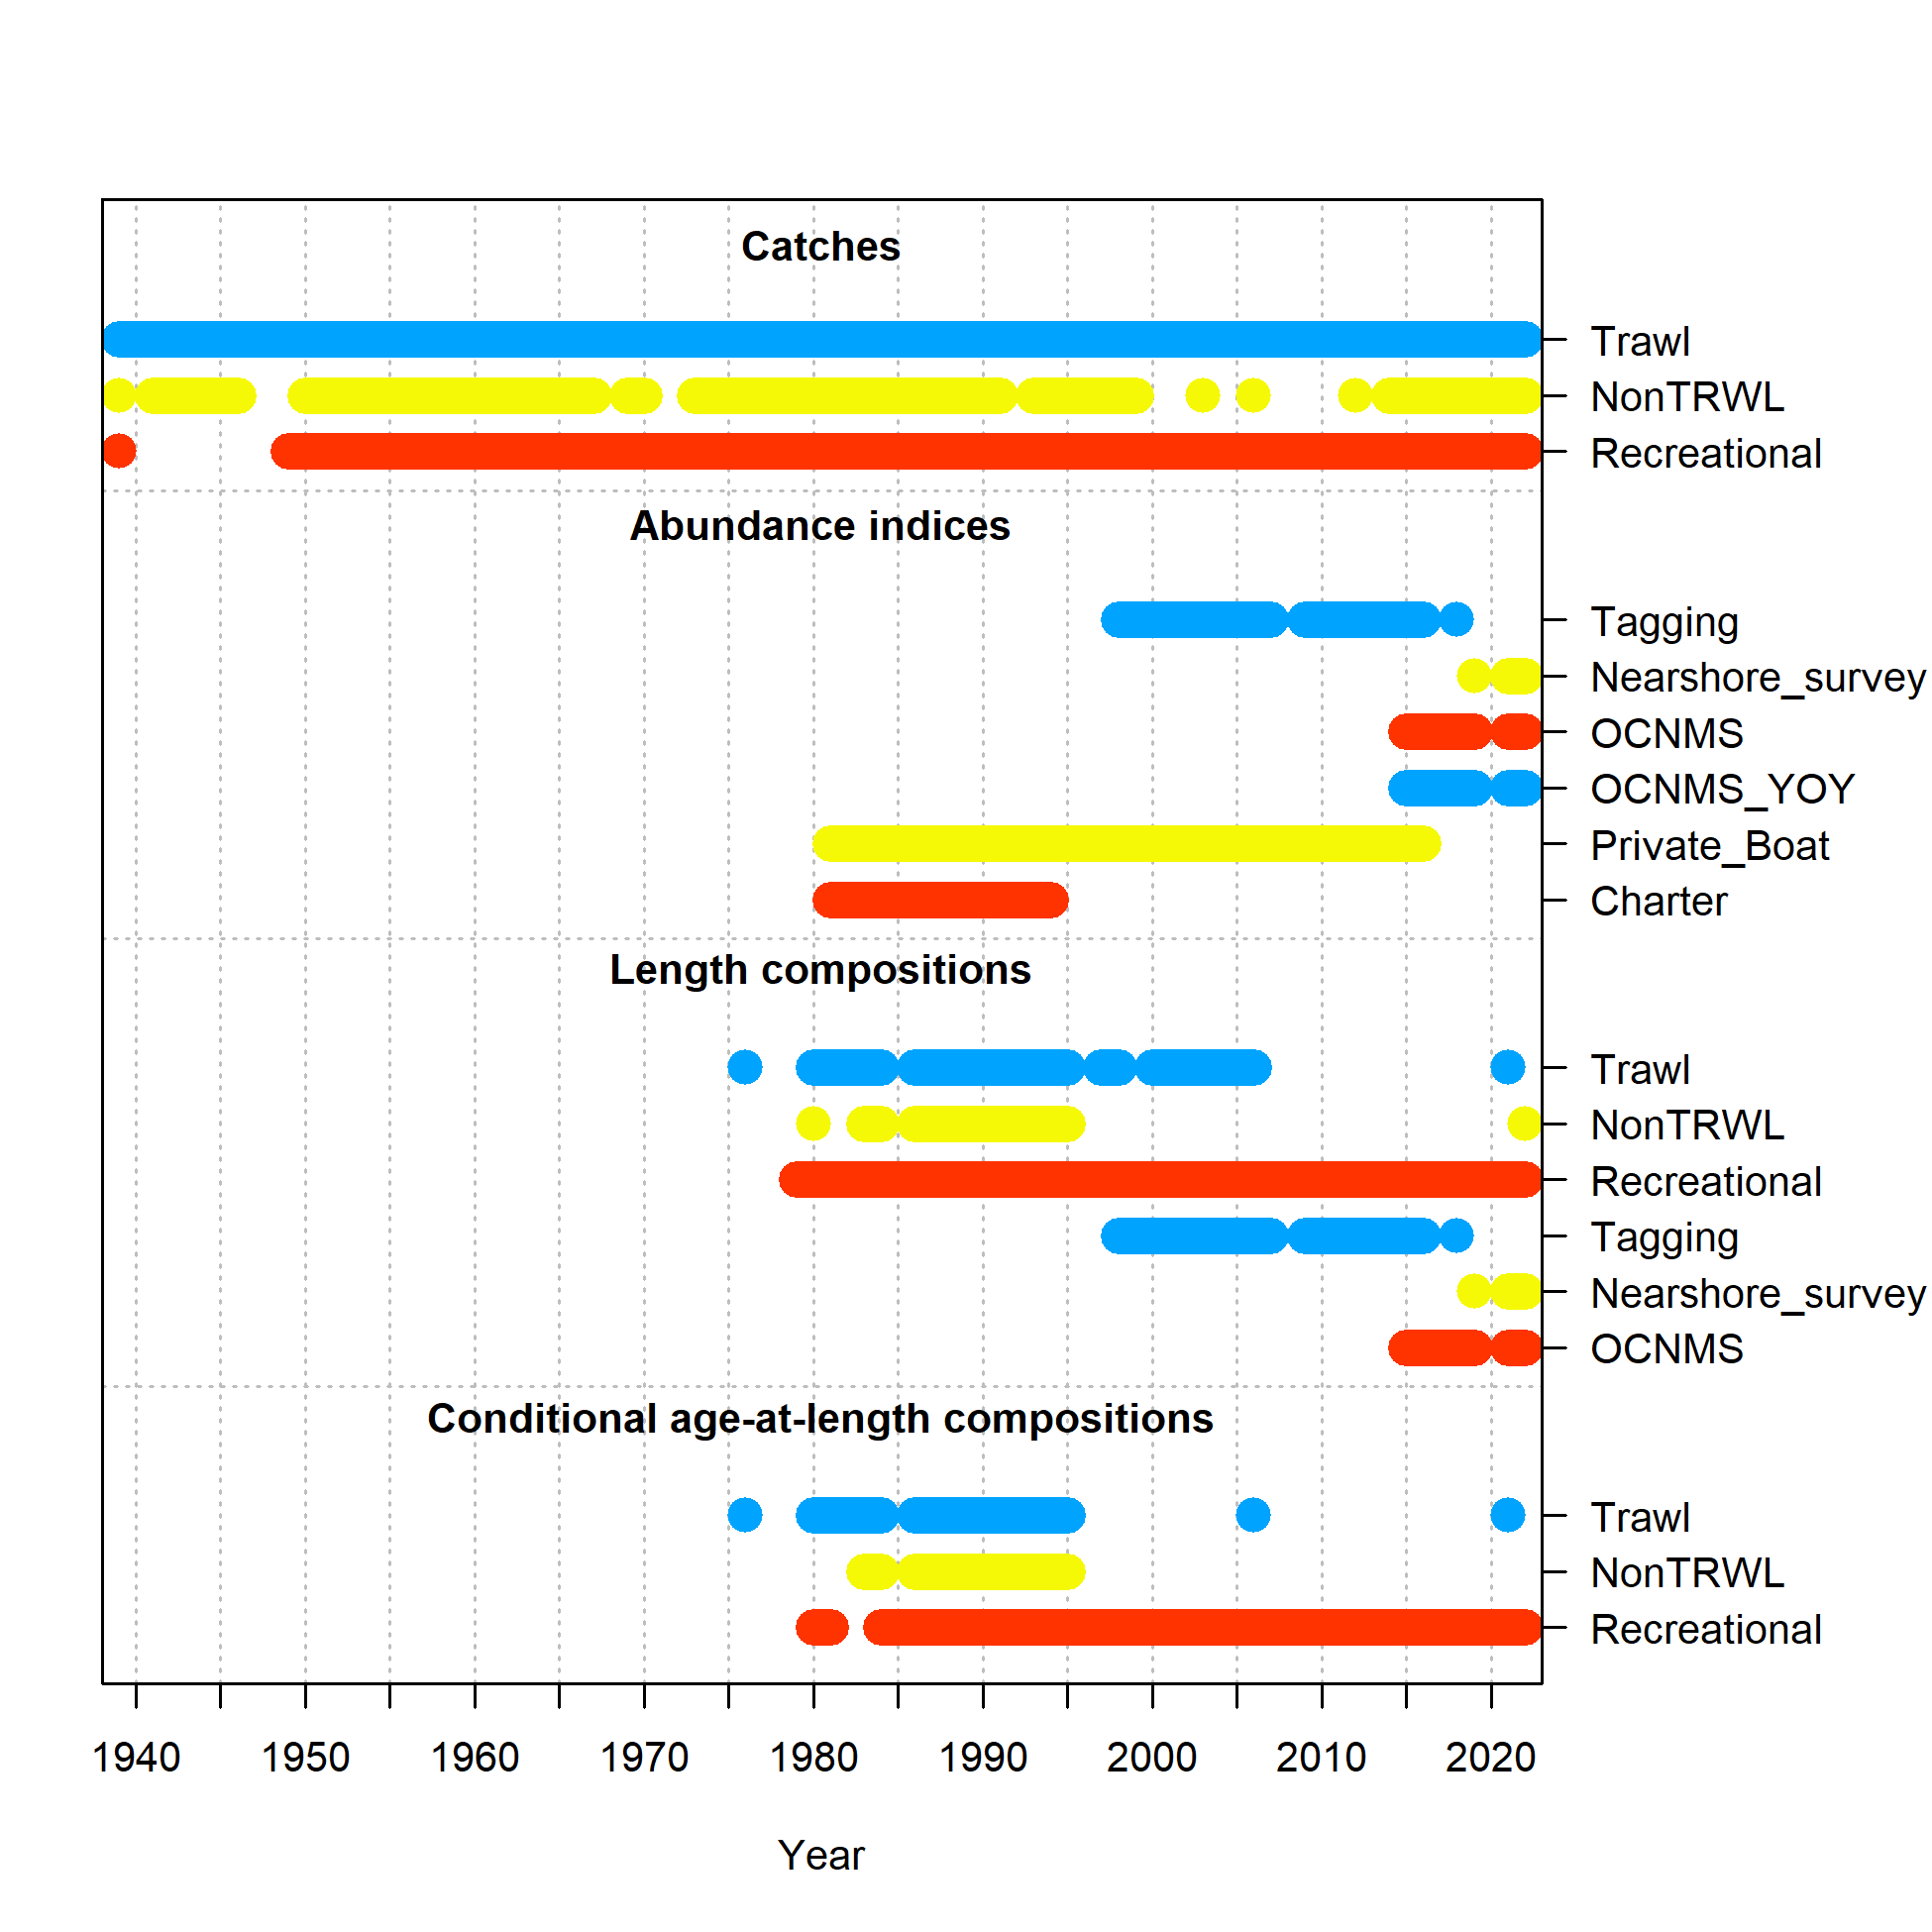
\includegraphics[width=1\textwidth,height=1\textheight]{C:/Users/Jason.Cope/Documents/Github/Sebastes_melanops_WA/Document/models/Reference model/plots/data_plot.png}
\caption{Summary of data sources used in the reference model.\label{fig:data-plot}}
\end{figure}
\end{document}
